%**************************************************************************************
% License:
% CC BY-NC-SA 4.0 (http://creativecommons.org/licenses/by-nc-sa/4.0/)
%**************************************************************************************

\documentclass[notes]{beamer}

\mode<presentation> {

\usetheme{Madrid}

% Burnt orange
\definecolor{burntorange}{rgb}{0.8, 0.33, 0.0}
\colorlet{beamer@blendedblue}{burntorange}
% Pale yellow
\definecolor{paleyellow}{rgb}{1.0, 1.0, 0.953}
\setbeamercolor{background canvas}{bg=paleyellow}
% Secondary and tertiary palett
\setbeamercolor*{palette secondary}{use=structure,fg=white,bg=burntorange!80!black}
\setbeamercolor*{palette tertiary}{use=structure,fg=white,bg=burntorange!60!black}

% To remove the footer line in all slides uncomment this line
%\setbeamertemplate{footline}
% To replace the footer line in all slides with a simple slide count uncomment this line
%\setbeamertemplate{footline}[page number]

% To remove the navigation symbols from the bottom of all slides uncomment this line
%\setbeamertemplate{navigation symbols}{}
}

\usepackage{amsmath}
\usepackage{bm}
\usepackage{breqn}
\usepackage{graphicx} % for figures
\usepackage{subcaption} % for subplots 
\usepackage[labelsep=space,tableposition=top]{caption}
\renewcommand{\figurename}{Fig.} 
\usepackage{cleveref}
\usepackage{caption,subcaption}% http://ctan.org/pkg/{caption,subcaption}
\usepackage{booktabs} % Allows the use of \toprule, \midrule and \bottomrule in tables
\usepackage{multirow}

% To print 2 slides on a page
%\usepackage{handoutWithNotes}
%\pgfpagesuselayout{2 on 1}[border shrink=2mm]
%----------------------------------------------------------------------------------------
%	TITLE PAGE
%----------------------------------------------------------------------------------------
% The short title appears at the bottom of every slide, the full title is only on the title page
\title[CE394M: solvers - errors]{CE394M: FEM solvers and errors} 
\author{Krishna Kumar} % name
\institute[UT Austin] % institution 
{
University of Texas at Austin \\
\medskip
\textit{
  \url{krishnak@utexas.edu}} % Your email address
}
\date{\today} % Date, can be changed to a custom date

\begin{document}

\begin{frame}
\titlepage % title page as the first slide
\end{frame}

\begin{frame}
 % Table of contents slide, comment this block out to remove it
 \frametitle{Overview}
 % Throughout your presentation, if you choose to use \section{} and \subsection{} 
 % commands, these %will automatically be printed on this slide as an overview 
 \tableofcontents
\end{frame}

%----------------------------------------------------------------------------------------
% slides
%----------------------------------------------------------------------------------------
\section{Solving non-linear problems}
%------------------------------------------------
\begin{frame}
\frametitle{Linear and non-linear problems}
\begin{itemize}
	\item \textbf{Linear problems}
	\mode<beamer>{
		\begin{itemize}
			\item The response can only be approximated as linear if its
			deformations/motions are small.
			\item In linear analyses, the response to individual load cases can be
			scaled and added to the results from other linear analyses,
			which is the principle of superposition.
		\end{itemize}
	}
	\mode<handout>{
		\vspace{2.5cm}
	}
	%
	\item \textbf{Non-linear problems}
		\mode<beamer>{
		\begin{itemize}
			\item Superposition is invalid.
			\item The solution is an incremental/iterative process.
			\item An iteration is the solution of a system of equations linearised
			about the current state of the nonlinear physical problem.
		\end{itemize}
	}
	\mode<handout>{
		\vspace{2.5cm}
	}
	\end{itemize}
\end{frame}

%------------------------------------------------
\begin{frame}
\frametitle{Non-linearity in geotechnical engineering}
\mode<beamer>{
	\begin{itemize}
		\item \textbf{Material non-linearity}
			\begin{itemize}
				\item plasticity
			\end{itemize}

		\item \textbf{Contact}
			\begin{itemize}
				\item discontinuous source of non-linearity
			\end{itemize}
		
		\item \textbf{Large deformations and motions of a geotechnical structures}
			\begin{itemize}
				\item rotation, rigid body motion
				\item often ignored, still in the research area.
			\end{itemize}
	\end{itemize}
}
\mode<handout>{
	\vspace{3cm}
}
	%
\begin{figure}[ht]
	\centering
	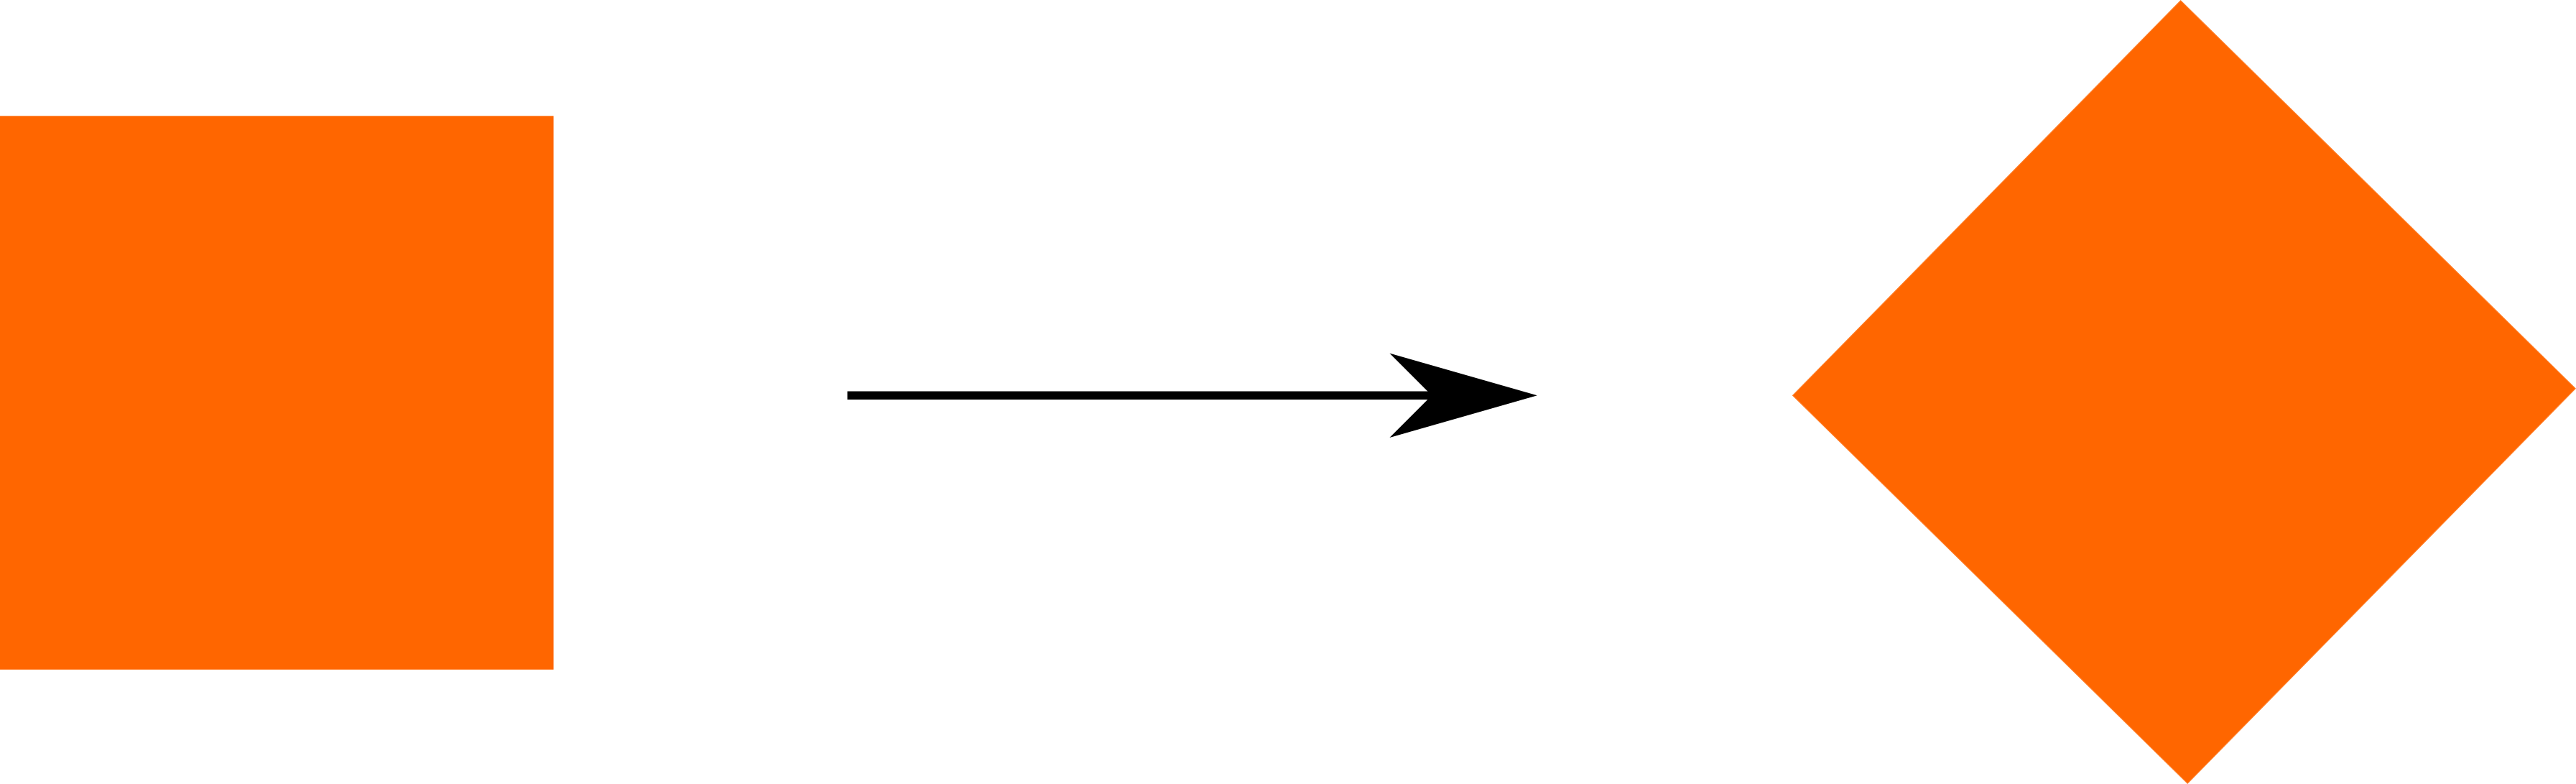
\includegraphics[width=0.85\textwidth]{figs/rotation.png}
	\caption*{No strains if linear strain-displacement relations are used.}
\end{figure}
\end{frame}

%------------------------------------------------
\begin{frame}
\frametitle{Linear solvers}
To solve a system of linear equations of the form $\mathbf{Ka = b}$, there are two families of
methods of solvers that can be used: direct and iterative.
\mode<beamer>{
	\begin{itemize}
		\item Direct solvers solve a system of linear equations in a predefined number of steps. 
		\item Methods are based on Gauss elimination, with the most common method being LU decomposition. 
		\item The time required to solve a linear system increases with the number of computer
		operations performed.
		\item For a direct linear solver applied to a dense system of size $n \times n$: CPU time = $C n^3$.
		\item If the number of degrees of freedom in a finite element simulation is doubled,
		the time required to solve the system will increase by a factor of 8!
	\end{itemize}
}
\mode<handout>{
	\vspace{6cm}
}
\end{frame}
\subsection{Iterative solvers}
%------------------------------------------------
\begin{frame}
\frametitle{Iterative solvers}
The system of equations that we derived from the finite element approximation of the BVP:
\mode<beamer>{
		\begin{equation*}
			F_{\mathrm{int}}(u) - F_{\mathrm{ext}} = 0
		\end{equation*}

At this point we remind ourselves that in the case of finite deformations, both $F_{\mathrm{int}}$ and $F_{\mathrm{ext}}$ are in general very nonlinear terms. 

The integration has to be carried over the current volume and surface (of the finite element under consideration) that may in general depend on $u$ in a highly non-linear fashion.
}
\mode<handout>{
	\vspace{6cm}
}
\end{frame}

\subsection{Tangent stiffness}
%------------------------------------------------
\begin{frame}
\frametitle{Tangent stiffness method}
\mode<beamer>{
	\begin{figure}[ht]
		\centering
		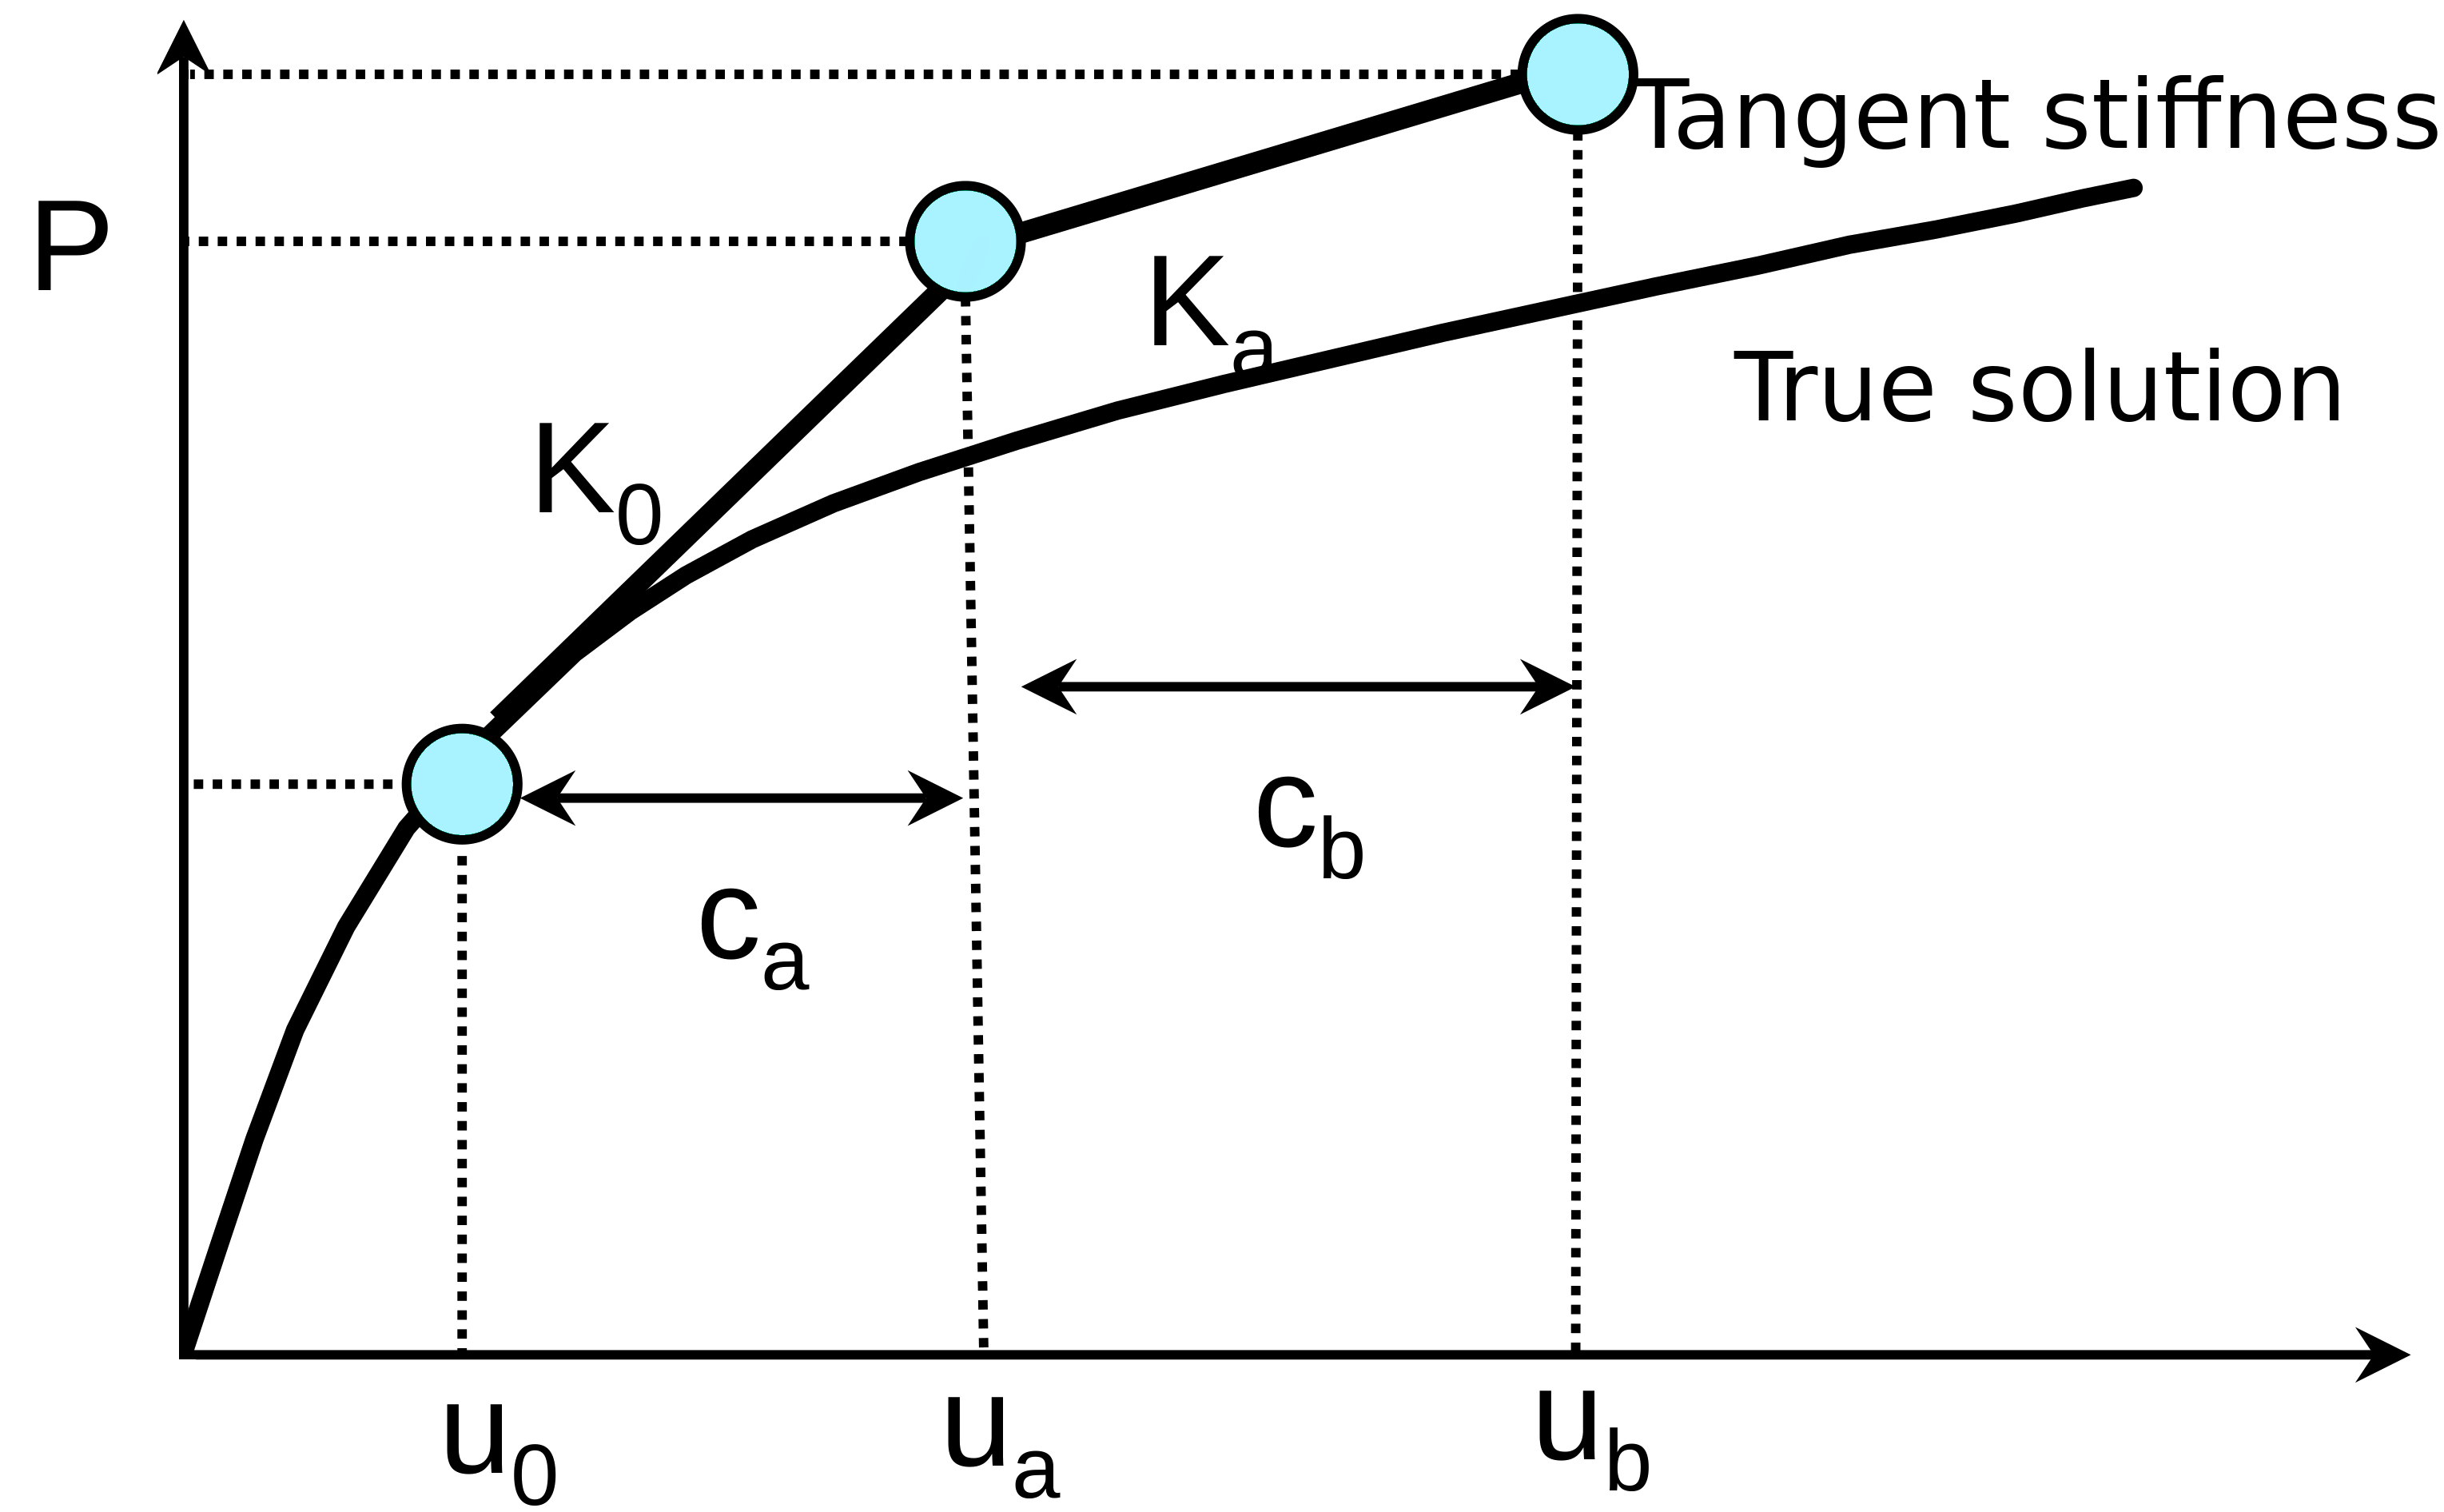
\includegraphics[width=0.65\textwidth]{figs/tangent-stiffness.png}
	\end{figure}
	\begin{itemize}
		\item Many small increments are need to obtain accurate solution
		\item Need to perform a parametric study to find the optimum incremental
		\item Defining increments is very important
		\item Program - SAGE CRISP
	\end{itemize}
}
\mode<handout>{
	\vspace{6cm}
}
\end{frame}

\note {
	\begin{figure}[ht]
		\centering
		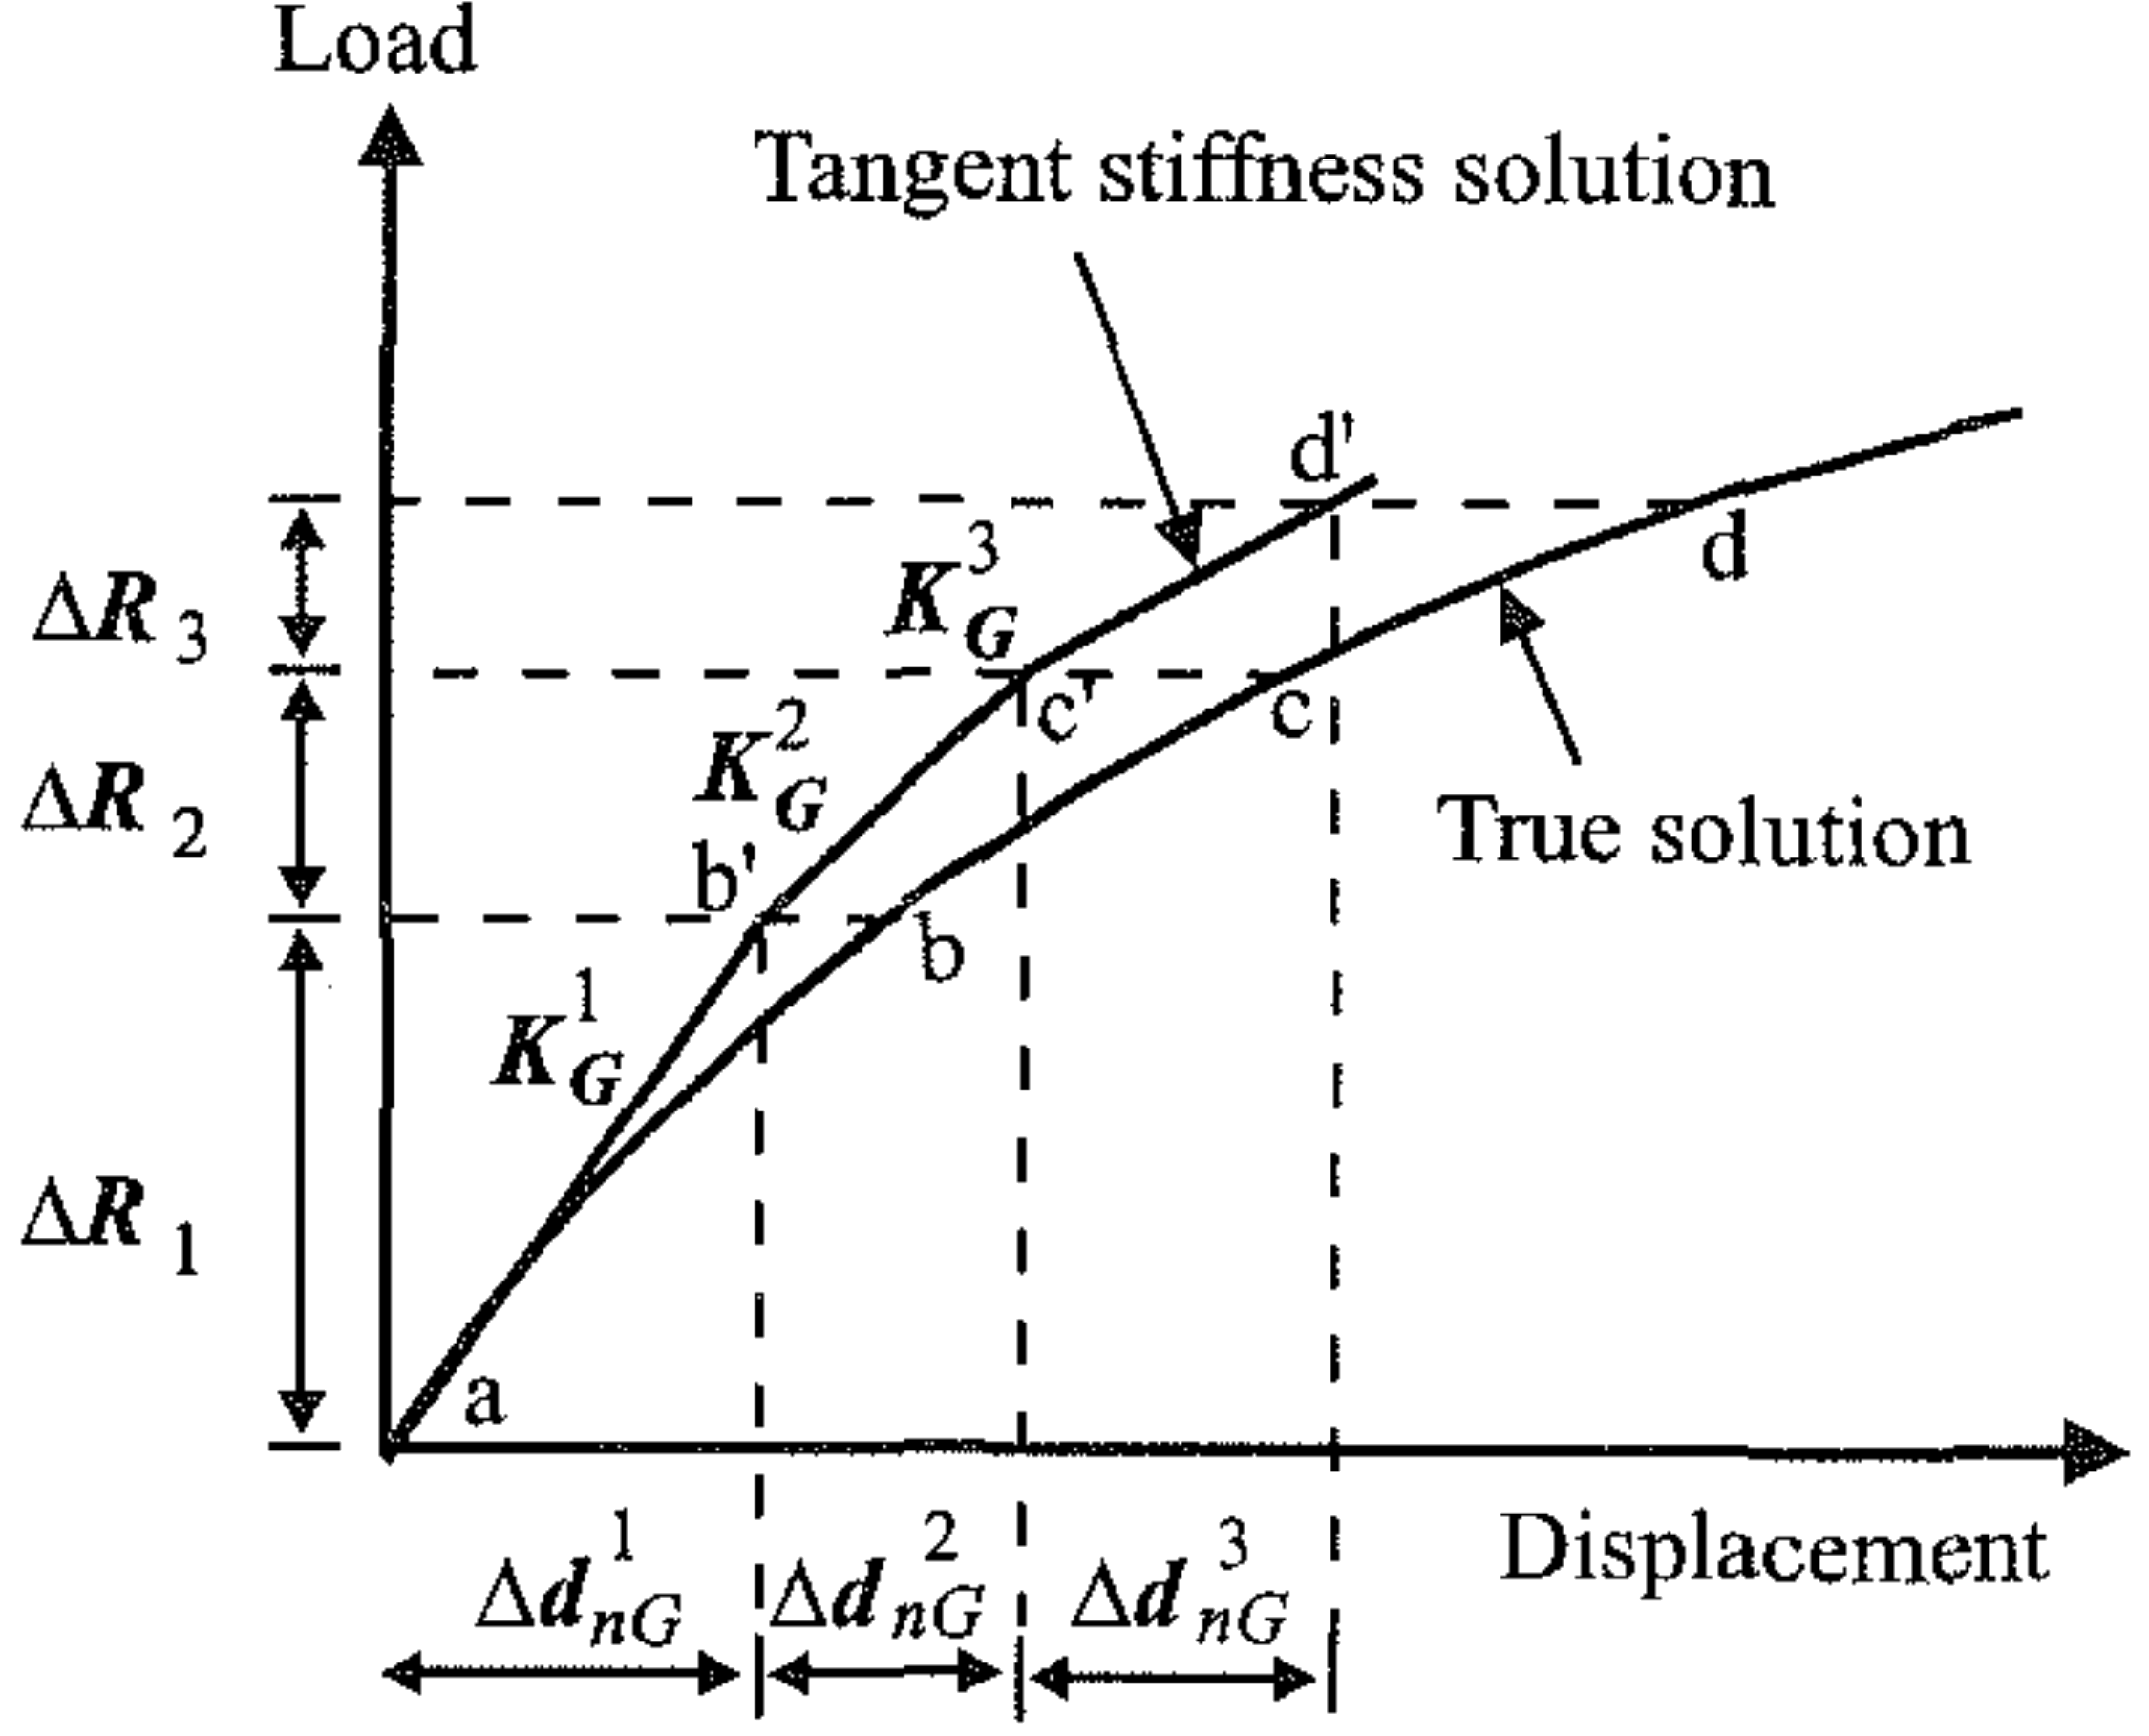
\includegraphics[width=0.65\textwidth]{figs/tangent-stiffness-explained.png}
	\end{figure}	
}
\note {
The analysis starts with the application of $\Delta R$. The incremental global stiffness matrix $\left[\mathbf{K}_G\right]^1$ for this increment is evaluated based on the unstressed state of the bar
corresponding to point `\textit{a}'. For an elasto-plastic material this might be constructed
using the elastic constitutive matrix $[\mathbf{D}]$. Equation is then solved to determine the nodal displacements ${\Delta d}^1$. As the material stiffness is assumed to remain constant, the load displacement curve follows the straight line $ab^\prime$. In reality, the stiffness of the material does not remain constant during this loading
increment and the true solution is represented by the curved path `\textit{ab}'. There is therefore an error in the predicted displacement equal to the distance `$b^\prime b$', however in the tangent stiffness
Load approach this error is neglected. The
second increment of load, $\Delta R^2$, is then
applied, with the incremental global 
stiffness matrix $\left[\mathbf{K}_G\right]^2$ evaluated using the stresses and strains appropriate to
the end of increment 1, i.e. point 'b.'
}
\note{
	In the incremental solution we divide the load into increments $\Delta P = \lambda P$, where $\lambda$ is also known as a load factor and apply a repeated solution of $\Delta u = K^{-1} \Delta P$. \\
	
	Basically we divide the load into substeps, and treat each as linear - but that is usually not accurate enough and inefficient.
}
\subsection{Newton Raphson}
%------------------------------------------------
\begin{frame}
\frametitle{Newton Raphson method}
\mode<beamer>{
	\begin{figure}[ht]
		\centering
		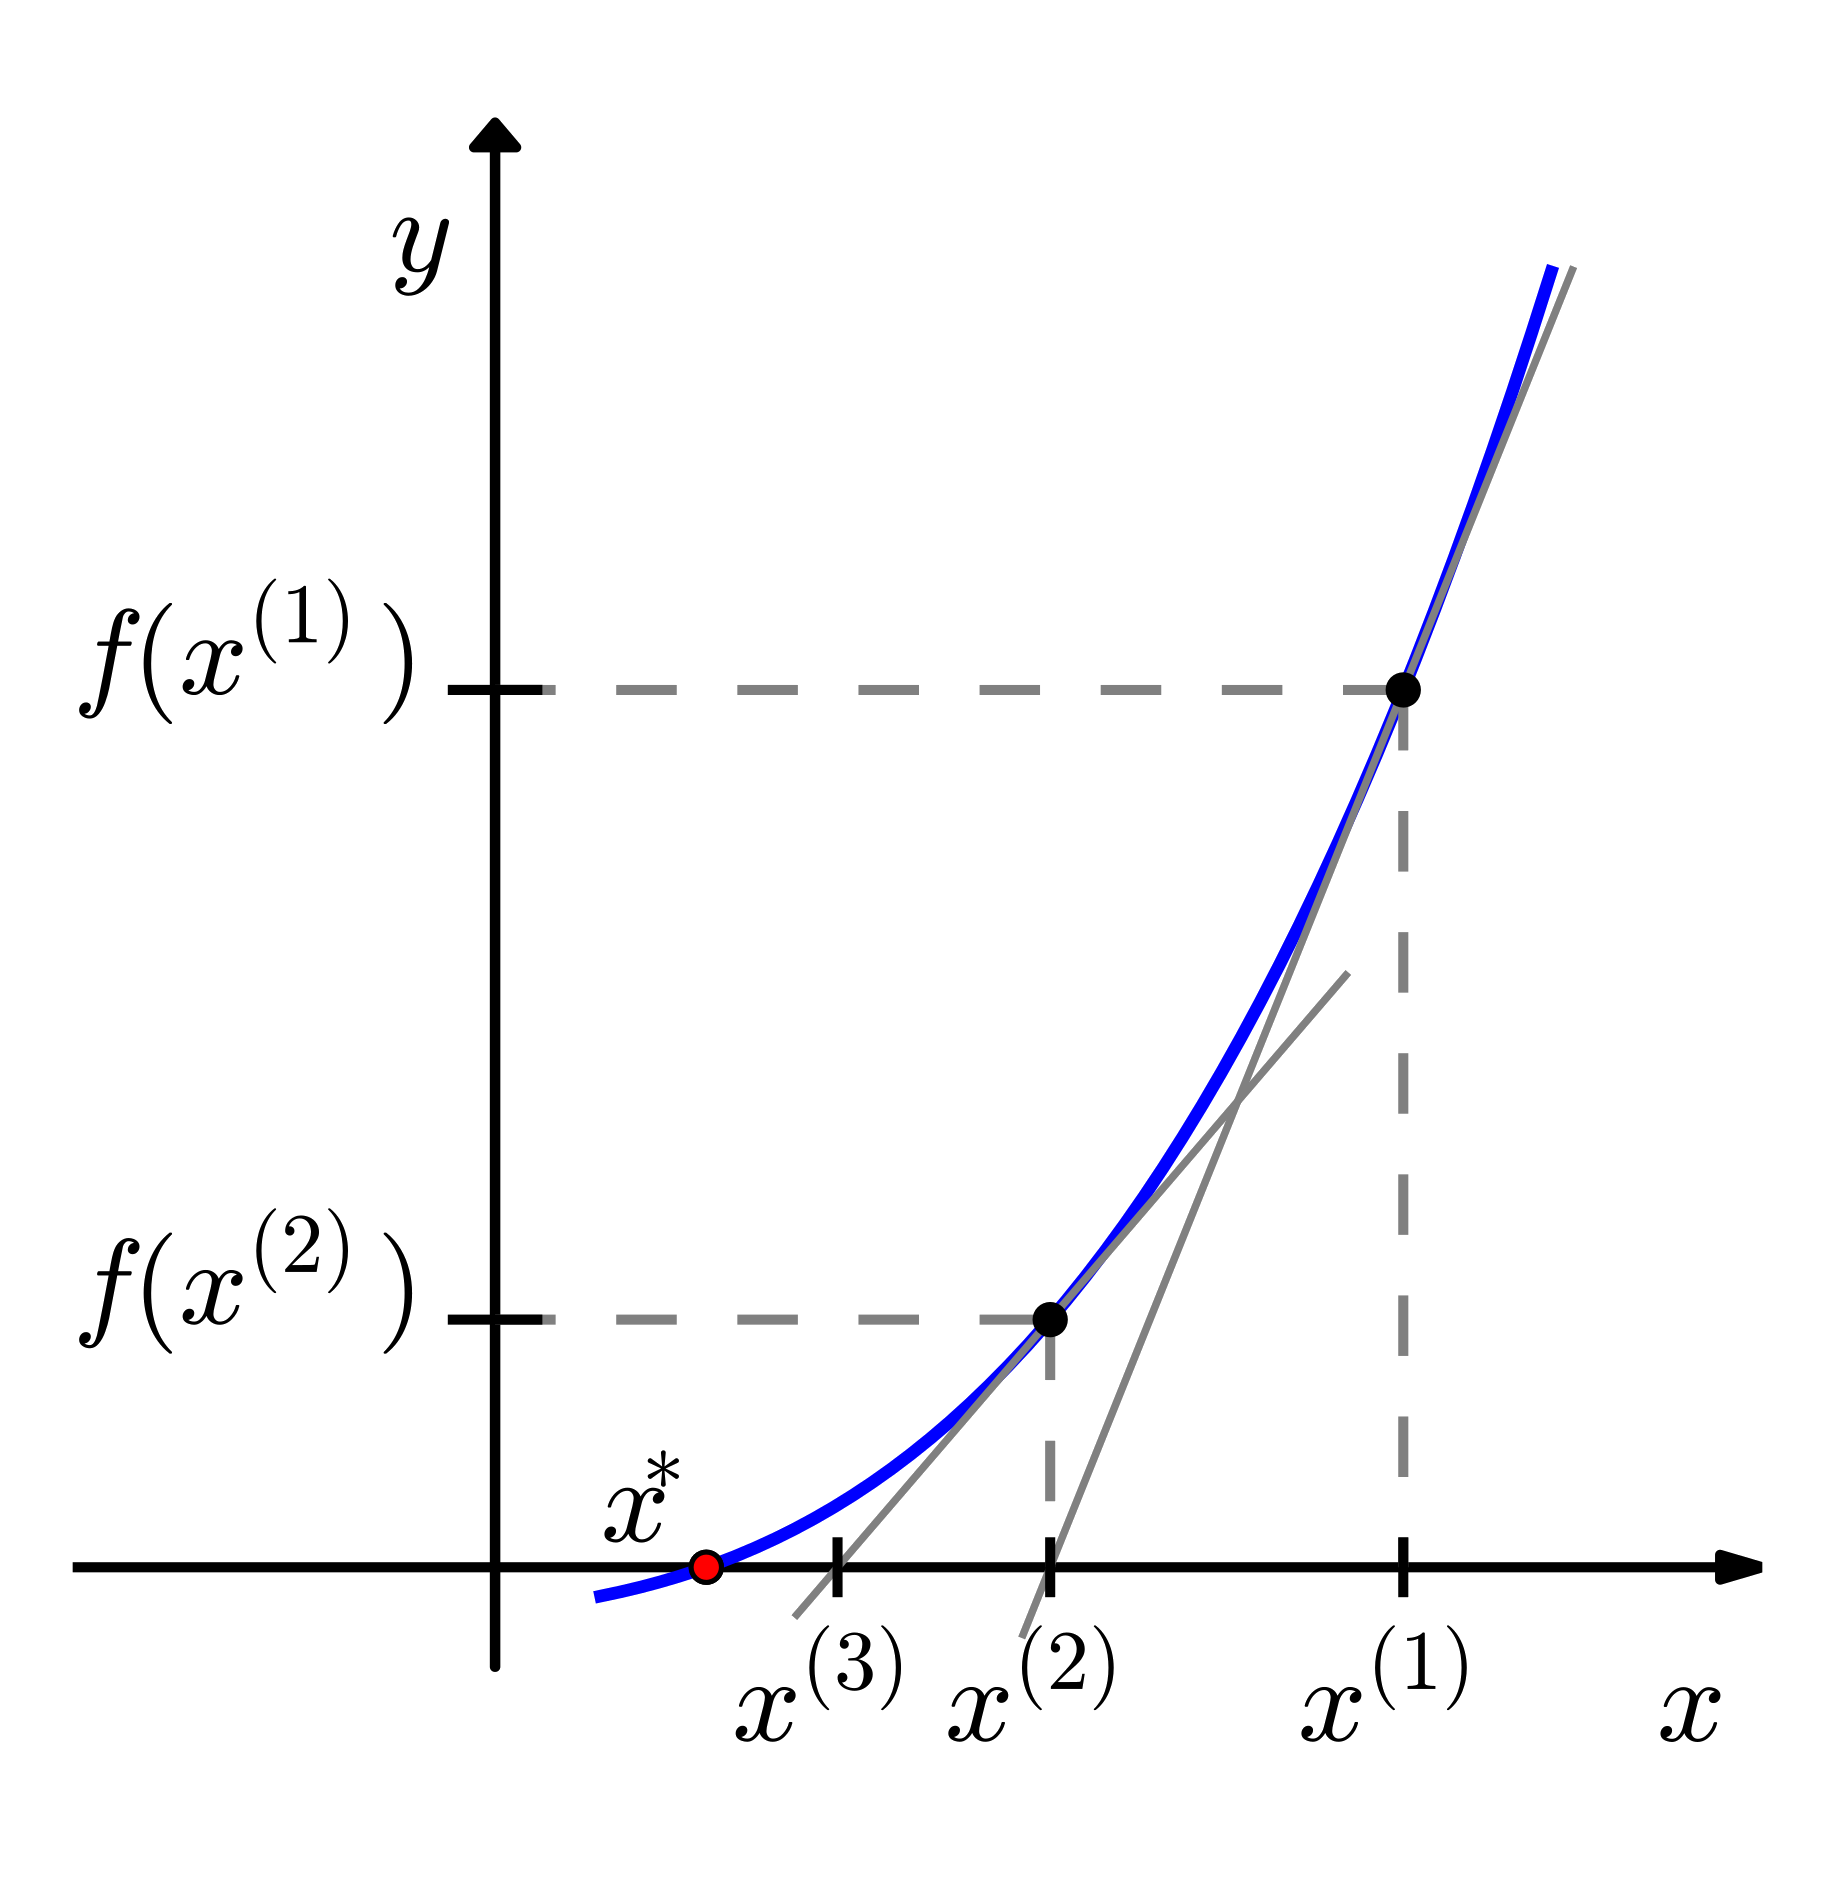
\includegraphics[width=0.5\textwidth]{figs/newton.png}
	\end{figure}
	\begin{equation*}
		x_{n+1} = x_n - \frac{f(x_n)}{f^\prime(x_n)}
	\end{equation*}
}
\mode<handout>{
	\vspace{6cm}
}
\end{frame}

%------------------------------------------------
\begin{frame}
\frametitle{Newton Raphson method}
The incremental loading is expressed as follows. The external load vector $F_{\mathrm{ext}}$ is gradually increased from 0 in order to reach a desired value $\mathbf{F}^*$. Assuming that  $\mathbf{F}^*$ itself remains constant during the analysis in terms of its 'direction' and only its magnitude is changing, we can write $F_{\mathrm{ext}} = q$ known just to simplify our expression for the system of equations. Then we can control how the external load vector increases or decreases by introducing a scalar quantity $\lambda$ and express the system as follows:

\mode<beamer>{
	\begin{equation*}
		R(u) = F_{\mathrm{int}} - F_{\mathrm{ext}} \rightarrow R(u) = F_{\mathrm{int}} - \lambda F_{\mathrm{ext}} = 0
	\end{equation*}
}
\mode<handout>{
\vspace{6cm}
}
	
Thus by increasing or decreasing $\lambda$ we can control our load. We are interested in 
$u$ and $\lambda$. At every increment, we change slightly the value of $\lambda$ and try 
to determine $u$ satisfying $R(u)= 0$.
	
\mode<beamer>{
	\begin{equation*}
		\Delta u = [K_T]^{-1}_{u0} \cdot (\Delta \lambda q)
	\end{equation*}
}
\mode<handout>{
\vspace{6cm}
}
	
\end{frame}

\note {
	where $\left[K^T\right] = [\partial F(u)/ \partial u]$ is the ``Jacobian'' matrix of the system of equations and is commonly referred to as the Stiffness Matrix.
	\begin{figure}[ht]
		\centering
		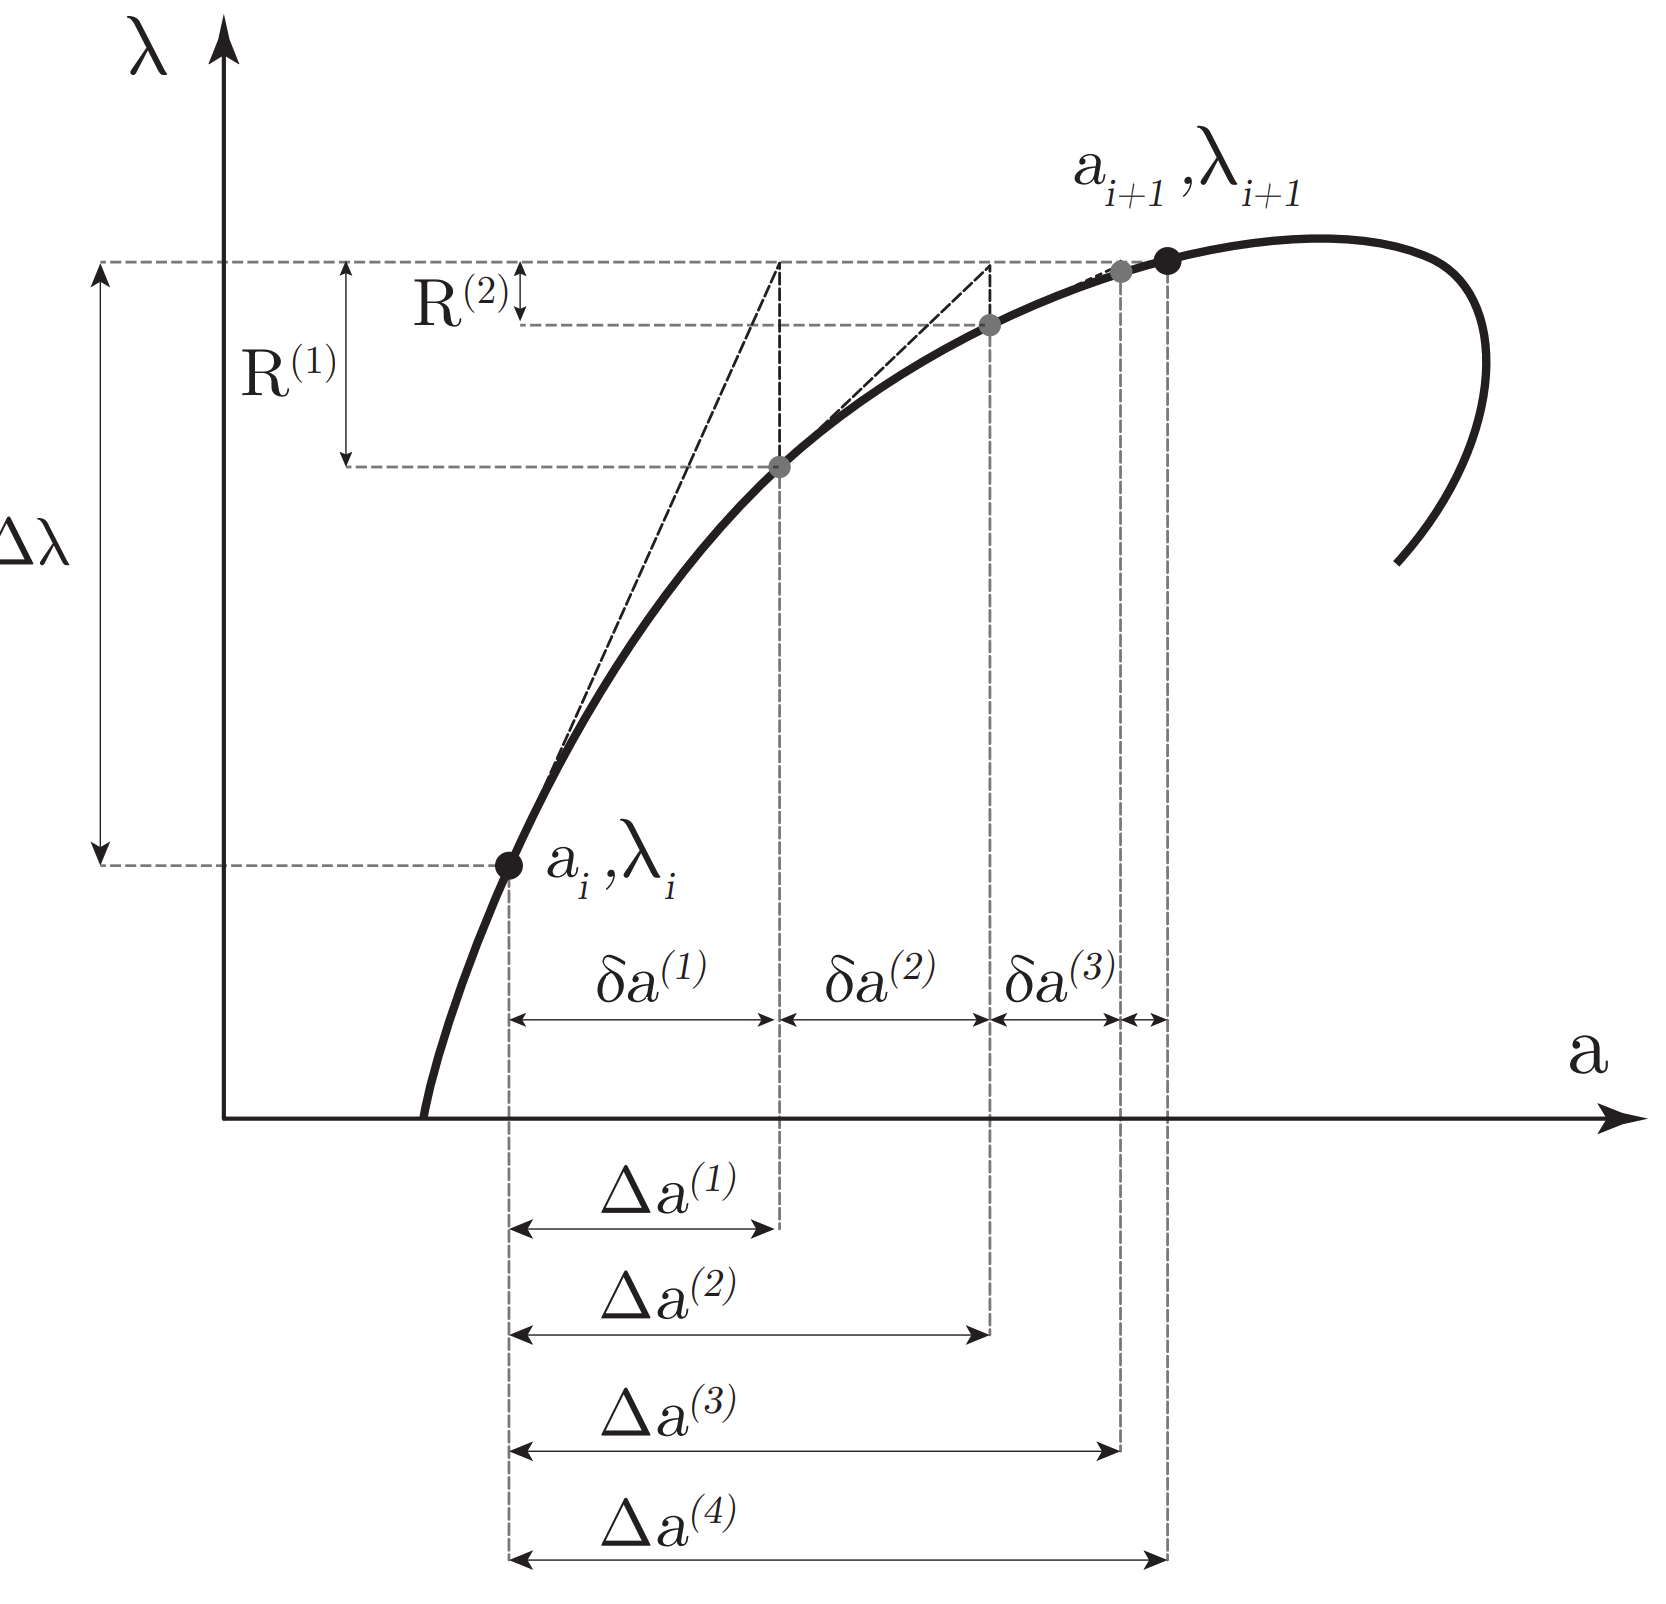
\includegraphics[width=0.65\textwidth]{figs/newton-raphson-fe.png}
	\end{figure}
}

%------------------------------------------------
\begin{frame}
\frametitle{Newton Raphson method}
\mode<beamer>{
	\begin{figure}[ht]
		\centering
		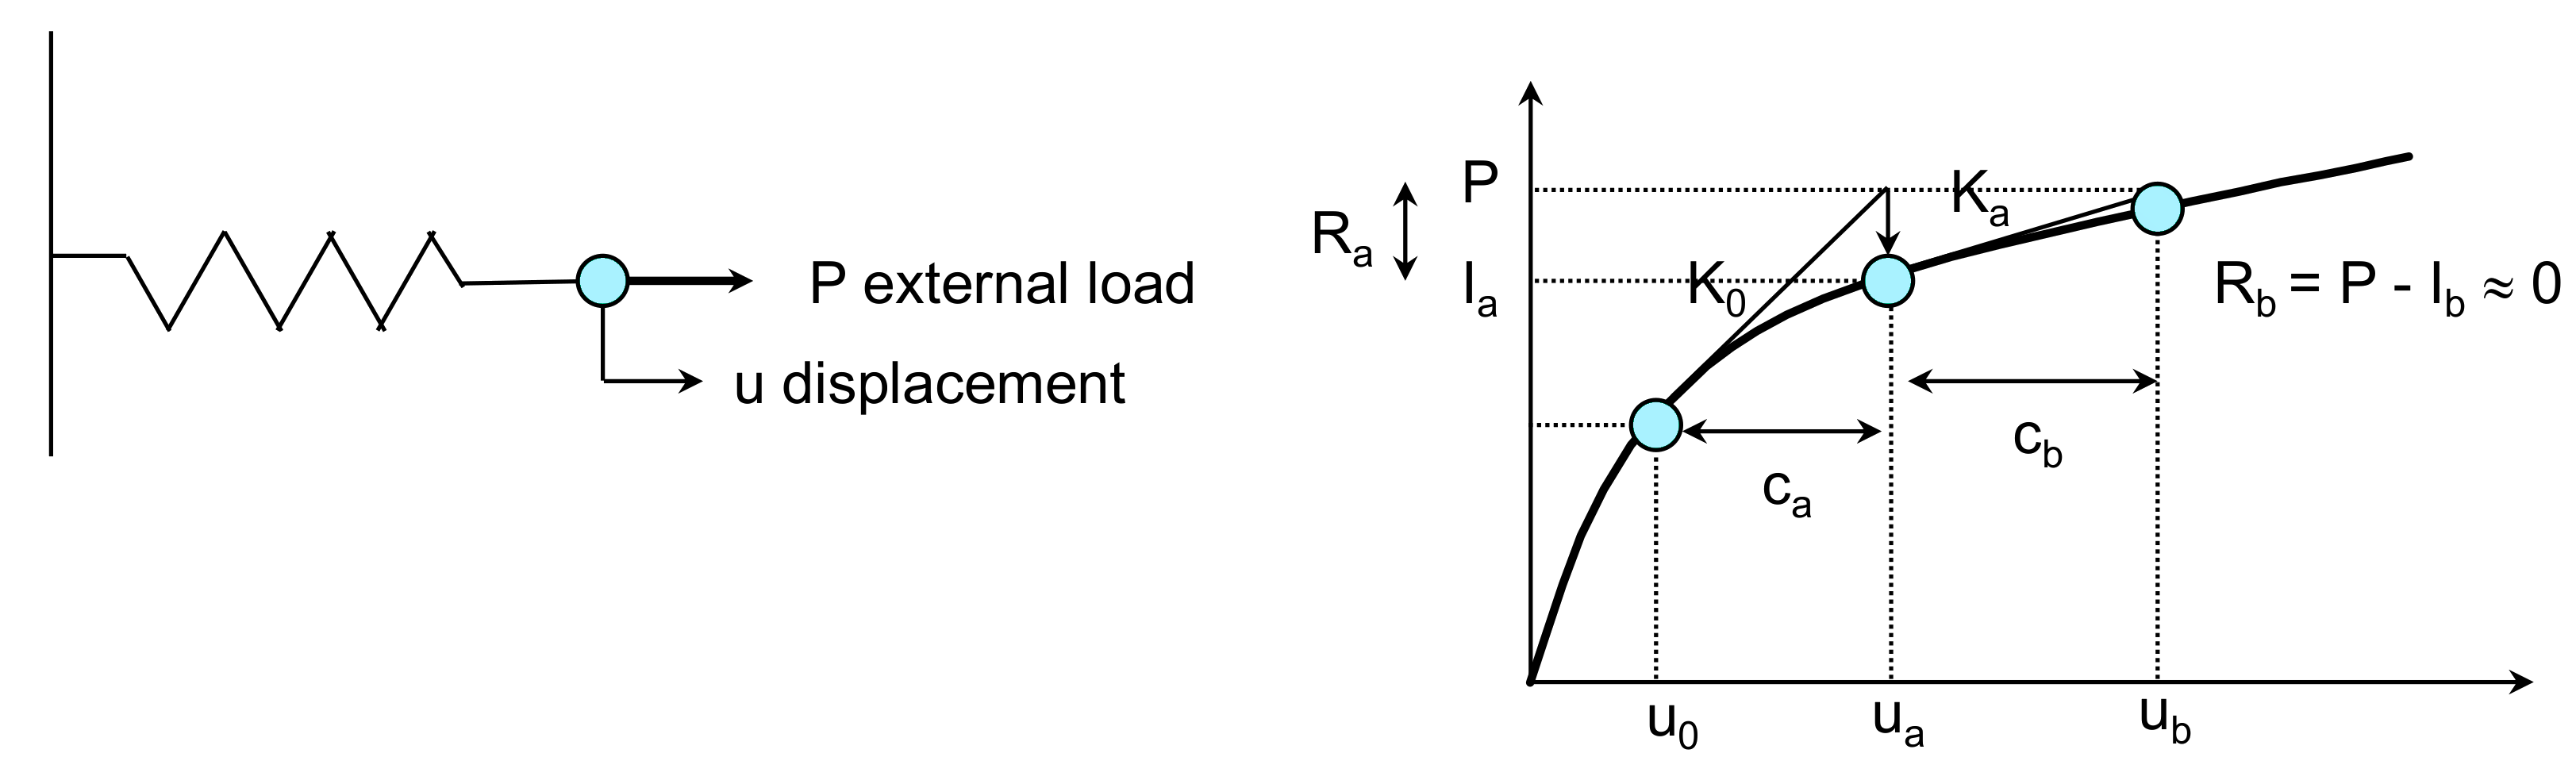
\includegraphics[width=\textwidth]{figs/newton-raphson.png}
	\end{figure}
	\begin{itemize}
		\item Using the initial stiffness $K_0$, apply an increment of load $\delta P$,
		calculate an approximate solution $c_a$ caused by this increment.
		
		\item The stiffness $K_a$ is updated using the new position, and the
		internal force in the spring $I_a$ is calculated.
		
		\item If the difference $R_a$ between the total load applied to the spring,
		$P$, and $I_a$ is smaller than the tolerance, $u_a = u_0 + c_a$ is the
		converged solution.
	\end{itemize}
}
\mode<handout>{
	\vspace{6cm}
}
\end{frame}

\note{
	\begin{itemize}
		\item If $R_a$ is not small, a new displacement correction $c_b$ is calculated
		by solving $c_b = R_a /K_a$
		\item The new displacement $u_b$ is updated, and the internal force $I_b$ in
		the updated configuration is calculated.
		\item The new force residual $R_b$ is obtained. If $R_b < tolerance$, the
		solution is converged. If not, continue the iteration.
	\end{itemize}
}


%------------------------------------------------
\begin{frame}
\frametitle{Newton Raphson method: Tolerance and Convergence}
\begin{itemize}
	\item Program - ABAQUS
	\item Newton-Raphson is the most standard method to solve nonlinear problems in FE.
	\item A large error in the initial estimate can contribute to non-convergence of the algorithm.
	\item \textbf{Tolerance}
	\begin{itemize}
		\item must be small enough to ensure that the approximate
		solution is close to the exact mathematical solution.
		\item must be large enough so that reasonable number of
		iterations are performed.
	\end{itemize}
	\item \textbf{Quadratic convergence}
	\begin{itemize}
		\item If the tangent stiffness is calculated correctly, $R$ should
		reduce quadratically from one iteration to the next.
	\end{itemize}
\end{itemize}
\end{frame}

%------------------------------------------------
\begin{frame}
\frametitle{Tangent-Stiffness vs Newton Raphson}
\begin{figure}[ht]
	\centering
	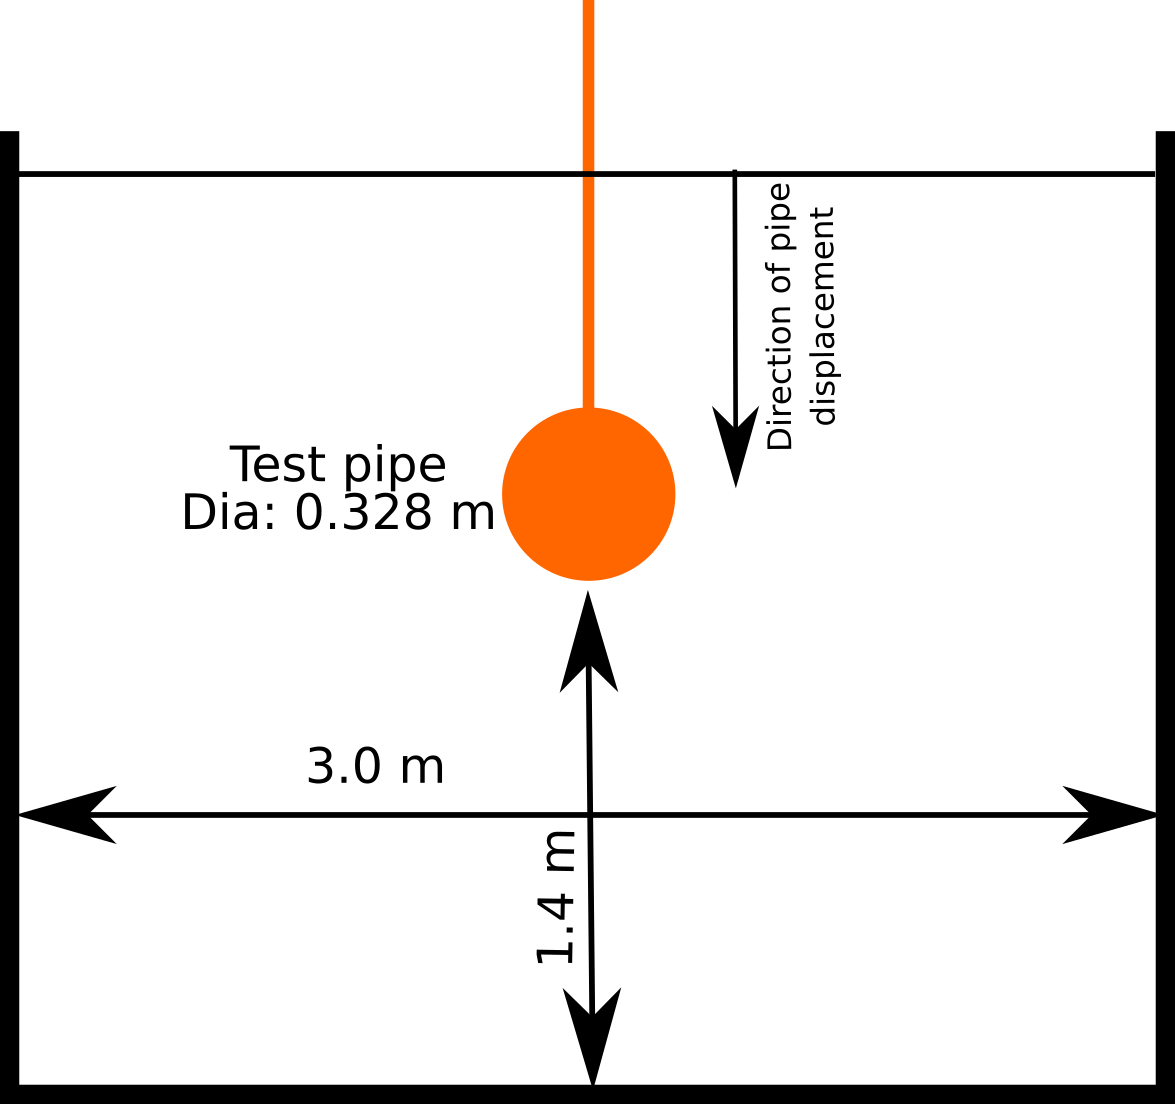
\includegraphics[width=0.65\textwidth]{figs/pipe-comparison-nr-tangent-stiffness.png}
\end{figure}
\end{frame}

%------------------------------------------------
\begin{frame}
\frametitle{Tangent-Stiffness vs Newton Raphson}
\begin{figure}[ht]
	\centering
	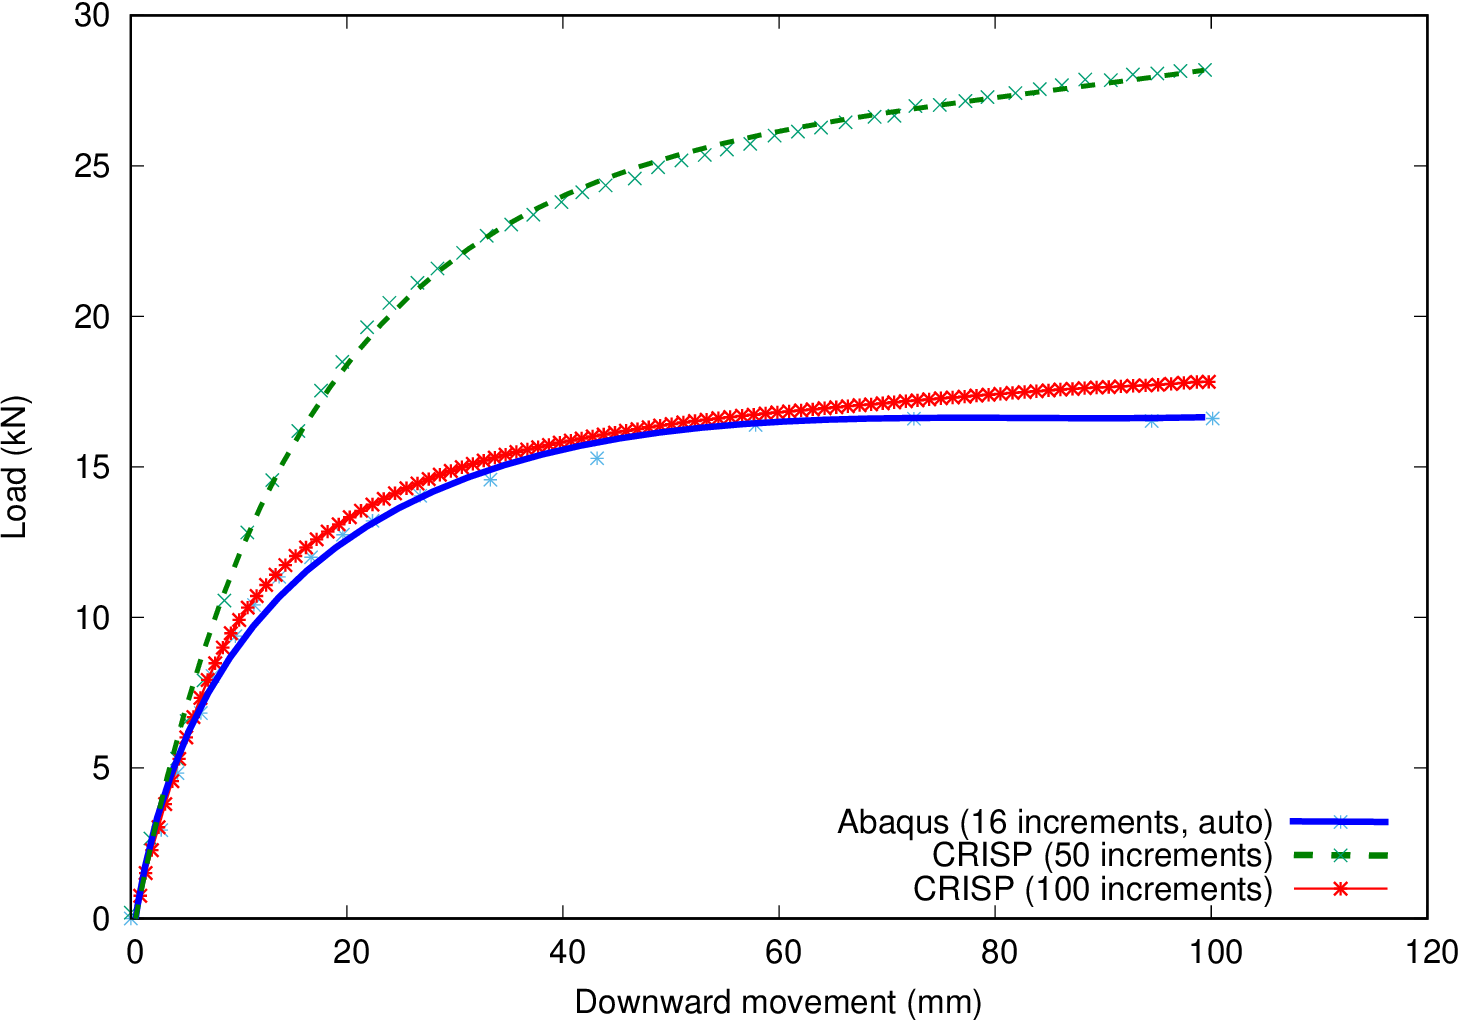
\includegraphics[width=0.85\textwidth]{figs/nr-tangent-stiffness.png}
\end{figure}
\end{frame}

%------------------------------------------------
\begin{frame}
\frametitle{Newton Raphson iterative procedure: FE example}
In Newton's method:
\mode<beamer>{
	\begin{equation*}
		{R} \equiv [K]{u} -{F} = 0
	\end{equation*}
}
\mode<handout>{
	\vspace{1.5cm}
}

where ${\mathbf{R}}$ is the residual vector, we expand ${\mathbf{R}}$ in Taylor's series:
	\begin{equation*}
		{\mathbf{R({u^{r+1}})}} = {\mathbf{R({u^{r}})}} + \left(\frac{\partial \mathbf{R}}{\partial\mathbf{u}}\right)^{(r)}\cdot {\delta \mathbf{u}} + \dots
	\end{equation*}
	Omitting higher order terms (2):
	\begin{align*}
		\left(\frac{\partial \mathbf{R}}{\partial\mathbf{u}}\right)^{(r)}\cdot {\delta \mathbf{u}} & = -{\mathbf{R({u^{r}})}} \\
		\left[\mathbf{T({u})^r}\right]{\delta \mathbf{u}} & = -{\mathbf{R({u^{r}})}} \\
	\end{align*}

where $[T]$ is called the \textit{tangent matrix}

\mode<beamer>{
	\begin{equation*}
	\left[\mathbf{T({u})^r}\right] \equiv \left(\frac{\partial \mathbf{R}}{\partial\mathbf{u}}\right)^{(r)}
	\end{equation*}
}
\end{frame}

%------------------------------------------------
\begin{frame}
\frametitle{Newton Raphson iterative procedure: FE example}
\begin{figure}[ht]
	\centering
	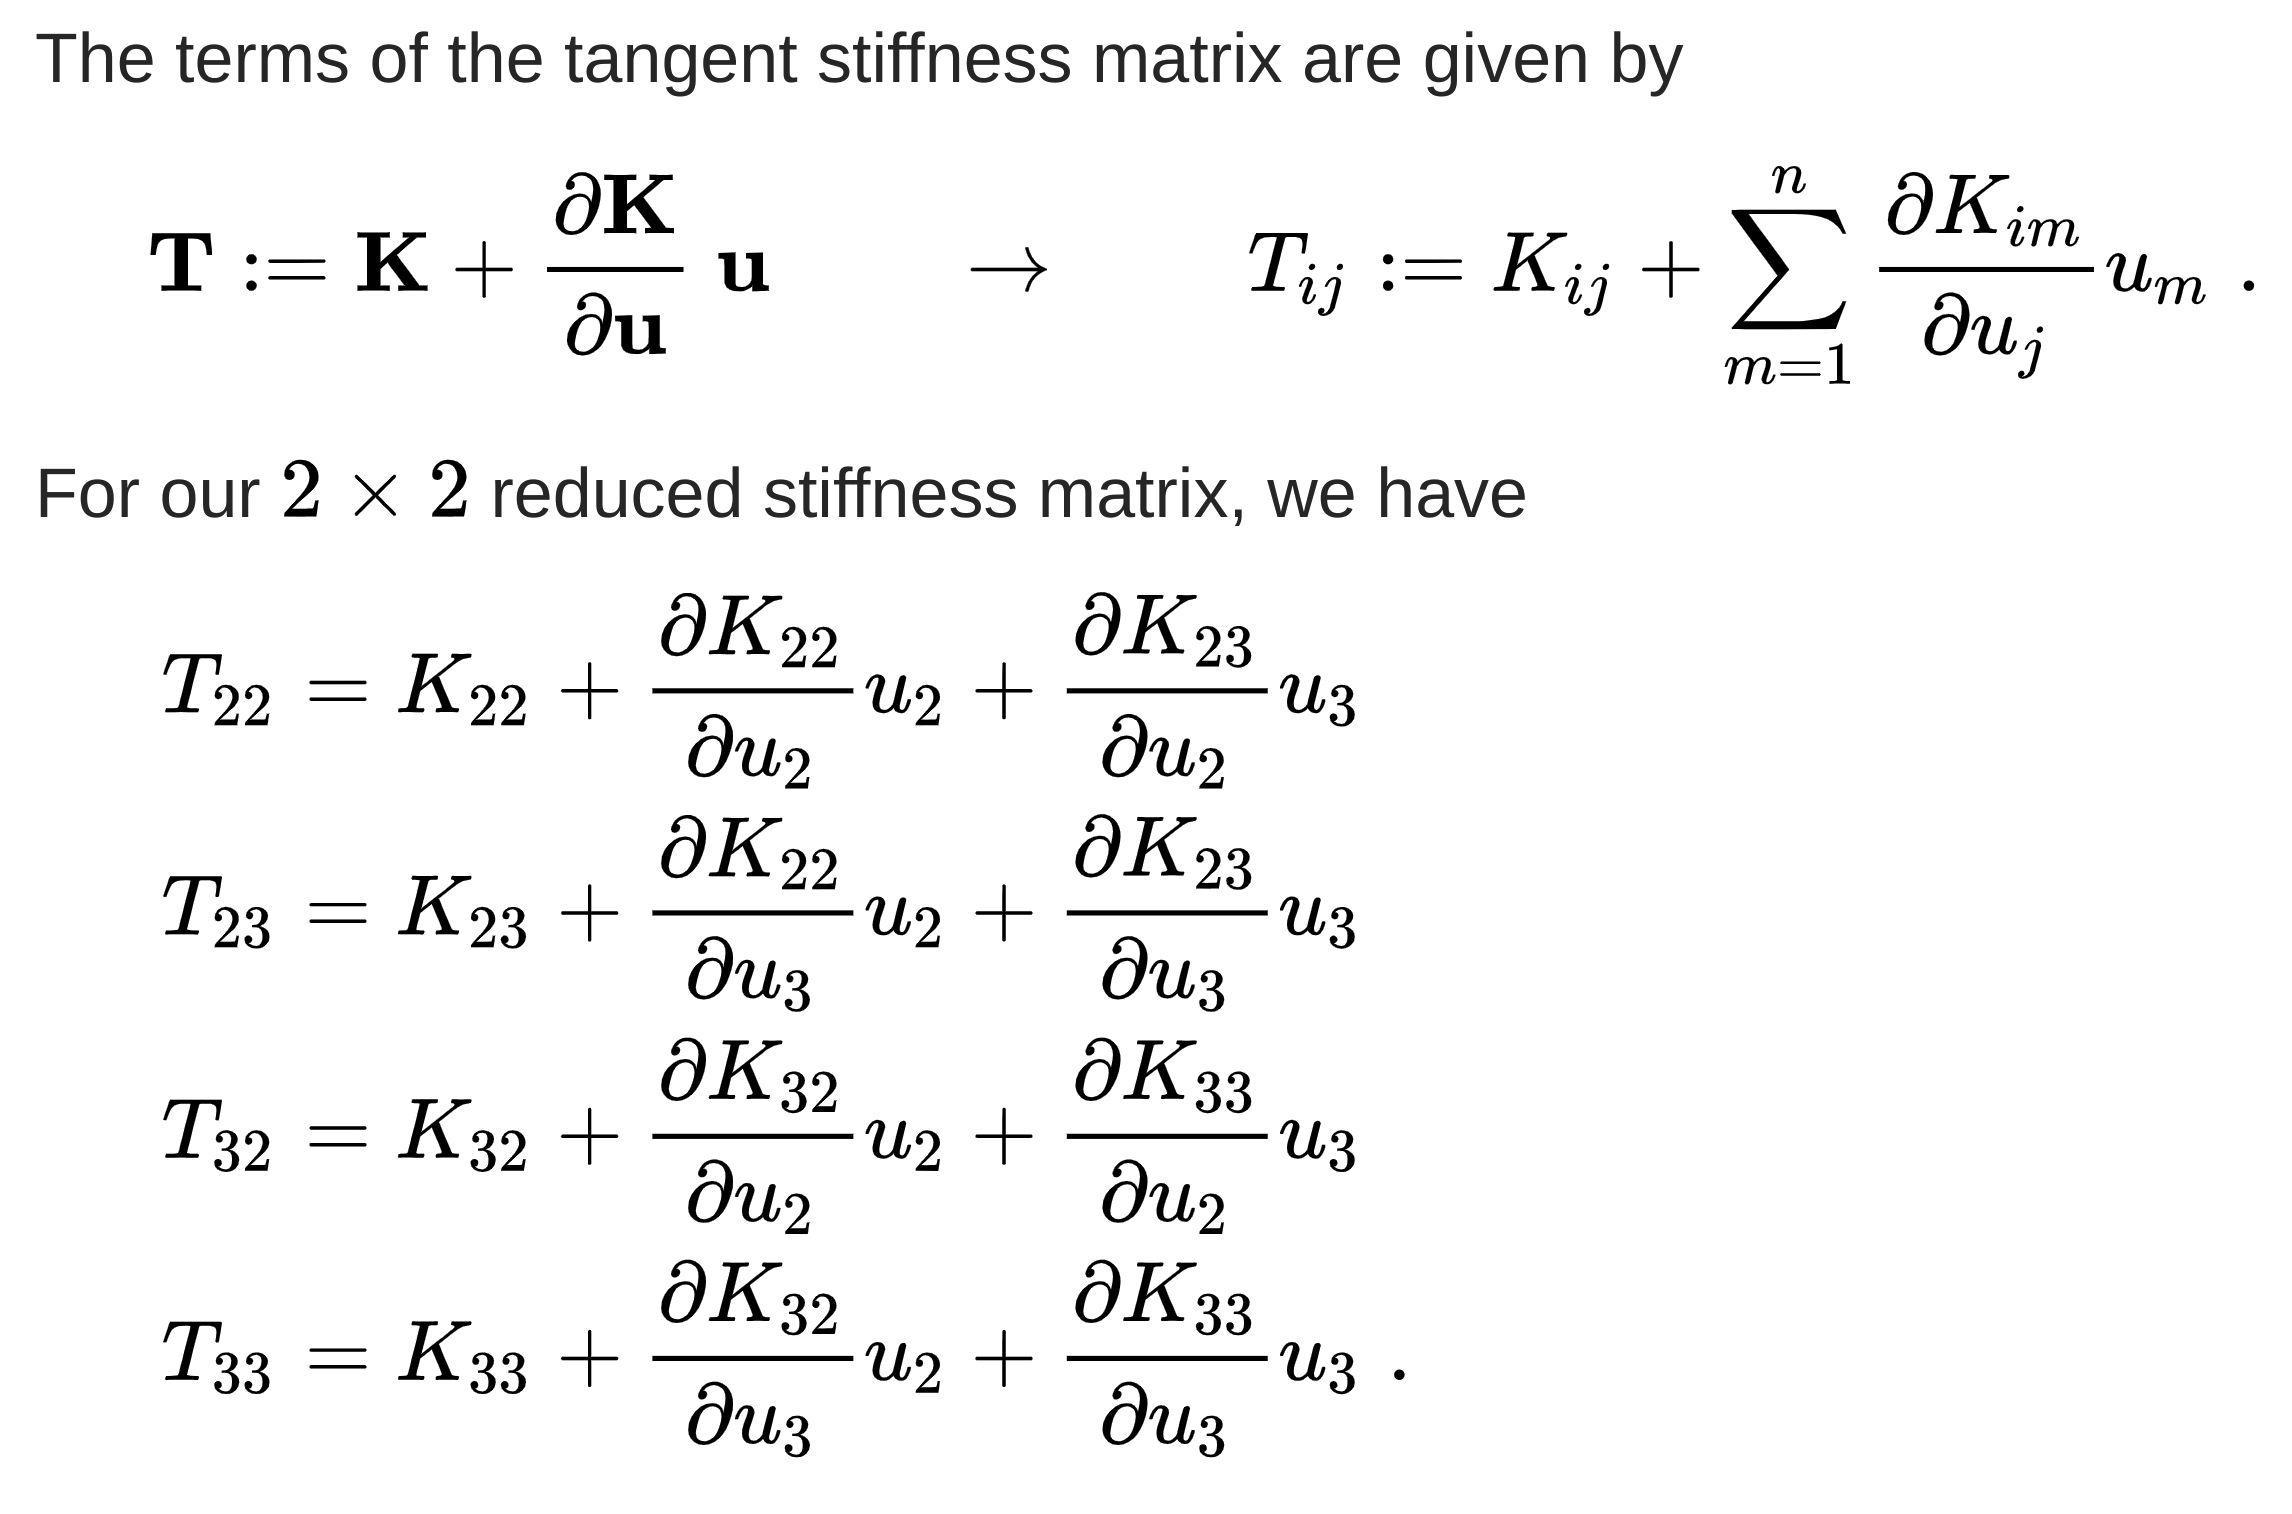
\includegraphics[width=\textwidth]{figs/tangent-matrix.png}
\end{figure}
\end{frame}


%------------------------------------------------
\begin{frame}
\frametitle{Newton Raphson iterative procedure: FE example}
The component definition of the tangent matrix at the element level is:
	\begin{equation*}
		\left[\mathbf{T({u})^r}\right] = K + \frac{\partial K}{\partial u} \rightarrow 
		\quad T_{ij} = K_{ij} + \sum_{m = 1}^n \frac{\partial K_{im}}{\partial u_j}u_m
	\end{equation*}

The residual vector after $r$ iteration is:
\mode<beamer>{
	\begin{equation*}
		{R({u}^{(r)})} = [K({u^r})]{u}^r - F
	\end{equation*}
The solution at $r+1$:
	\begin{equation*}
		{{u}^{(r+1)}} = {u}^r + {\delta u}	
	\end{equation*}
	\begin{equation*}
		{\delta \mathbf{u}}  = \left[\mathbf{T({u})^r}\right]^{-1} * {\mathbf{R({u^{r}})}}
	\end{equation*}
}
\mode<handout>{
	\vspace{4cm}
}
\end{frame}

%------------------------------------------------
\begin{frame}
\frametitle{Newton Raphson iterative procedure: FE example}
\begin{figure}[ht]
	\centering
	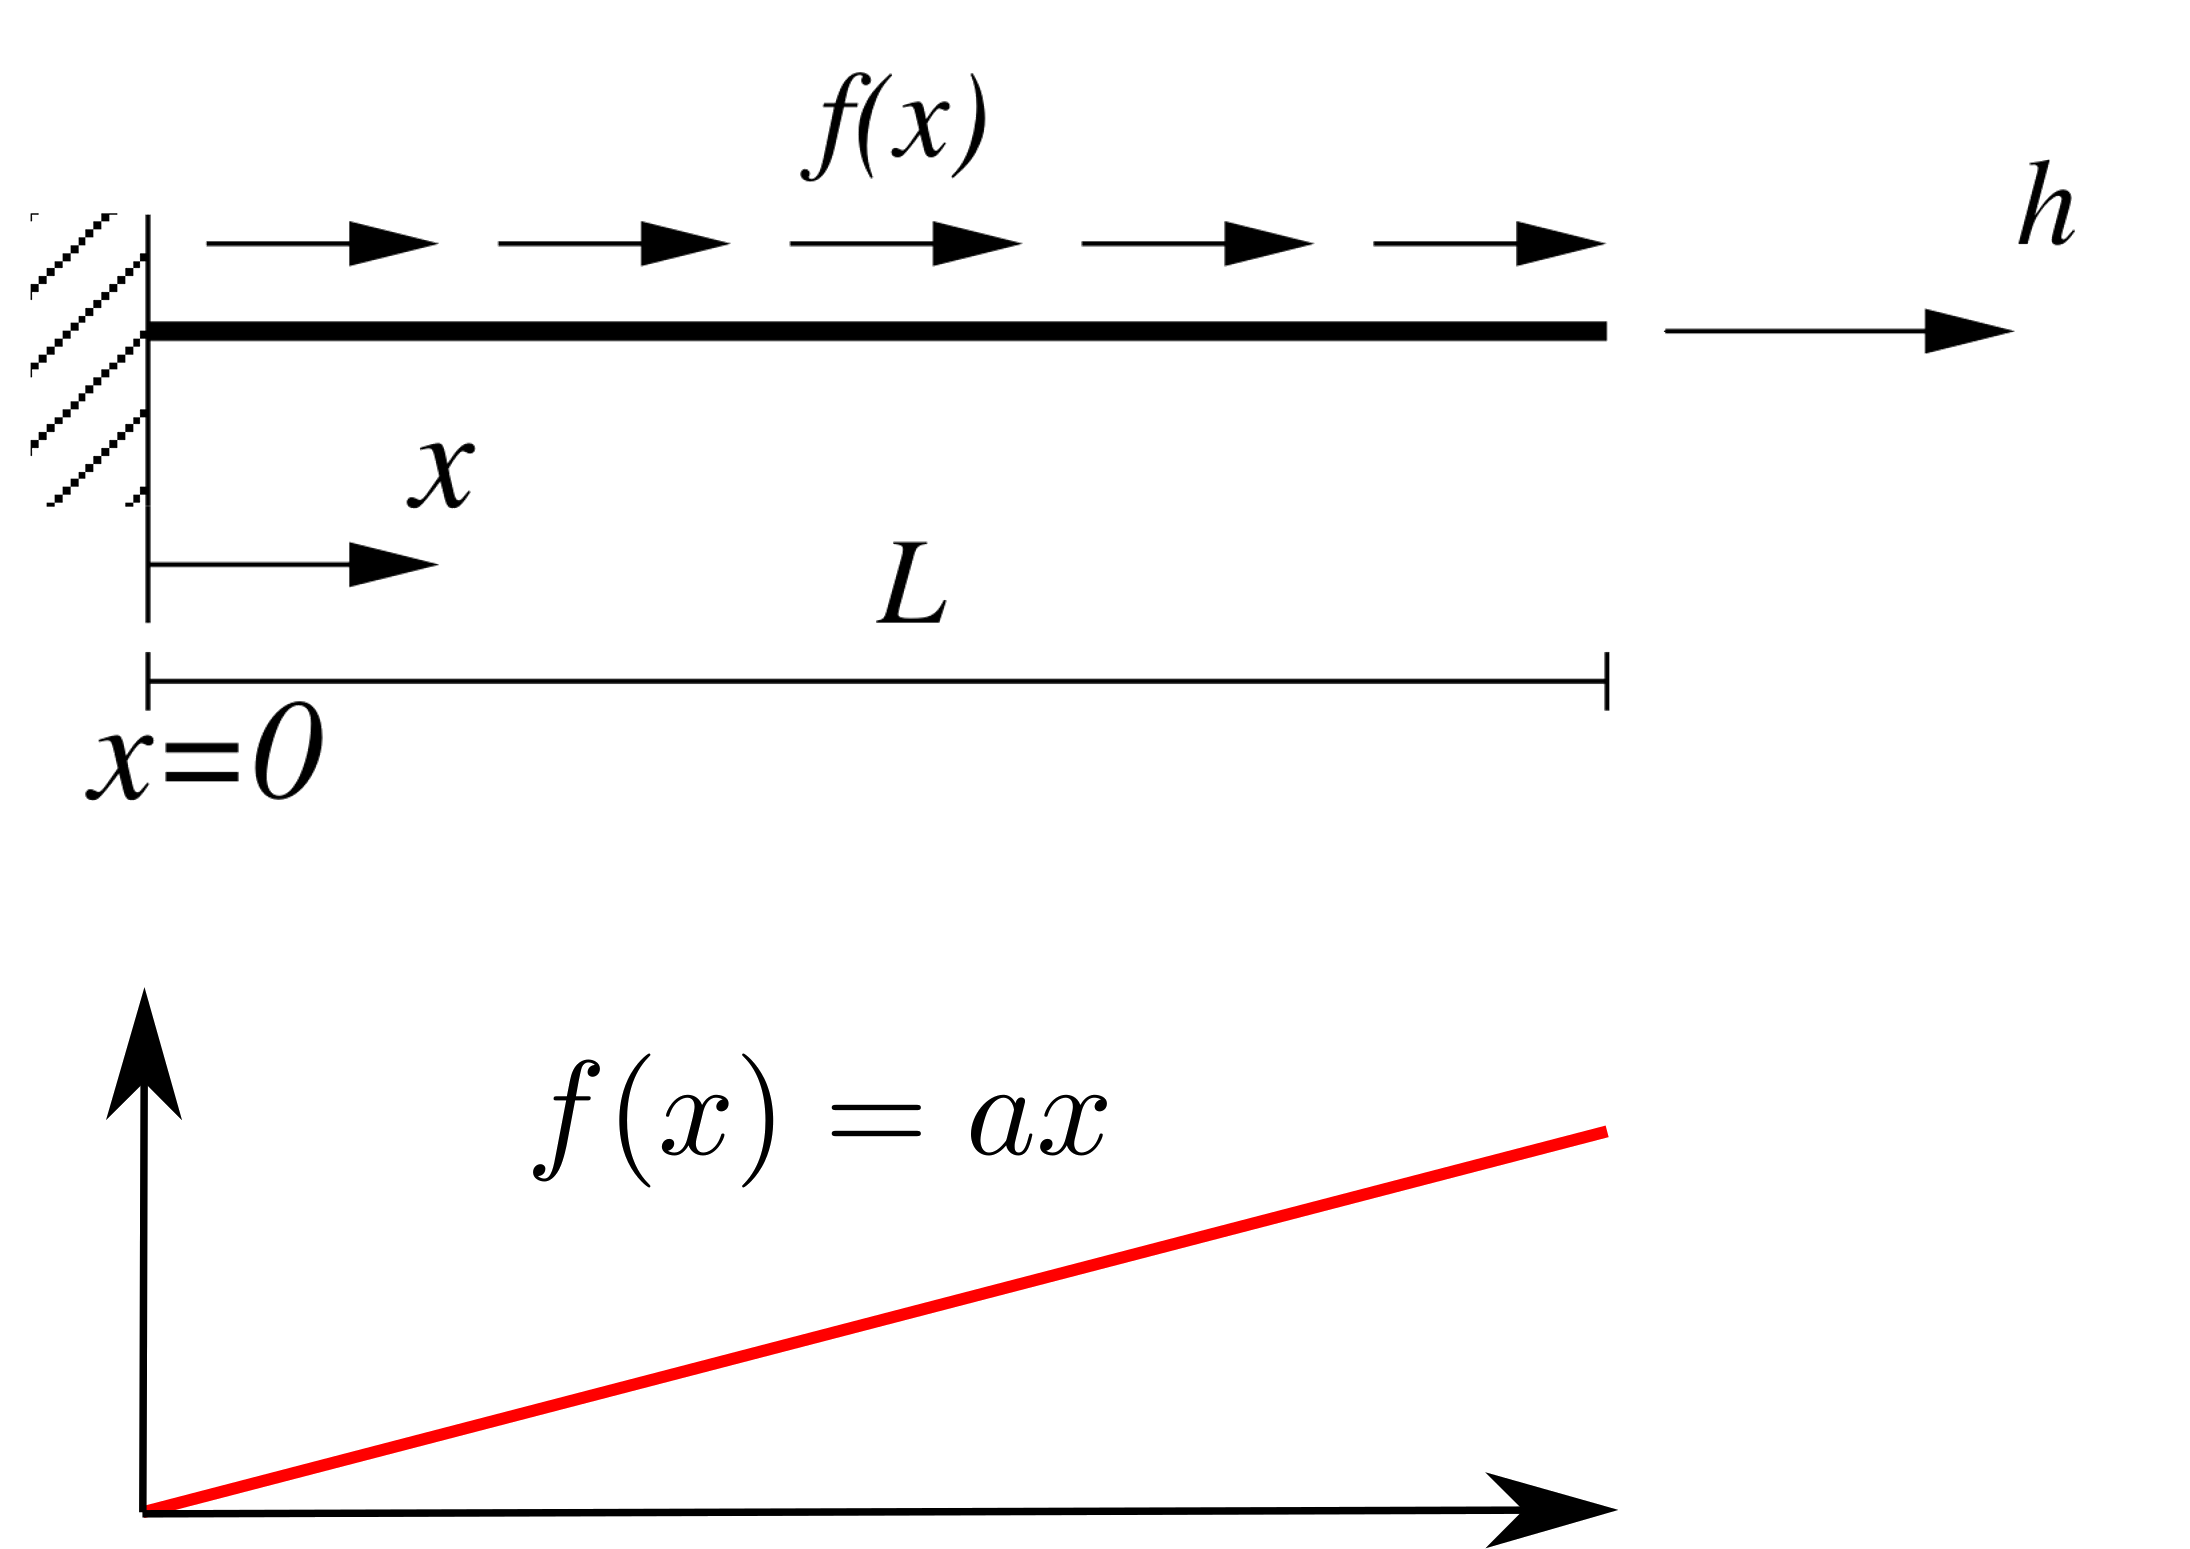
\includegraphics[width=0.7\textwidth]{figs/strong-form-nonlinear.png}
\end{figure}
The constitutive equation for this problem: $\sigma = E_0 (1 + \varepsilon)\varepsilon$
\end{frame}

%------------------------------------------------
\begin{frame}
\frametitle{Newton Raphson iterative procedure: FE example}
For the axial loading of a nonlinear bar:
\mode<beamer>{
	\begin{align*}
		-\frac{dN}{dx} & = f \\
		N & = g(\frac{du}{dx}) \\
		N & = AE\left(1 + \frac{du}{dx}\right)\frac{du}{dx}\\
	\end{align*}
}
\mode<handout>{
	\vspace{4cm}
}
The weakform:
\mode<beamer>{
	\begin{equation*}
	-\frac{d}{dx}\left(AE\left(1 + \frac{du}{dx}\right)\frac{du}{dx}\right) = f
	\end{equation*}
}
\mode<handout>{
	\vspace{3cm}
}
\end{frame}

%------------------------------------------------
\begin{frame}
\frametitle{Newton Raphson iterative procedure: FE example}
Multiplying the weak form by a weight function:
	\begin{equation*}
		-\int_0^L w \frac{d}{dx}\left(AE\left(1 + \frac{du}{dx}\right)\frac{du}{dx}\right) dx = \int_0^L wf dx
	\end{equation*}
Applying boundary condition (Dirichlet condition of $u(0) = 0$) and doing integration by parts:	
	\begin{equation*}
		-\int_0^L AE\left(1 + \frac{du}{dx}\right)\frac{du}{dx} \frac{dw}{dx} dx = \int_0^L wf dx
	\end{equation*}
\mode<handout>{
	\vspace{2cm}
}
\end{frame}

%------------------------------------------------
\begin{frame}
\frametitle{Newton Raphson iterative procedure: FE example}
	\begin{figure}[ht]
		\centering
		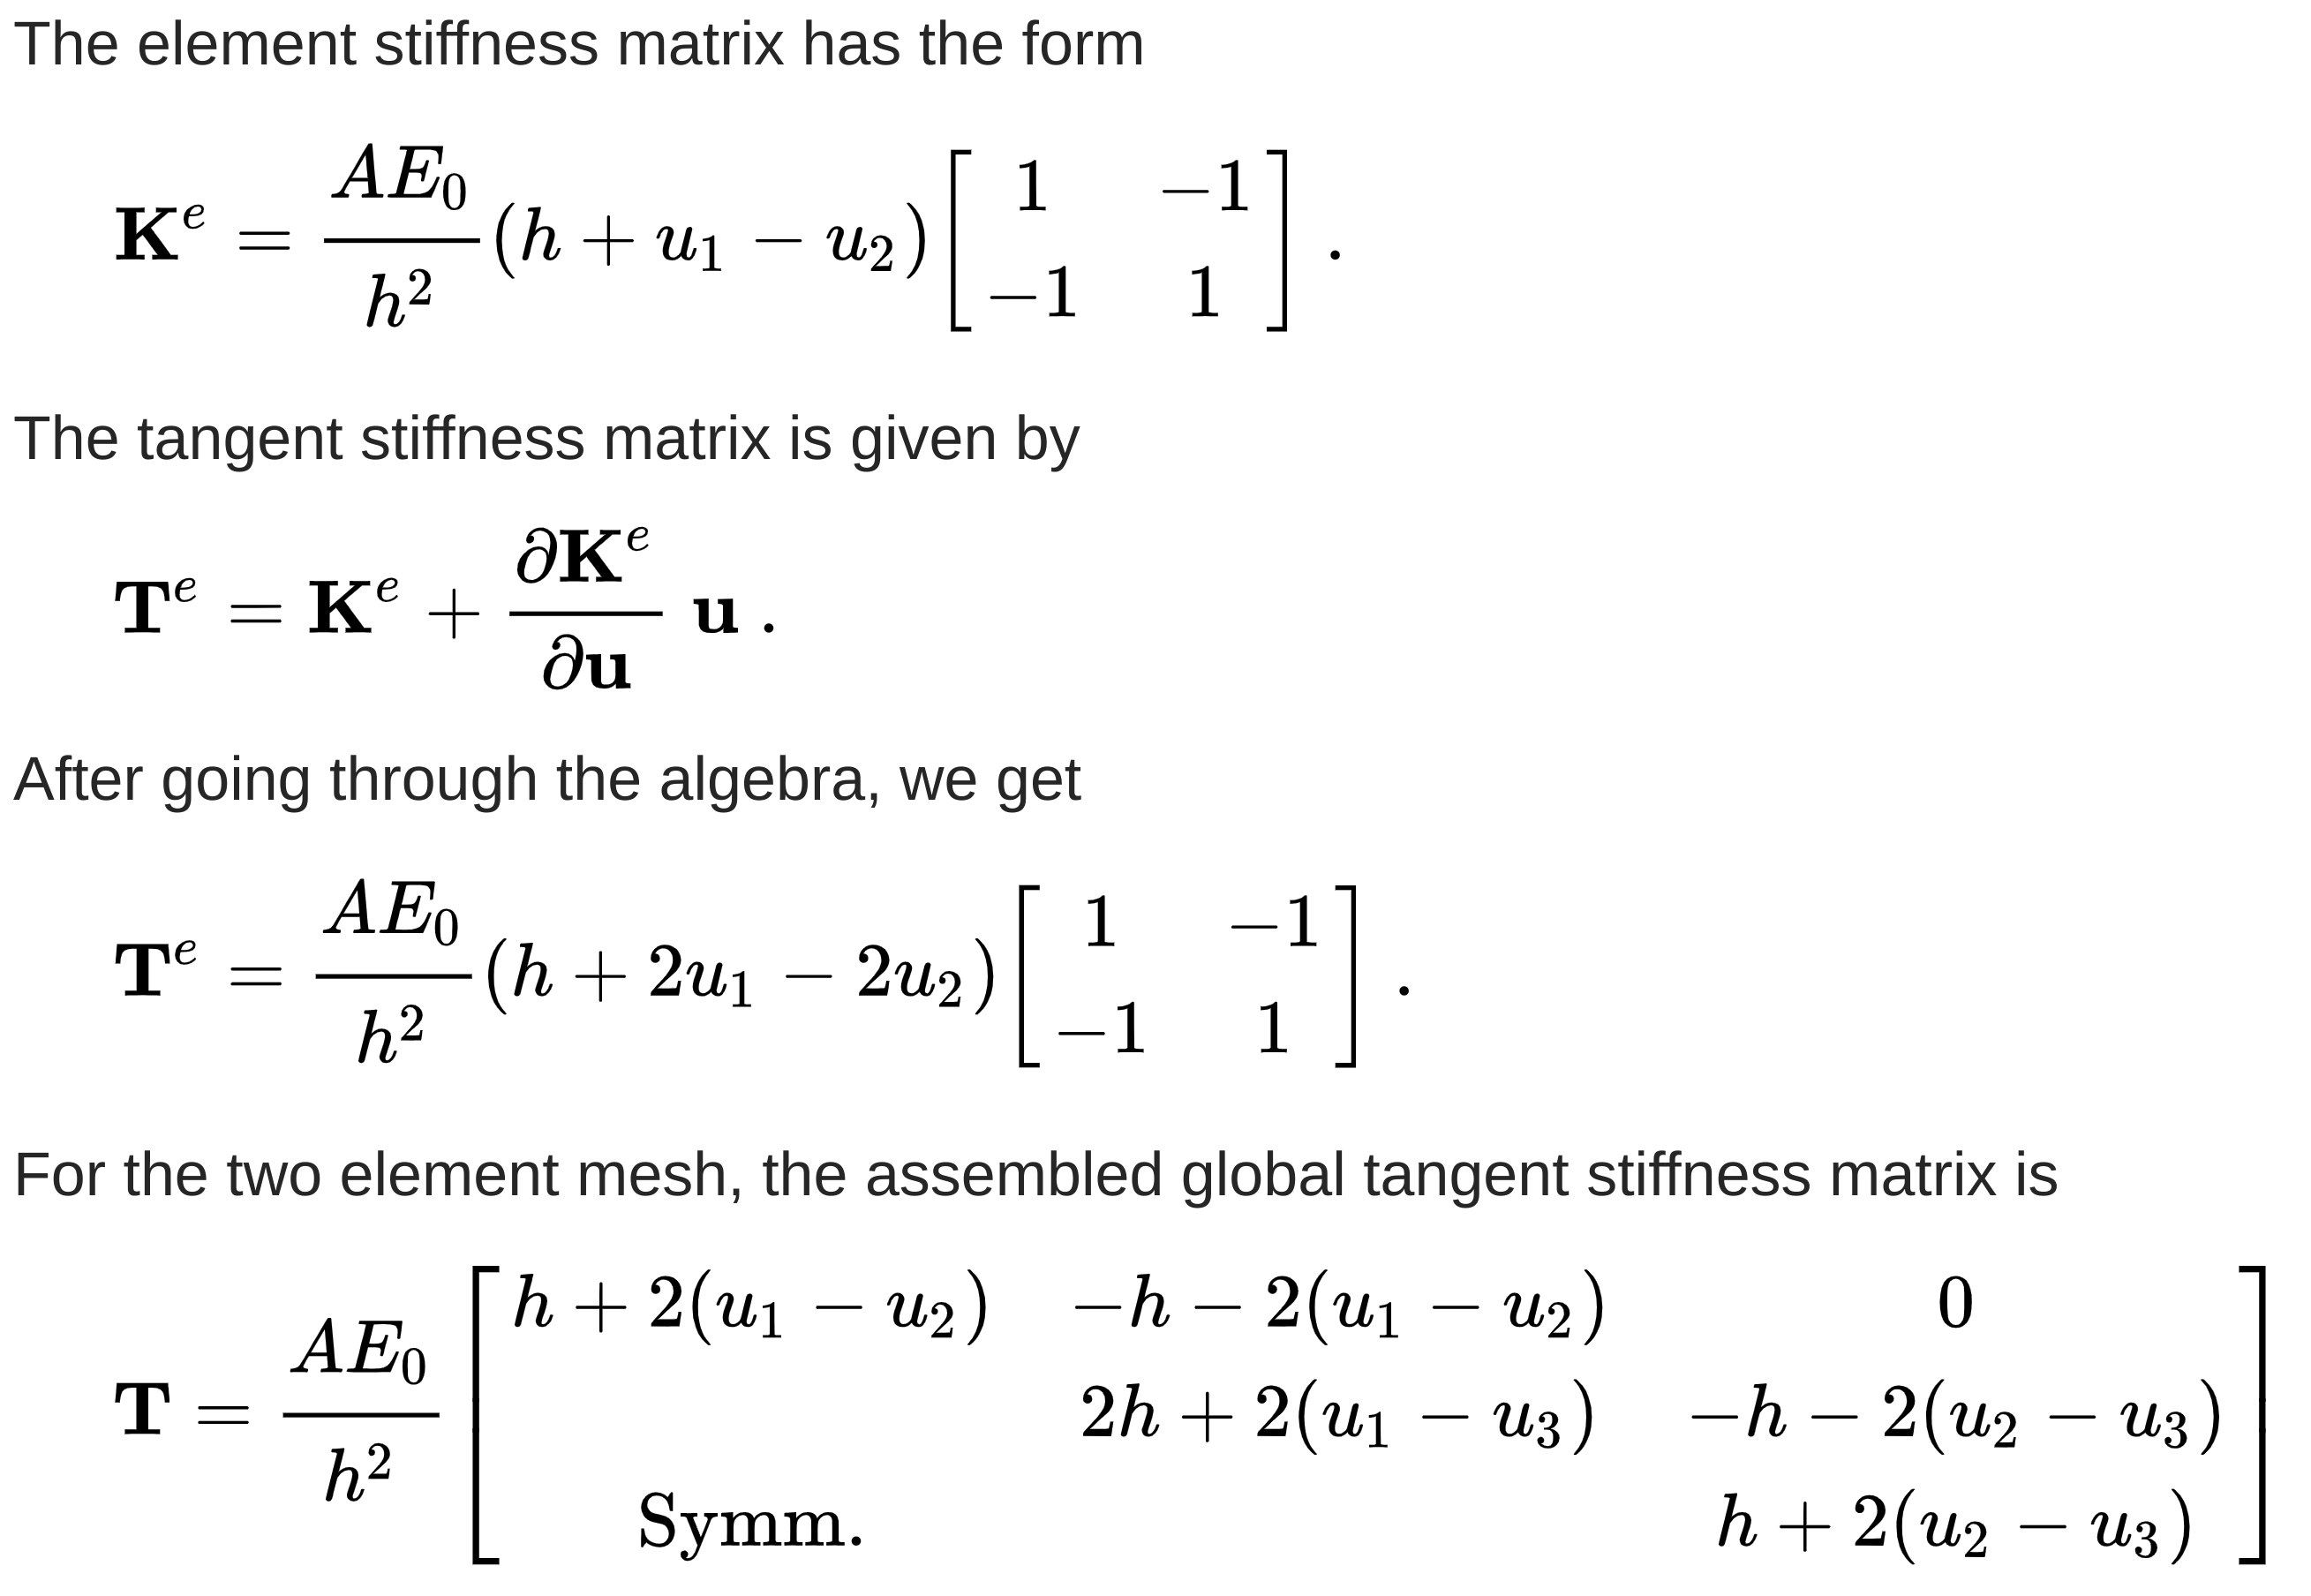
\includegraphics[width=0.9\textwidth]{figs/nonlinear-stiffness-matrix.png}
	\end{figure}
\end{frame}

%------------------------------------------------
\begin{frame}
\frametitle{Newton Raphson iterative procedure: FE example}
\begin{figure}[ht]
	\centering
	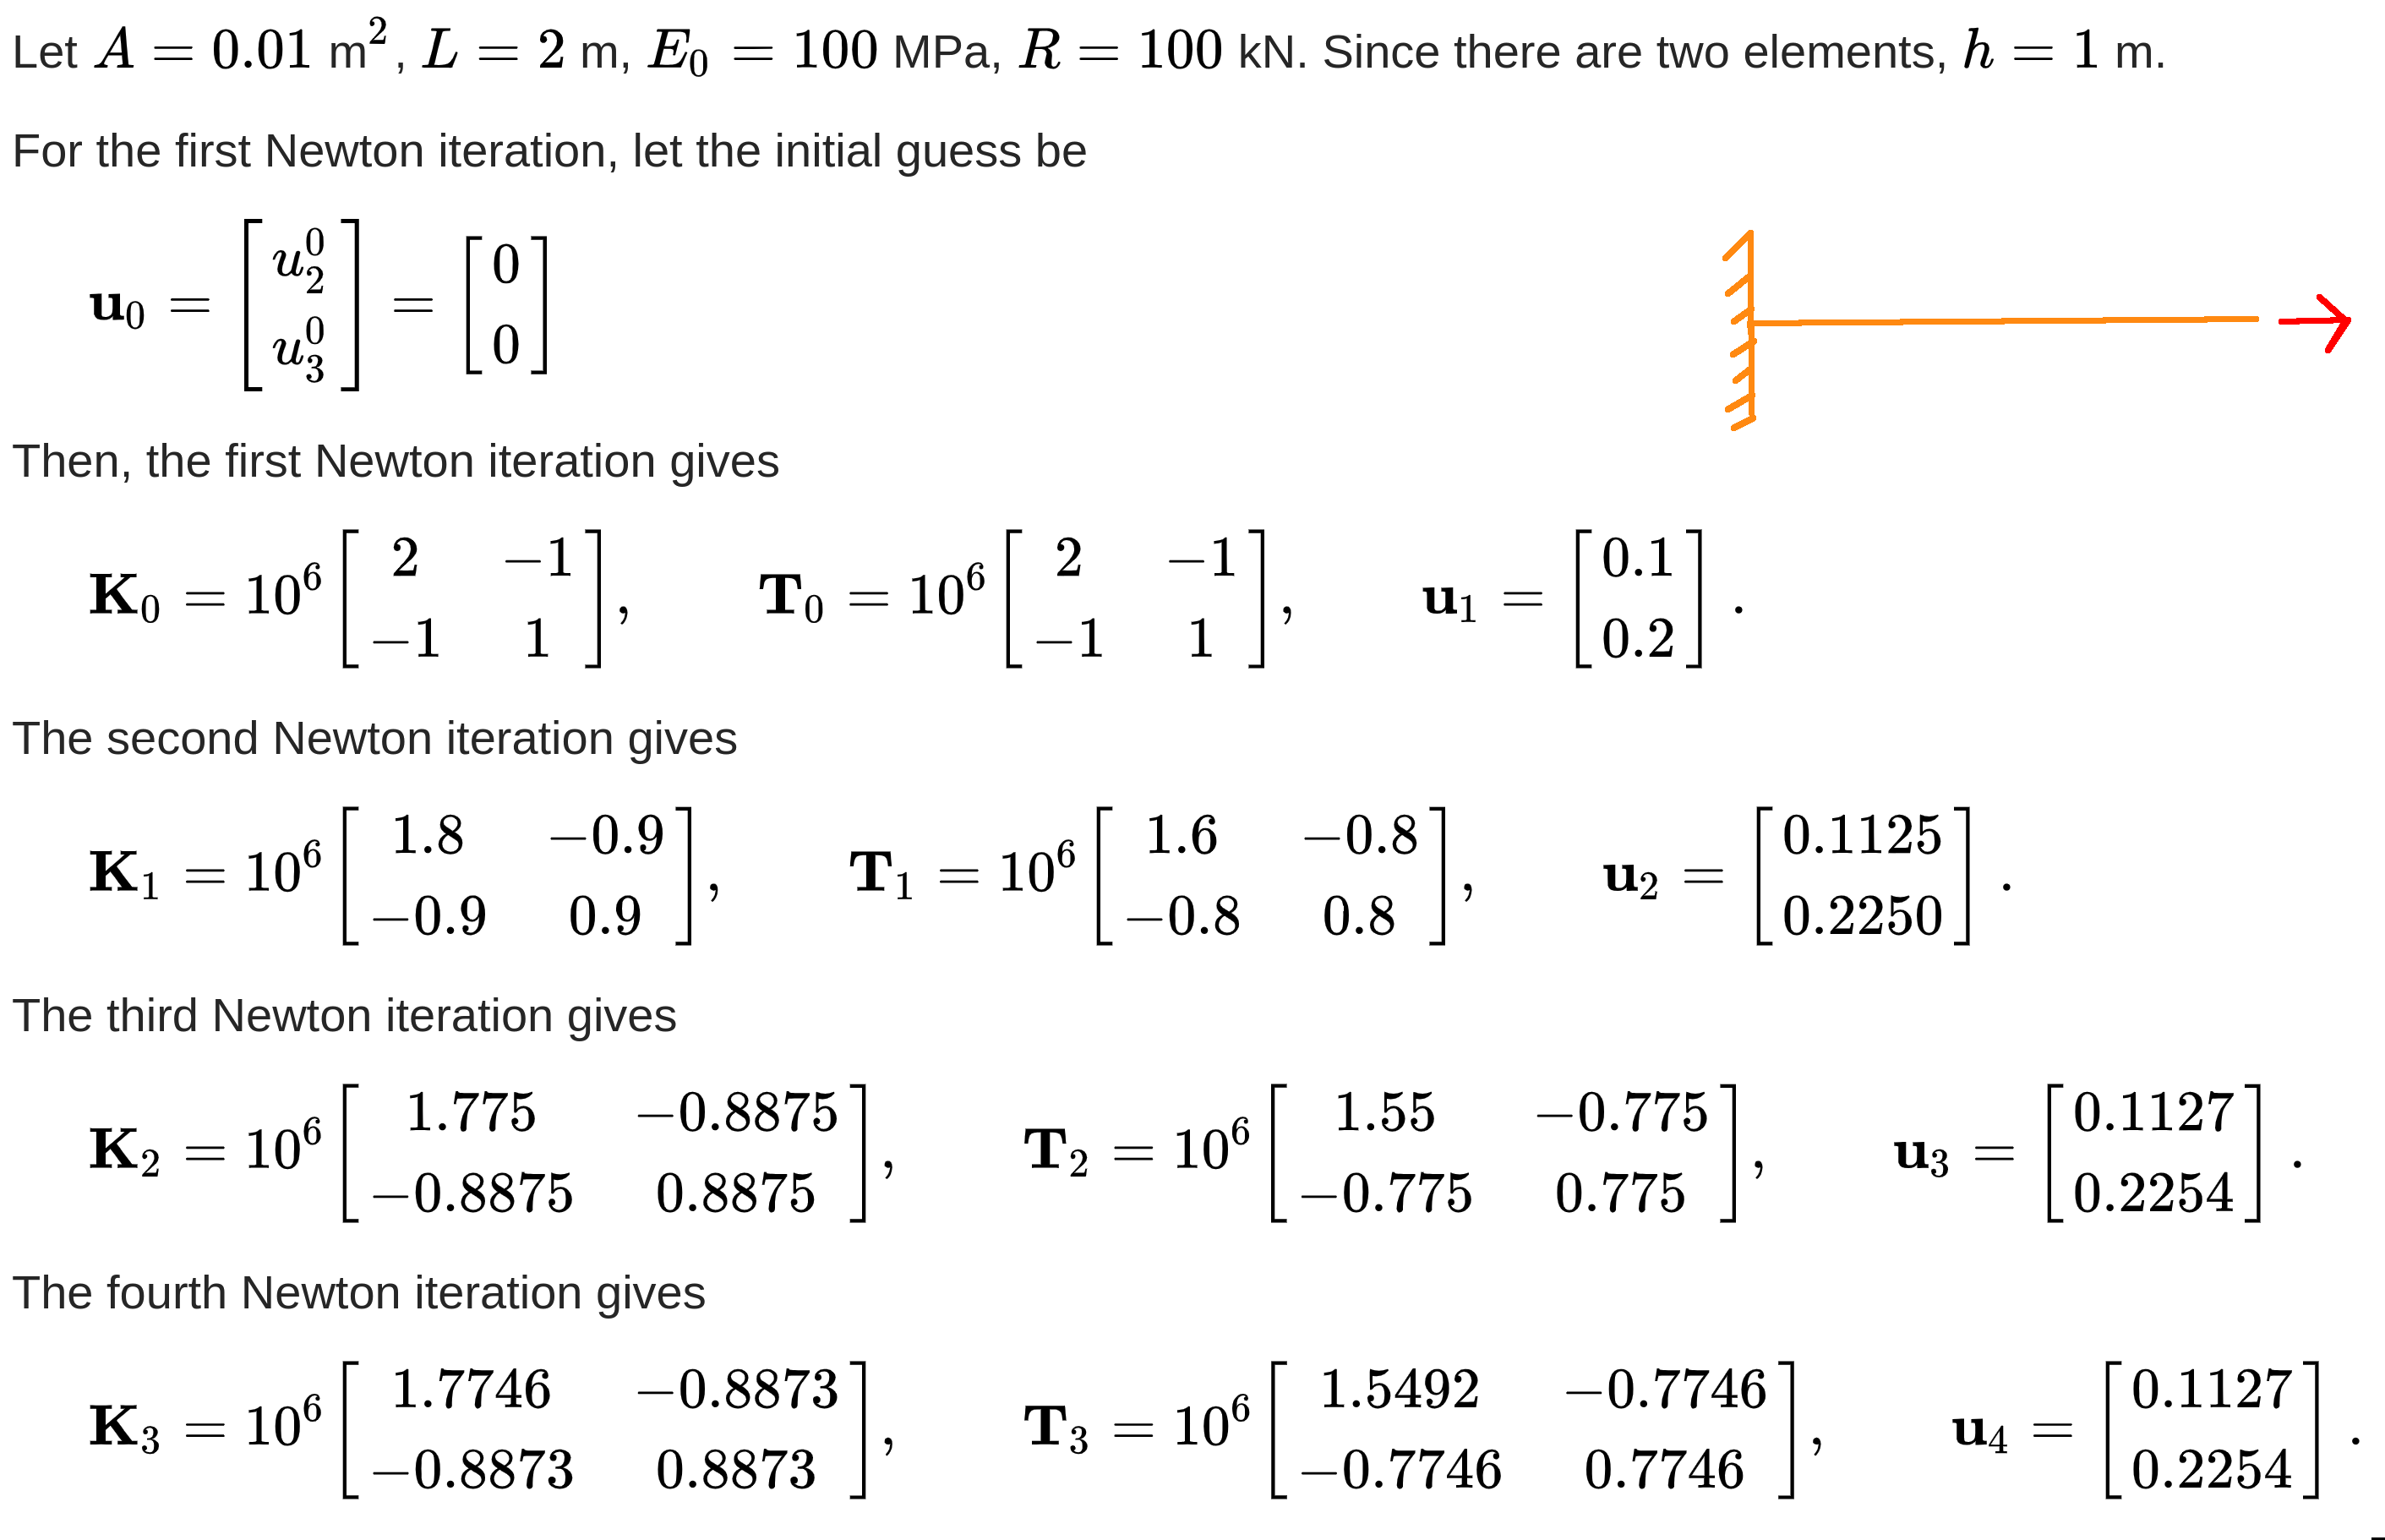
\includegraphics[width=0.9\textwidth]{figs/nr-nonlinear.png}
\end{figure}
\end{frame}

%------------------------------------------------
\begin{frame}
\frametitle{Newton Raphson iterative procedure: FE example}
\begin{figure}[ht]
	\centering
	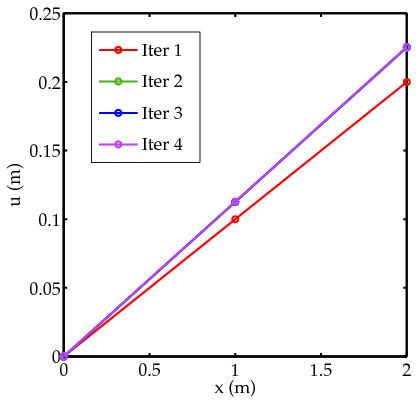
\includegraphics[width=0.65\textwidth]{figs/nr-linear.png}
\end{figure}
\end{frame}

%------------------------------------------------
\begin{frame}
\frametitle{Newton Raphson iterative procedure: FE example}
\begin{figure}[ht]
\centering
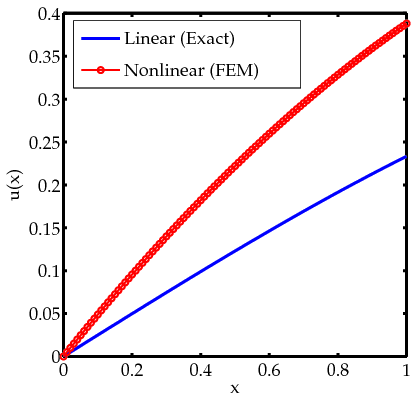
\includegraphics[width=0.6\textwidth]{figs/nr-linear-100.png}
\caption*{FEM displacement solution for nonlinear bar under distributed axial load. We have used 100 linear elements in these calculations.}
\end{figure}
\end{frame}

%------------------------------------------------
\begin{frame}
\frametitle{Newton Raphson: Drawbacks}
\mode<beamer>{
	\begin{figure}[ht]
		\centering
		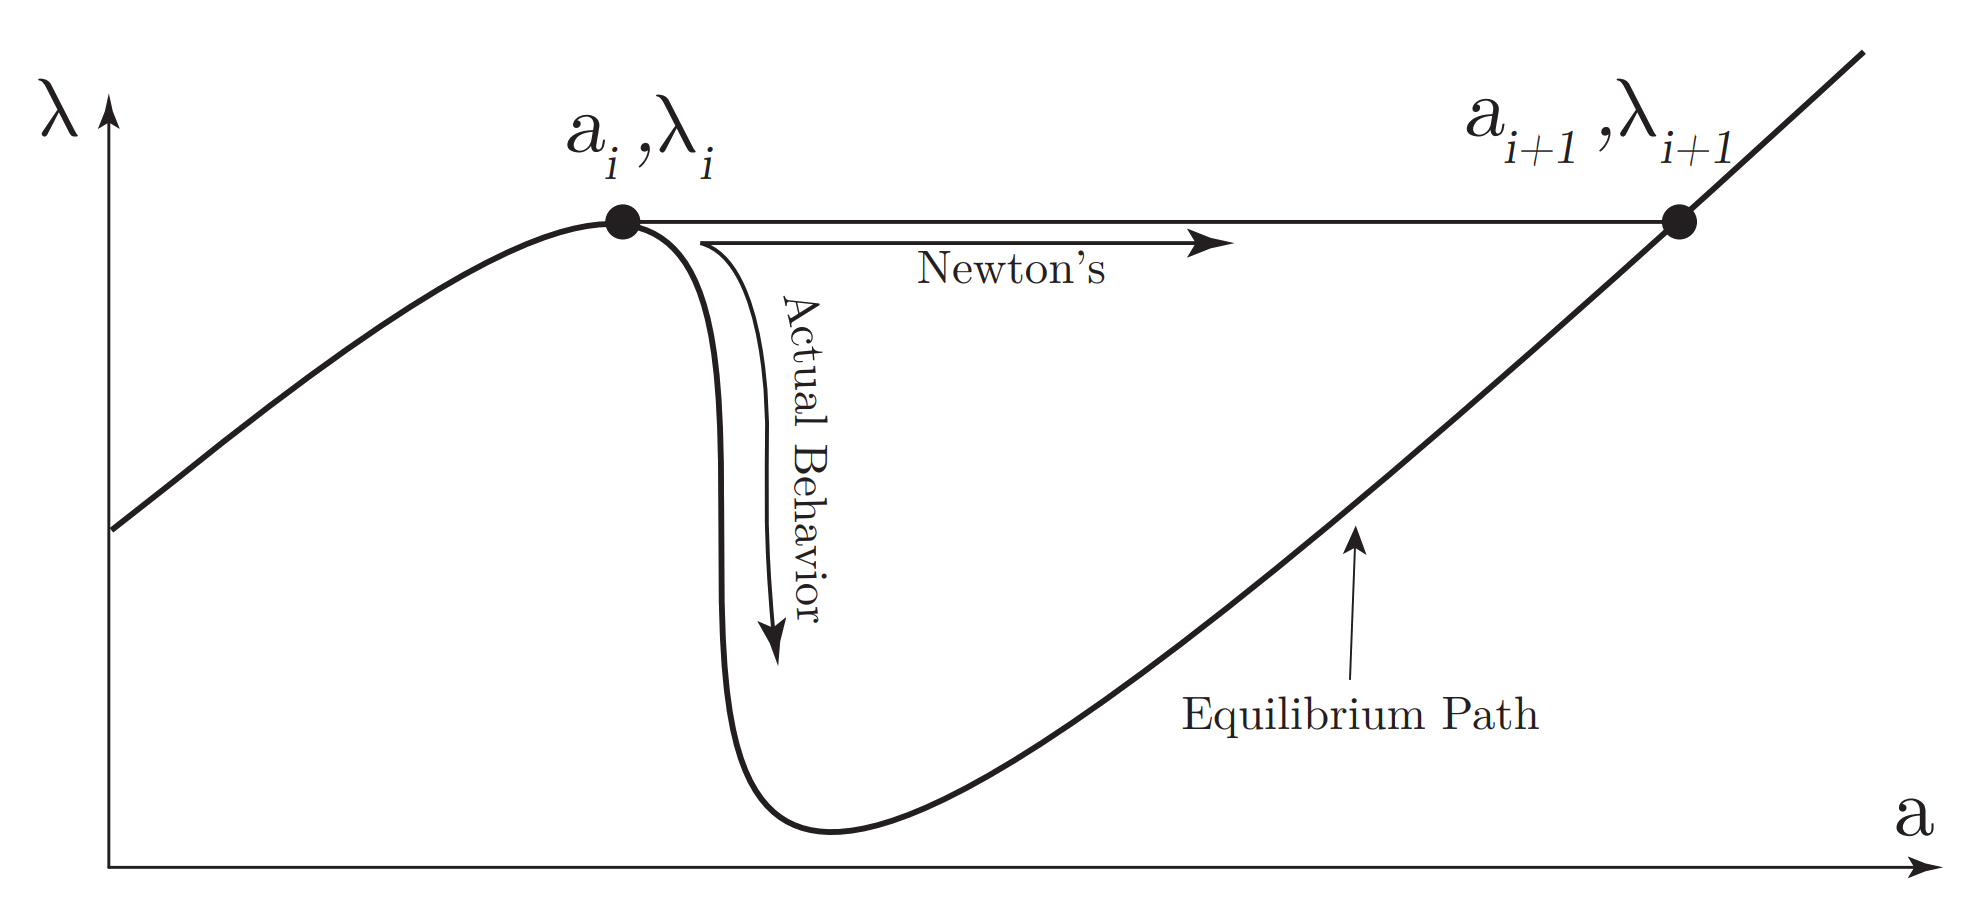
\includegraphics[width=\textwidth]{figs/newton-snap-through.png}
	\end{figure}
}
\mode<handout>{
	\vspace{6cm}
}
\end{frame}

\note{
	Newton's method fails to accurately follow the ‘equilibrium’ path once the tangent
	stiffness reaches zero. That happens due to the formulation of Newton’s method, and in particular that it
	restricts the parameter $\lambda$ to change monotonically every increment 3 . The definition of a limit point then (saddle points excluded), suggests that in order to remain on the equilibrium path you need to change your
	loading pattern depending on whether the limit point is a local maximum or maximum in the $u - \lambda$ space.
}

\note{
	In terms of mechanical systems then, this method is able to solve any non-linear system of equations
	very efficiently but only up to the critical point (if any). In the case shown in figure, Newton’s method
	fails in load–control. Now in many cases, one way to circumvent problems like these is to use displacement
	control, where you can continuously increase the displacements $u$ and still remain on the equilibrium curve.
	In general however, apart from Snap–Through behaviors under load control, a problem may exhibit Snap–
	Back behaviors under displacement control or even both. The main problem is, that in
	most actual applications, the structural response, and therefore the equilibrium path, for the structure under
	consideration is unknown, and therefore one does not know what type of behavior to expect.
}
\note{
	 As a general
	rule, if the problem under consideration requires information after its critical/failure points then Newton’s
	method is not a good choice. Buckling analysis and non-linear materials that exhibit work softening are
	just two example problems that cannot be solved using Newton’s method. Furthermore, very often, strong
	nonlinearities that arise in finite deformation problems may eventually lead to such behaviors and thus it is
	necessary to introduce a numerical technique to solve such problem with strongly nonlinear behaviors.
}


%------------------------------------------------
\begin{frame}
\frametitle{Newton Raphson: Drawbacks}
\mode<beamer>{
	\begin{figure}[ht]
		\centering
		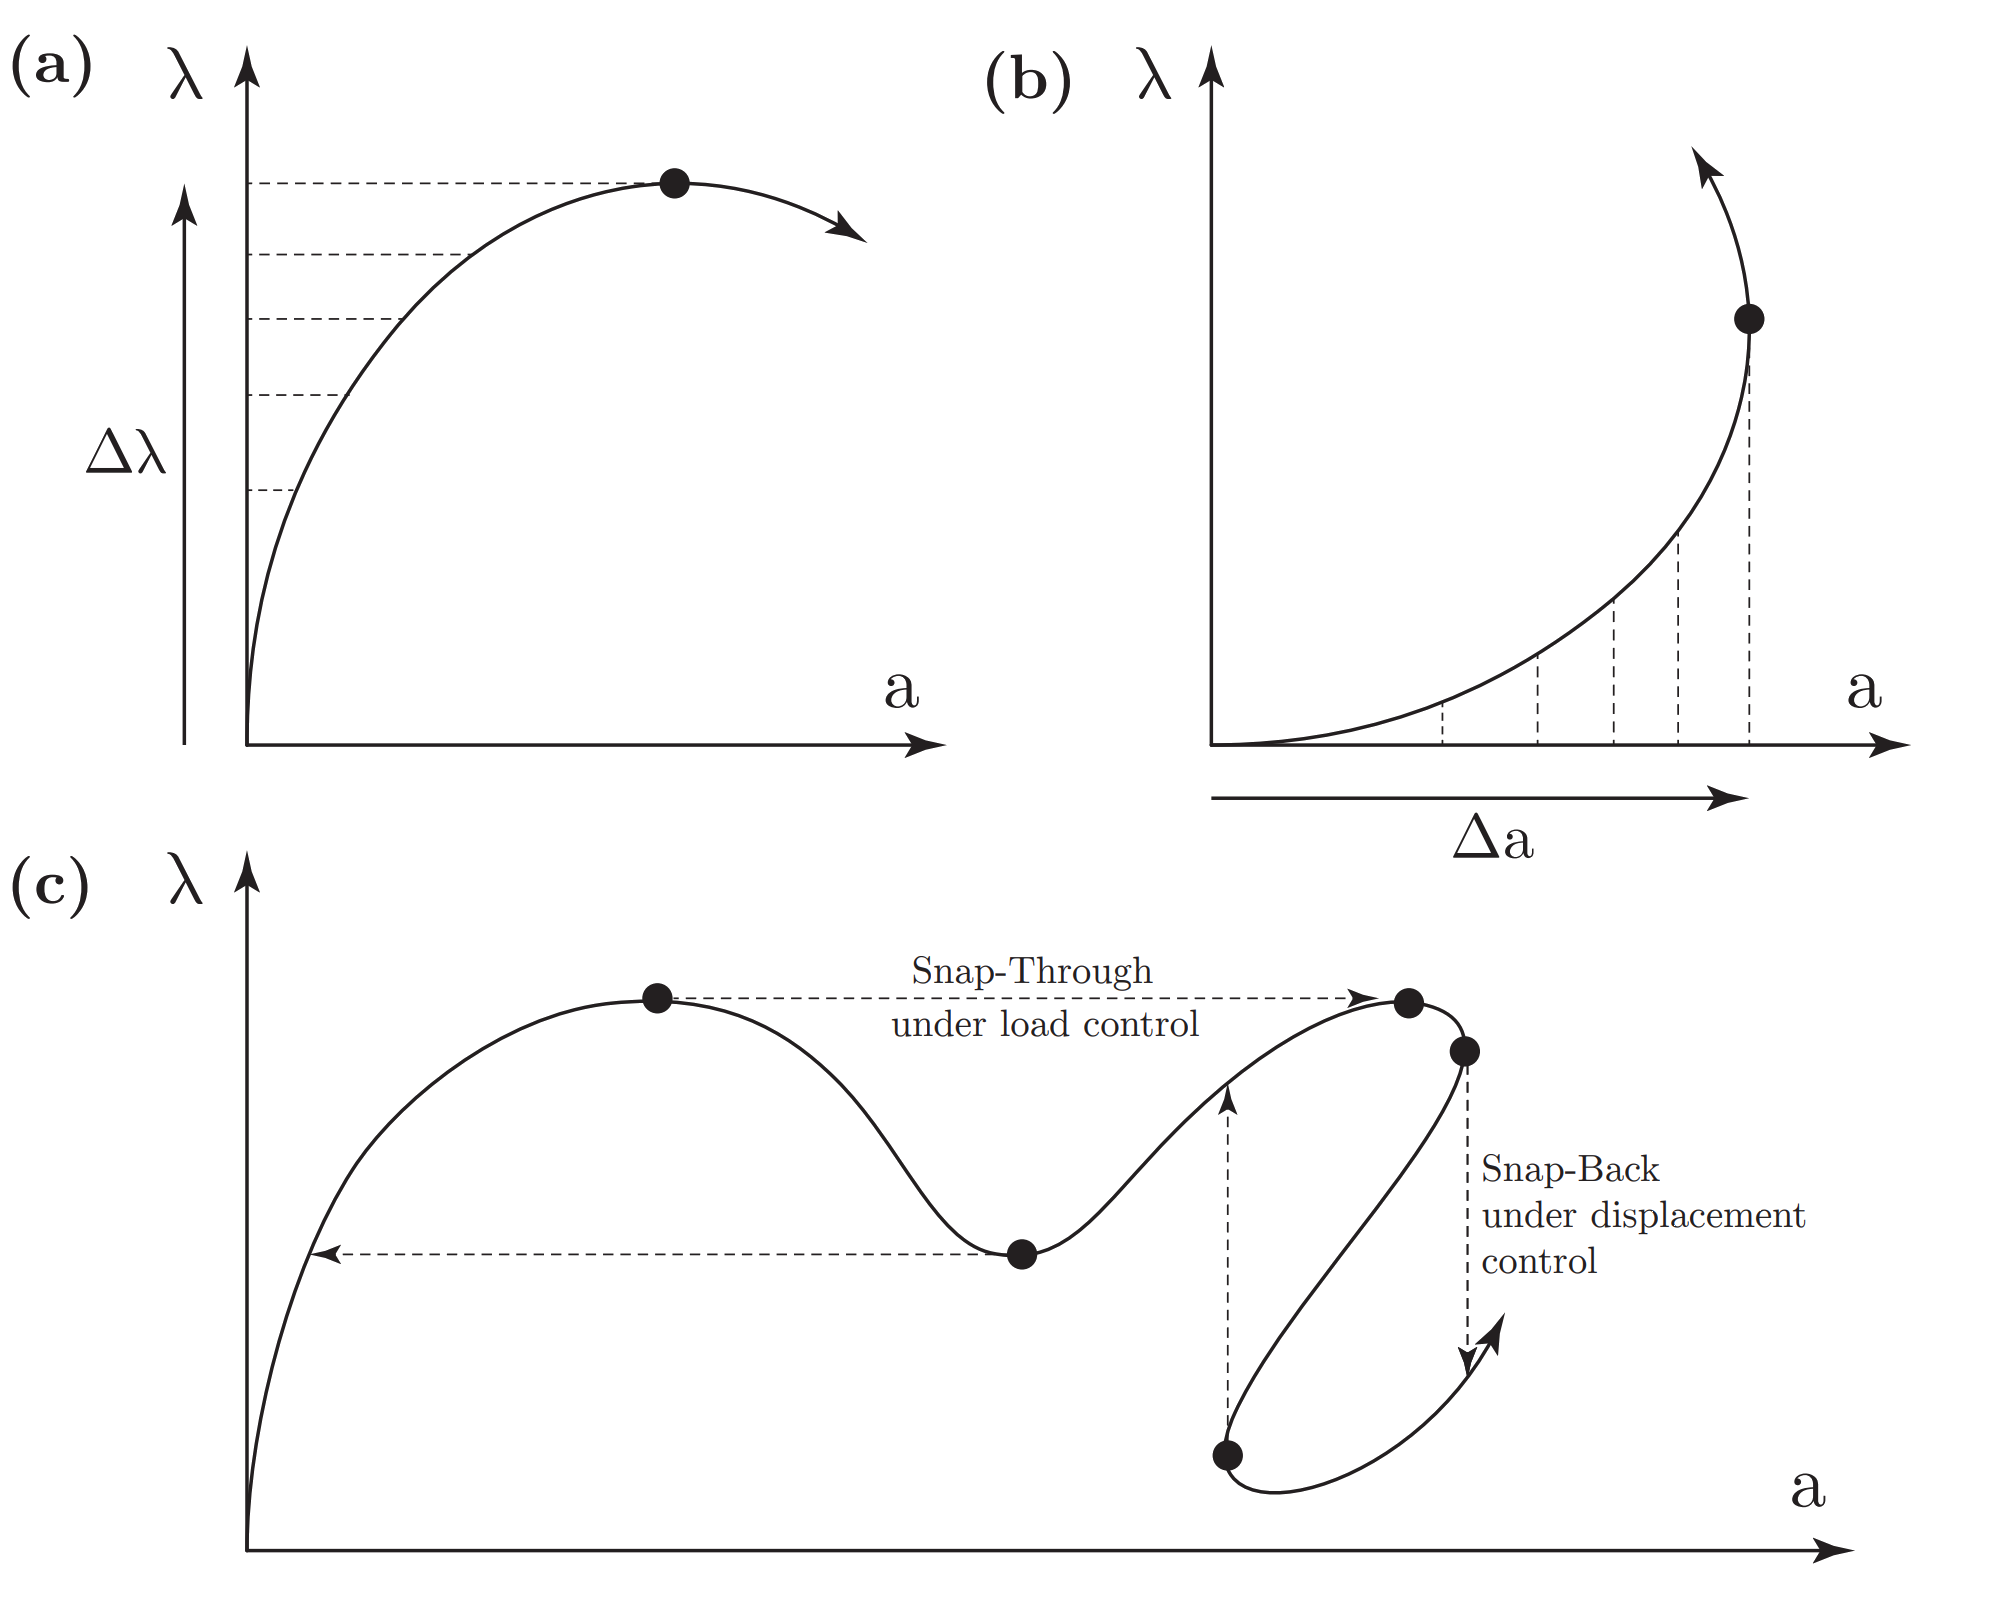
\includegraphics[width=0.65\textwidth]{figs/newton-failures.png}
		\caption*{(a) A system that is unstable under load control (Snap–Through instability), (b) A system that is unstable under displacement control (Snap–Back Instability), (c) A system that is unstable under both displacement and load control}
	\end{figure}
}
\mode<handout>{
	\vspace{6cm}
}
\end{frame}

\section{Arc length method}
%------------------------------------------------
\begin{frame}
\frametitle{Arc length method}
System of the non-linear (in general) equations to solve:
\begin{equation*}
	F_{\mathrm{int}} - F_{\mathrm{ext}} = 0 \rightarrow F_{\mathrm{int}} - \lambda q = 0
\end{equation*}

Suppose ($u_0, \lambda_0$) satisfy the system of equations and thus belongs to the `equilibrium path'. Arc Length postulates a simultaneous variation in both the displacements $\Delta u$ and the load vector coefficient $\Delta \lambda$.

\mode<beamer>{
\begin{equation*}
	R(u^\prime, \lambda^\prime) = F_{\mathrm{int}}(u_0 + \Delta u) - (\lambda_0 + \Delta \lambda)q = 0
\end{equation*}


If the above is satisfied for $(u_0 + \Delta u, \lambda_0 + \Delta \lambda)$ then this point also belongs to the ‘equilibrium path’ and we can successfully update the solution. However, immediate satisfaction is not possible, so we need to provide the necessary corrections $(\delta u, \delta \lambda)$, aiming that the new point $(u_0 + \Delta u + \delta u, \lambda_0 + \Delta \lambda + \delta \lambda)$ will satisfy. 


	\begin{equation*}
		R(u^{\prime \prime}, \lambda^{\prime \prime}) = F_{\mathrm{int}}(u_0 + \Delta u + \delta u) - (\lambda_0 + \Delta \lambda+ \delta \lambda)q = 0
	\end{equation*}
	
}
\mode<handout>{
	\vspace{4cm}
}
\end{frame}


\note{
	Arc length is a very efficient method in solving non-linear systems of equations when the problem under consideration exhibits one or more critical points. In terms of a simple mechanical
	loading-unloading problem, a critical point could be interpreted as the point at which the loaded body
	cannot support an increase of the external forces and an instability occurs.\\
	
	Unlike the Newton-Method, the Arc Length method postulates a
	simultaneous variation in both the displacements $\Delta u$ and the load vector coefficient $\Delta \lambda$. The main difference is that both $\Delta u$ and $\Delta \lambda$ are unknowns in contrast to Newton’s method where  $\Delta \lambda$ was given and we had to iteratively solve for $\Delta u$.
}

\note {
	The system of equations takes the form:
	\begin{equation*}
		\left[K^T \right]_{u_0 + \Delta u} \cdot \delta u - \delta \lambda q = - \left[F_{\mathrm{int}}(u_0 + \Delta u) - (\lambda_0 + \Delta \lambda) q \right] = - R (u^\prime, \lambda^\prime)		
	\end{equation*}
	$\delta u$ and $\delta lambda$ are the unknowns for whom we need to solve. If the $u$ vector however, has dimensions 	$N \times 1$ then we have a total of $N$ equations that we need to solve for $N+1$ unknowns ($N$ unknowns $\delta u$ and 1 unknown $\delta \lambda$). Equations then are not sufficient to determine $\delta u, \delta \lambda$. The supplementary equation that completes the system is called the Arc Length Equation.
	

}

%------------------------------------------------
\begin{frame}
\frametitle{Arc length method}
The Arc length equation:
	\begin{equation*}
		(\Delta \mathbf{u} + \delta \mathbf{u})^T \cdot (\Delta \mathbf{u} + \delta \mathbf{u}) + \psi^2 (\Delta \lambda + \delta \lambda)^2 (\mathbf{q}^T \cdot \mathbf{q}) = \Delta l^2
	\end{equation*}

where $\psi$ and $\Delta l$ are user defined parameters. In a sense $\Delta l$ defines how far to search for the next equilibrium point and it is analogous (but not directly equivalent) to the load increment $\Delta \lambda$ we used in Newton’s method.

\end{frame}

\note {The system of equations is solved for $\delta u, \delta \lambda$ and updates the previous corrections $\Delta u, \Delta \lambda$ to be $\Delta u^\prime = \Delta u + \delta u$ and $\Delta \lambda^\prime = \Delta \lambda + \delta \lambda$ respectively. The method continues to provide such incremental corrections $\delta u, \delta \lambda$ until convergence is achieved. When $\psi = 1$, the method is also called the \textbf{Spherical Arc-Length Method } because the points $\Delta u^\prime, \Delta \lambda^\prime$ belong to a circle with radius $\Delta l$. In its most general form for arbitrary $\psi$ can be geometrically interpreted as a hyper-ellipse in the multidimensional displacement-load space ($u - \lambda$).}


%------------------------------------------------
\begin{frame}
\frametitle{Arc length method}
\mode<beamer>{
	\begin{figure}[ht]
		\centering
		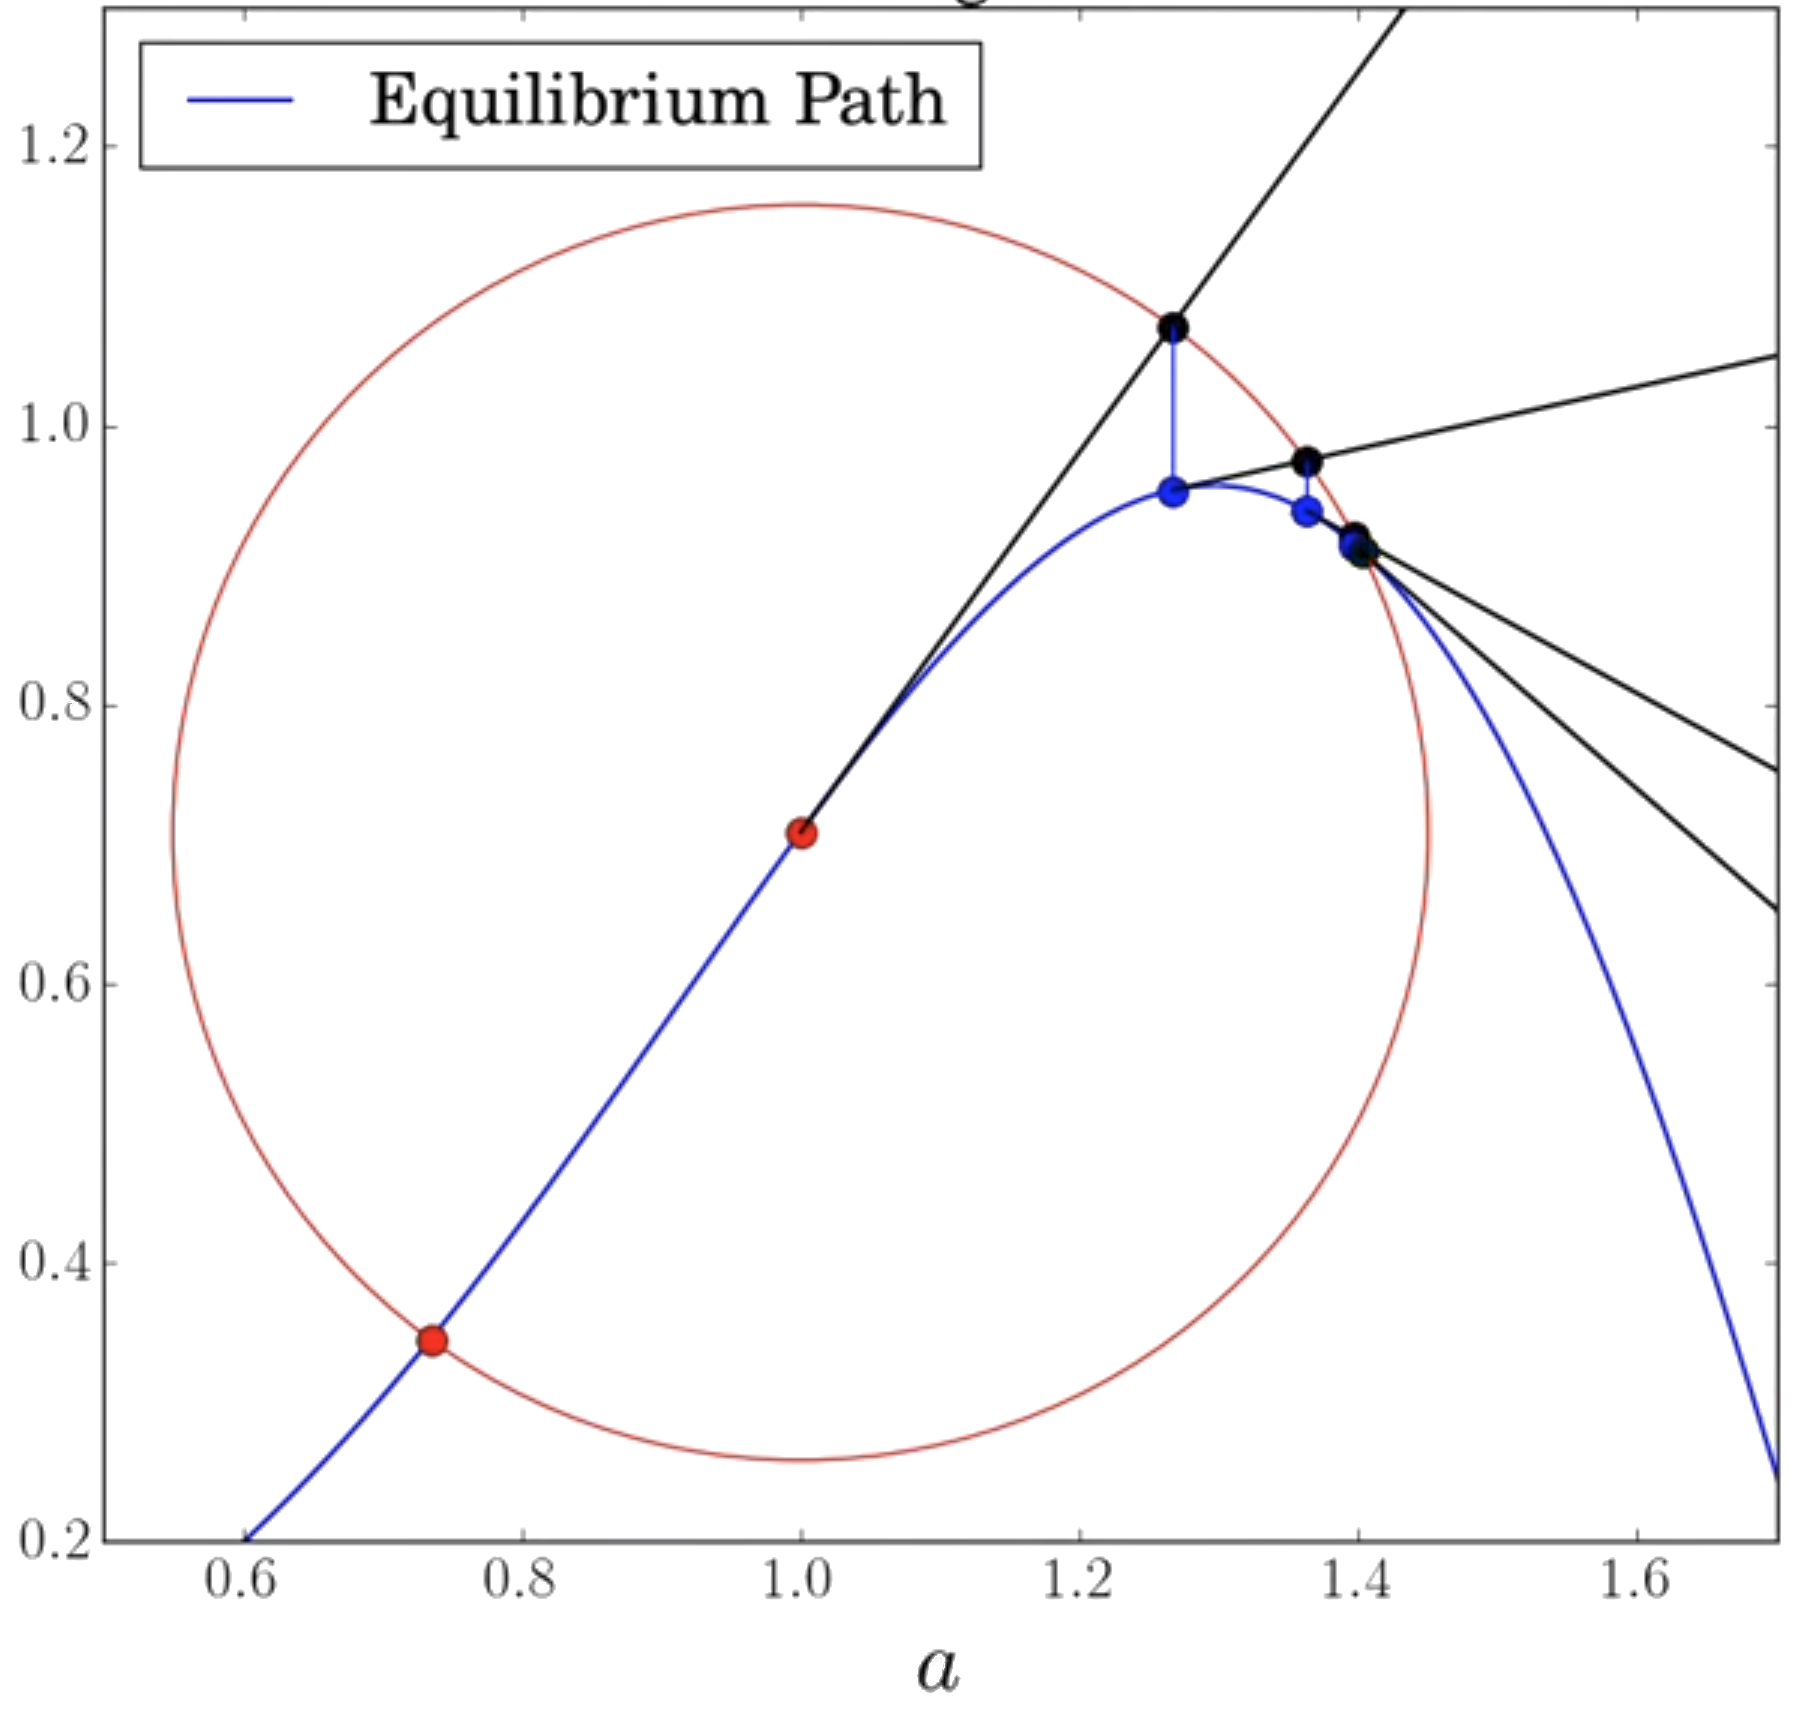
\includegraphics[width=0.65\textwidth]{figs/arc-length-visualized.png}
	\end{figure}
}
\mode<handout>{
	\vspace{6cm}
}
\end{frame}

\note{
	\begin{figure}[ht]
		\centering
		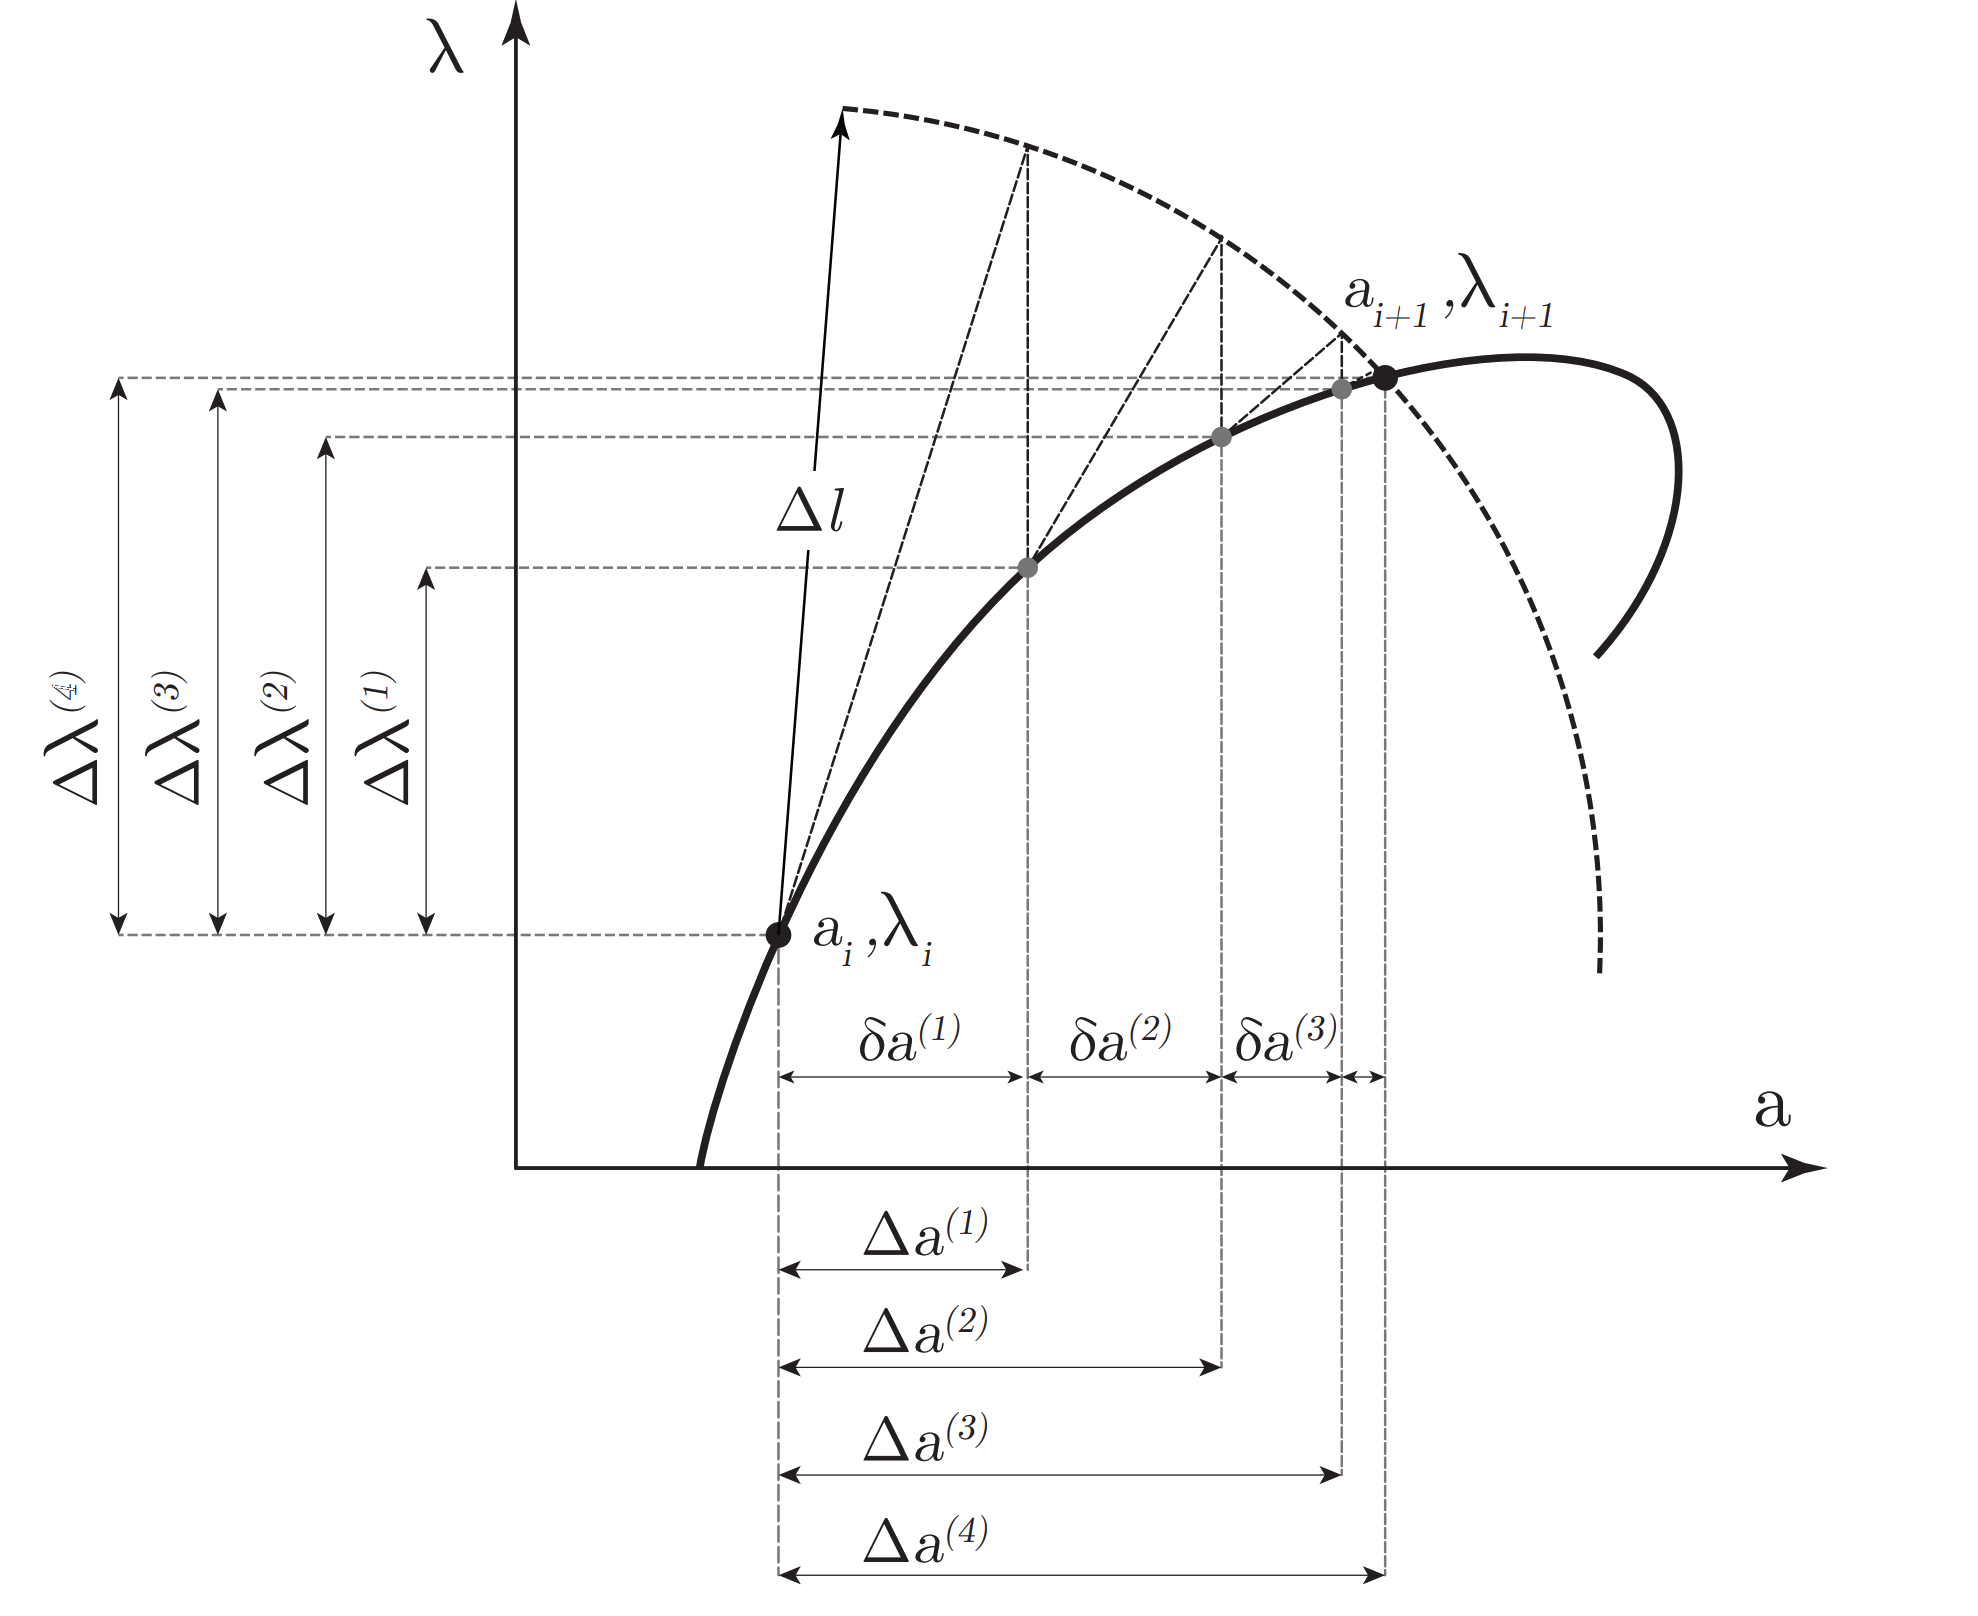
\includegraphics[width=0.8\textwidth]{figs/arc-length.png}
	\end{figure}
}


%------------------------------------------------
\begin{frame}
\frametitle{Arc length method: Drawbacks}
\mode<beamer>{
	\begin{figure}[ht]
		\centering
		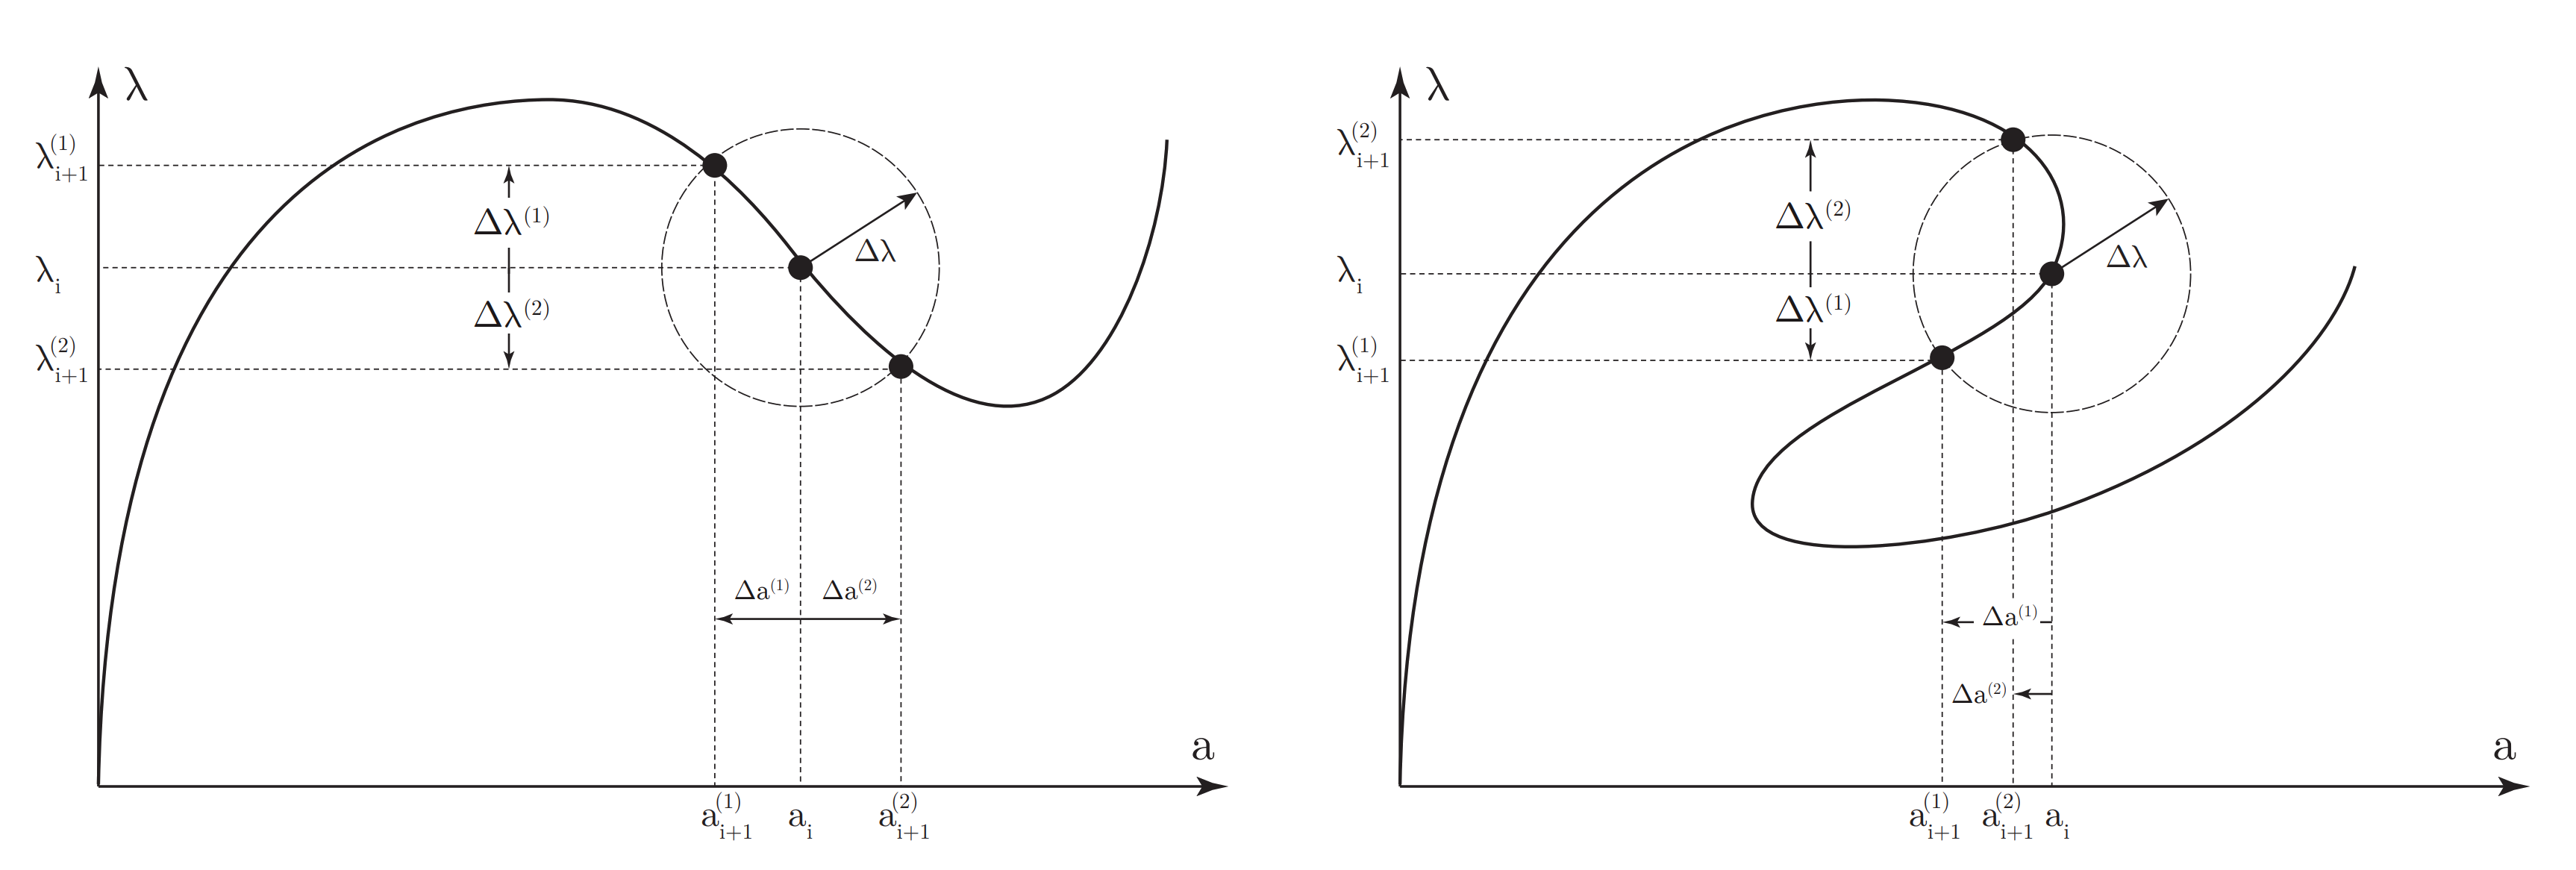
\includegraphics[width=\textwidth]{figs/arc-length-failure.png}
	\end{figure}
}
\mode<handout>{
	\vspace{6cm}
}
\end{frame}

\note {
Crisfield’s [1983] implementation of Arc-length however, leads to one of the method’s most important drawbacks. The quadratic equation would in general lead to two distinct solutions for $\delta \lambda$ which will in turn lead to two distinct solutions for $\delta u$. Thus, every iteration, the solver determined two sets of solutions, namely $(\delta u_1, \delta \lambda_1)$ and $(\delta u_1, \delta \lambda_1)$. This is no surprise since a circle (or a hyperellipse) would always intersect a curve in two points if its center is located on the curve.
}

\note {
The issue that arises then, is to develop a robust algorithm that would be able to accurately determine
the correct set of $(\delta u, \delta \lambda)$  to update the solution. In general, we would like to choose the set, so that the solution ‘evolves forwards’. This term ‘forward evolution’ is commonly used in the context of this method since choosing the wrong set would make the solution move back towards a previously converged point, and not in the desired (forward) direction. It is interesting to note, that an effective solution to this problem that works for all applications is yet to be found and as a result, many times programs like ABAQUS fail to converge to the correct solution or fail to ‘evolve forwards’.}

\section{Error estimates}
\subsection{A priori estimates}

%------------------------------------------------
\begin{frame}
\frametitle{A priori estimates}
\mode<beamer>{
	\begin{itemize}
		\item 	A priori error estimation is the analysis of the errors in a finite element simulation before
		actually performing an analysis. 
		\item It is an abstract concept since it cannot quantify the
		error in a computed simulation, but analysis can tell something about whether the finite
		element solution will converge to the exact solution as the mesh is refined, and how
		quickly it will converge if the element type is changed or the mesh is refined.

	\end{itemize}
}
\mode<handout>{
	\vspace{6cm}
}
\end{frame}

%------------------------------------------------
\begin{frame}
\frametitle{Functional norms}
Before considering the error, we need to decide how it should be measured. The question
is how to measure a function? The answer to this is to use function norms. A common
norm is known as the $L^2$ norm. For a function on a domain $\Omega$, the $L^2$ norm is defined
as:
\mode<beamer>{
	\begin{equation*}
	\left\lVert u \right\rVert_0 = \left(\int_\Omega u^2 d\Omega \right)^{1/2}
	\end{equation*}
}
\mode<handout>{
	\vspace{2cm}
}
This norm provides a measure of ‘how big’ a function is. A measure of the difference
between two functions $u$ and $v$ is provided by:
\mode<beamer>{
	\begin{equation*}
	\left\lVert u - v \right\rVert_0 = \left(\int_\Omega (u-v)^2 d\Omega \right)^{1/2}
	\end{equation*}
	
It is only possible that $\left\lVert u - v \right\rVert_0  = 0$ if $u = v$.
}
\mode<handout>{
	\vspace{2cm}
}
\end{frame}

%------------------------------------------------
\begin{frame}
\frametitle{Functional norms}
The $L^2$ norm measures the `magnitude' of a function, but does not reflect any details of
the derivatives. Other norms are the $H^1$ norm:
\mode<beamer>{
	\begin{equation*}
	\left\lVert u \right\rVert_0 = \left(\int_\Omega u^2 + \nabla u \cdot \nabla u d\Omega \right)^{1/2}
	\end{equation*}
}
\mode<handout>{
	\vspace{2cm}
}

We will use function norms to measure the difference between the exact solution and
the finite element solution. For example, we can define a particular measure of the error
$e$ as:
\mode<beamer>{
	\begin{equation*}
	\left\lVert u - u_h \right\rVert_0 = \left(\int_\Omega (u-u_h)^2 d\Omega \right)^{1/2}
	\end{equation*}
	where $u$ is the exact solution and $u_h$ is the finite element solution.
}
\mode<handout>{
	\vspace{2cm}
}
\end{frame}


%------------------------------------------------
\begin{frame}
\frametitle{How good is the FE solution?}
Inevitably, the finite element solution is not exact. But how do we know that it bears
any relation to the exact solution? If the mesh is refined, will the error reduce? We may
say intuitively yes, but this is not very satisfactory. This is where a priori analysis helps.
A priory error estimate:

\begin{equation*}
	\left\lVert u - u_h \right\rVert_s \le C h^\beta \left\lVert u  \right\rVert_{k+1}
\end{equation*}

\begin{itemize}
	\item $s$ is the norm of interest,
	\item $k$ is the polynomial order of the shape functions (complete polynomials), 
	\item $\beta = min (k + 1 - s, 2 (k + 1 - m))$,
	\item $m$ is the highest order derivative appearing in the weak form
	\item $C$ is an unknown constant that does not depend on $h$ or the exact solution $u$.
\end{itemize}
 What is of key interest is the exponent $\beta$.

\end{frame}


%------------------------------------------------
\begin{frame}
\frametitle{Error in the temperature/displacement field}
For a steady heat conduction or elasticity problem, for the error in the temperature/displacement field:

\mode<beamer>{
	\begin{itemize}
		\item $s = 0$
		\item $m = 1$
	\end{itemize}
}
\mode<handout>{
	\vspace{3cm}
}

Therefore, for $k \ge 1$,

\mode<beamer>{
	\begin{equation*}
		\left\lVert u - u_h \right\rVert_s \le C h^{k + 1} 	\left\lVert u  \right\rVert_{k+1}
	\end{equation*}
	
The solution converges with order $O(h^{k+1})$. Using quadratic shape functions, the error
converges with order $O(h^3)$. So, if the element size is halved, the error will be reduced
by a factor of eight.
}
\mode<handout>{
	\vspace{3cm}
}
\end{frame}


%------------------------------------------------
\begin{frame}
\frametitle{Error in the strain/flux field}
For a steady heat conduction or elasticity problem, for the error in the strain/flux field we have:
\mode<beamer>{
	\begin{itemize}
		\item $s = 1$
		\item $m = 1$
	\end{itemize}
}
\mode<handout>{
	\vspace{3cm}
}

Therefore, for $k \ge 1$,

\mode<beamer>{
	\begin{equation*}
	\left\lVert u - u_h \right\rVert_s \le C h^k \left\lVert u  \right\rVert_{k+1}
	\end{equation*}
	
	For a given element, the order of convergence in the first derivative is one order less than
	for the unknown field itself. Hence, the stresses in a finite element simulation are usually
	`\textit{less}' accurate than the displacements.
}
\mode<handout>{
	\vspace{3cm}
}
\end{frame}

\subsection{Posterior error estimation}
%------------------------------------------------
\begin{frame}
\frametitle{Posterior error estimation and adaptivity}
A \textit{posterior error} estimation involves quantification of the error after a simulation has
been preformed.\\

If we have an a posterior error estimator for a particular problem, a simulation can
been performed, the error estimated in various part of the domain and the mesh and
finite element type can be adjusted in order to reduce the error to a prescribed value.
This is known as \textit{adaptivity}. \\

The two obvious strategies are known as:
\mode<beamer>{
	\begin{itemize}
		\item \textit{h-adaptivity}: this involves modify the mesh.
		\item \textit{p-adaptivity}: this involves changing the finite element type.
	\end{itemize}
}
\mode<handout>{
	\vspace{3cm}
}
\end{frame}
\note{
A \textit{posterior error} estimation involves quantification of the error after a simulation has
been preformed. With an estimate of the error, a judgement can be made as to the 
reliability of the result. It is then also possible to adapt the finite element mesh to reduce the error. 
The goal of adaptivity is minimise the error for a given computational effort.
It is a rich area of activity in applied and computational mathematics.
}

%------------------------------------------------
\begin{frame}
\frametitle{Errors, compute-time, and memory}
An elasticity problem is solved on a square domain using a uniform structured mesh
of linear triangular elements with $n_1$ vertices in each direction ($n_1$ is very large).
\begin{figure}[ht]
	\centering
	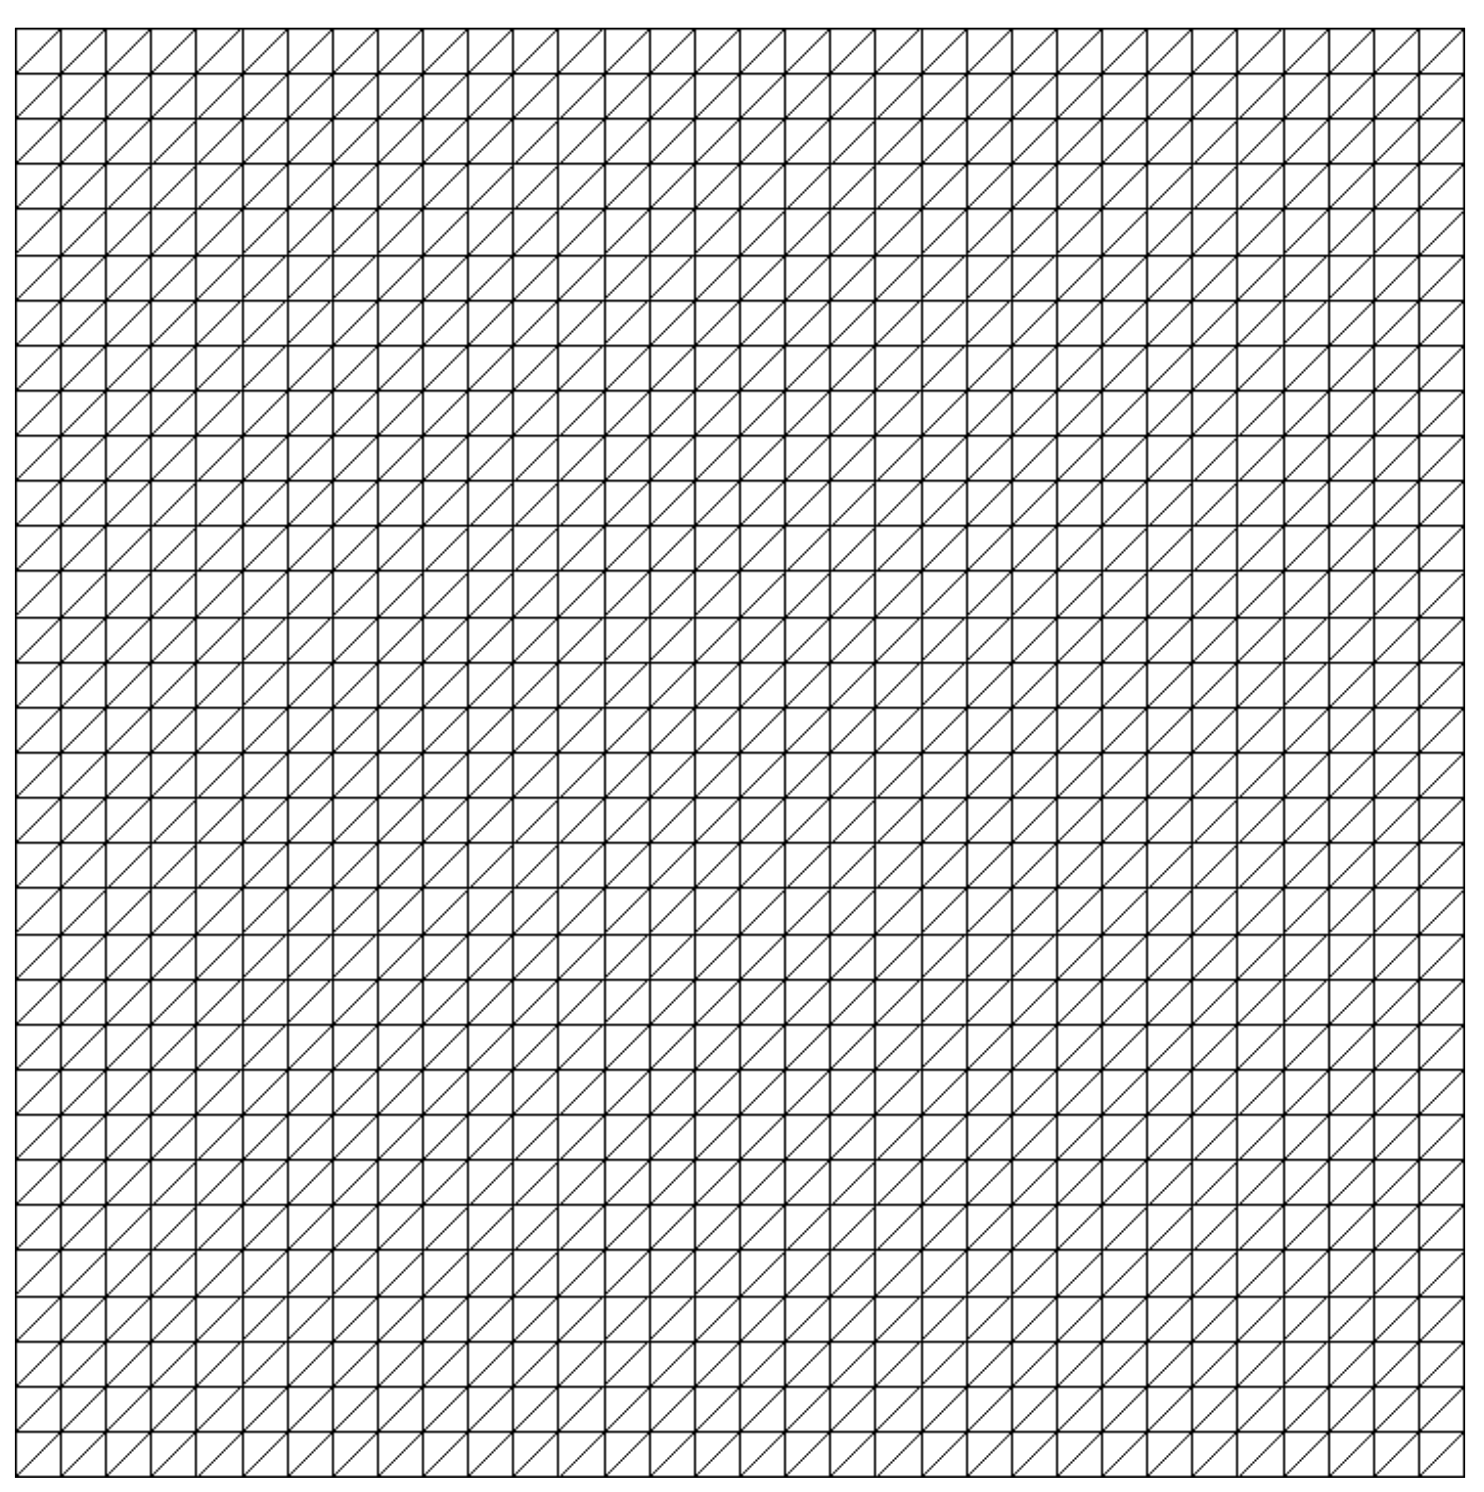
\includegraphics[width=0.5\textwidth]{figs/fe-mesh-errors.png}
\end{figure}
\end{frame}

%------------------------------------------------
\begin{frame}
\frametitle{Errors, compute-time, and memory}
\begin{enumerate}
	\item Based on a priori estimates, what reduction in the error could you expect?
	If the total number of elements is doubled and the element order is raised to quadratic,
	\item Provide an estimate of the increase in the required computational time if using
	LU decomposition.
	\item How much more computer memory is required to store the stiffness matrix?
	(Give the factor increase.)
\end{enumerate}
\end{frame}

\note{
\begin{figure}[ht]
	\centering
	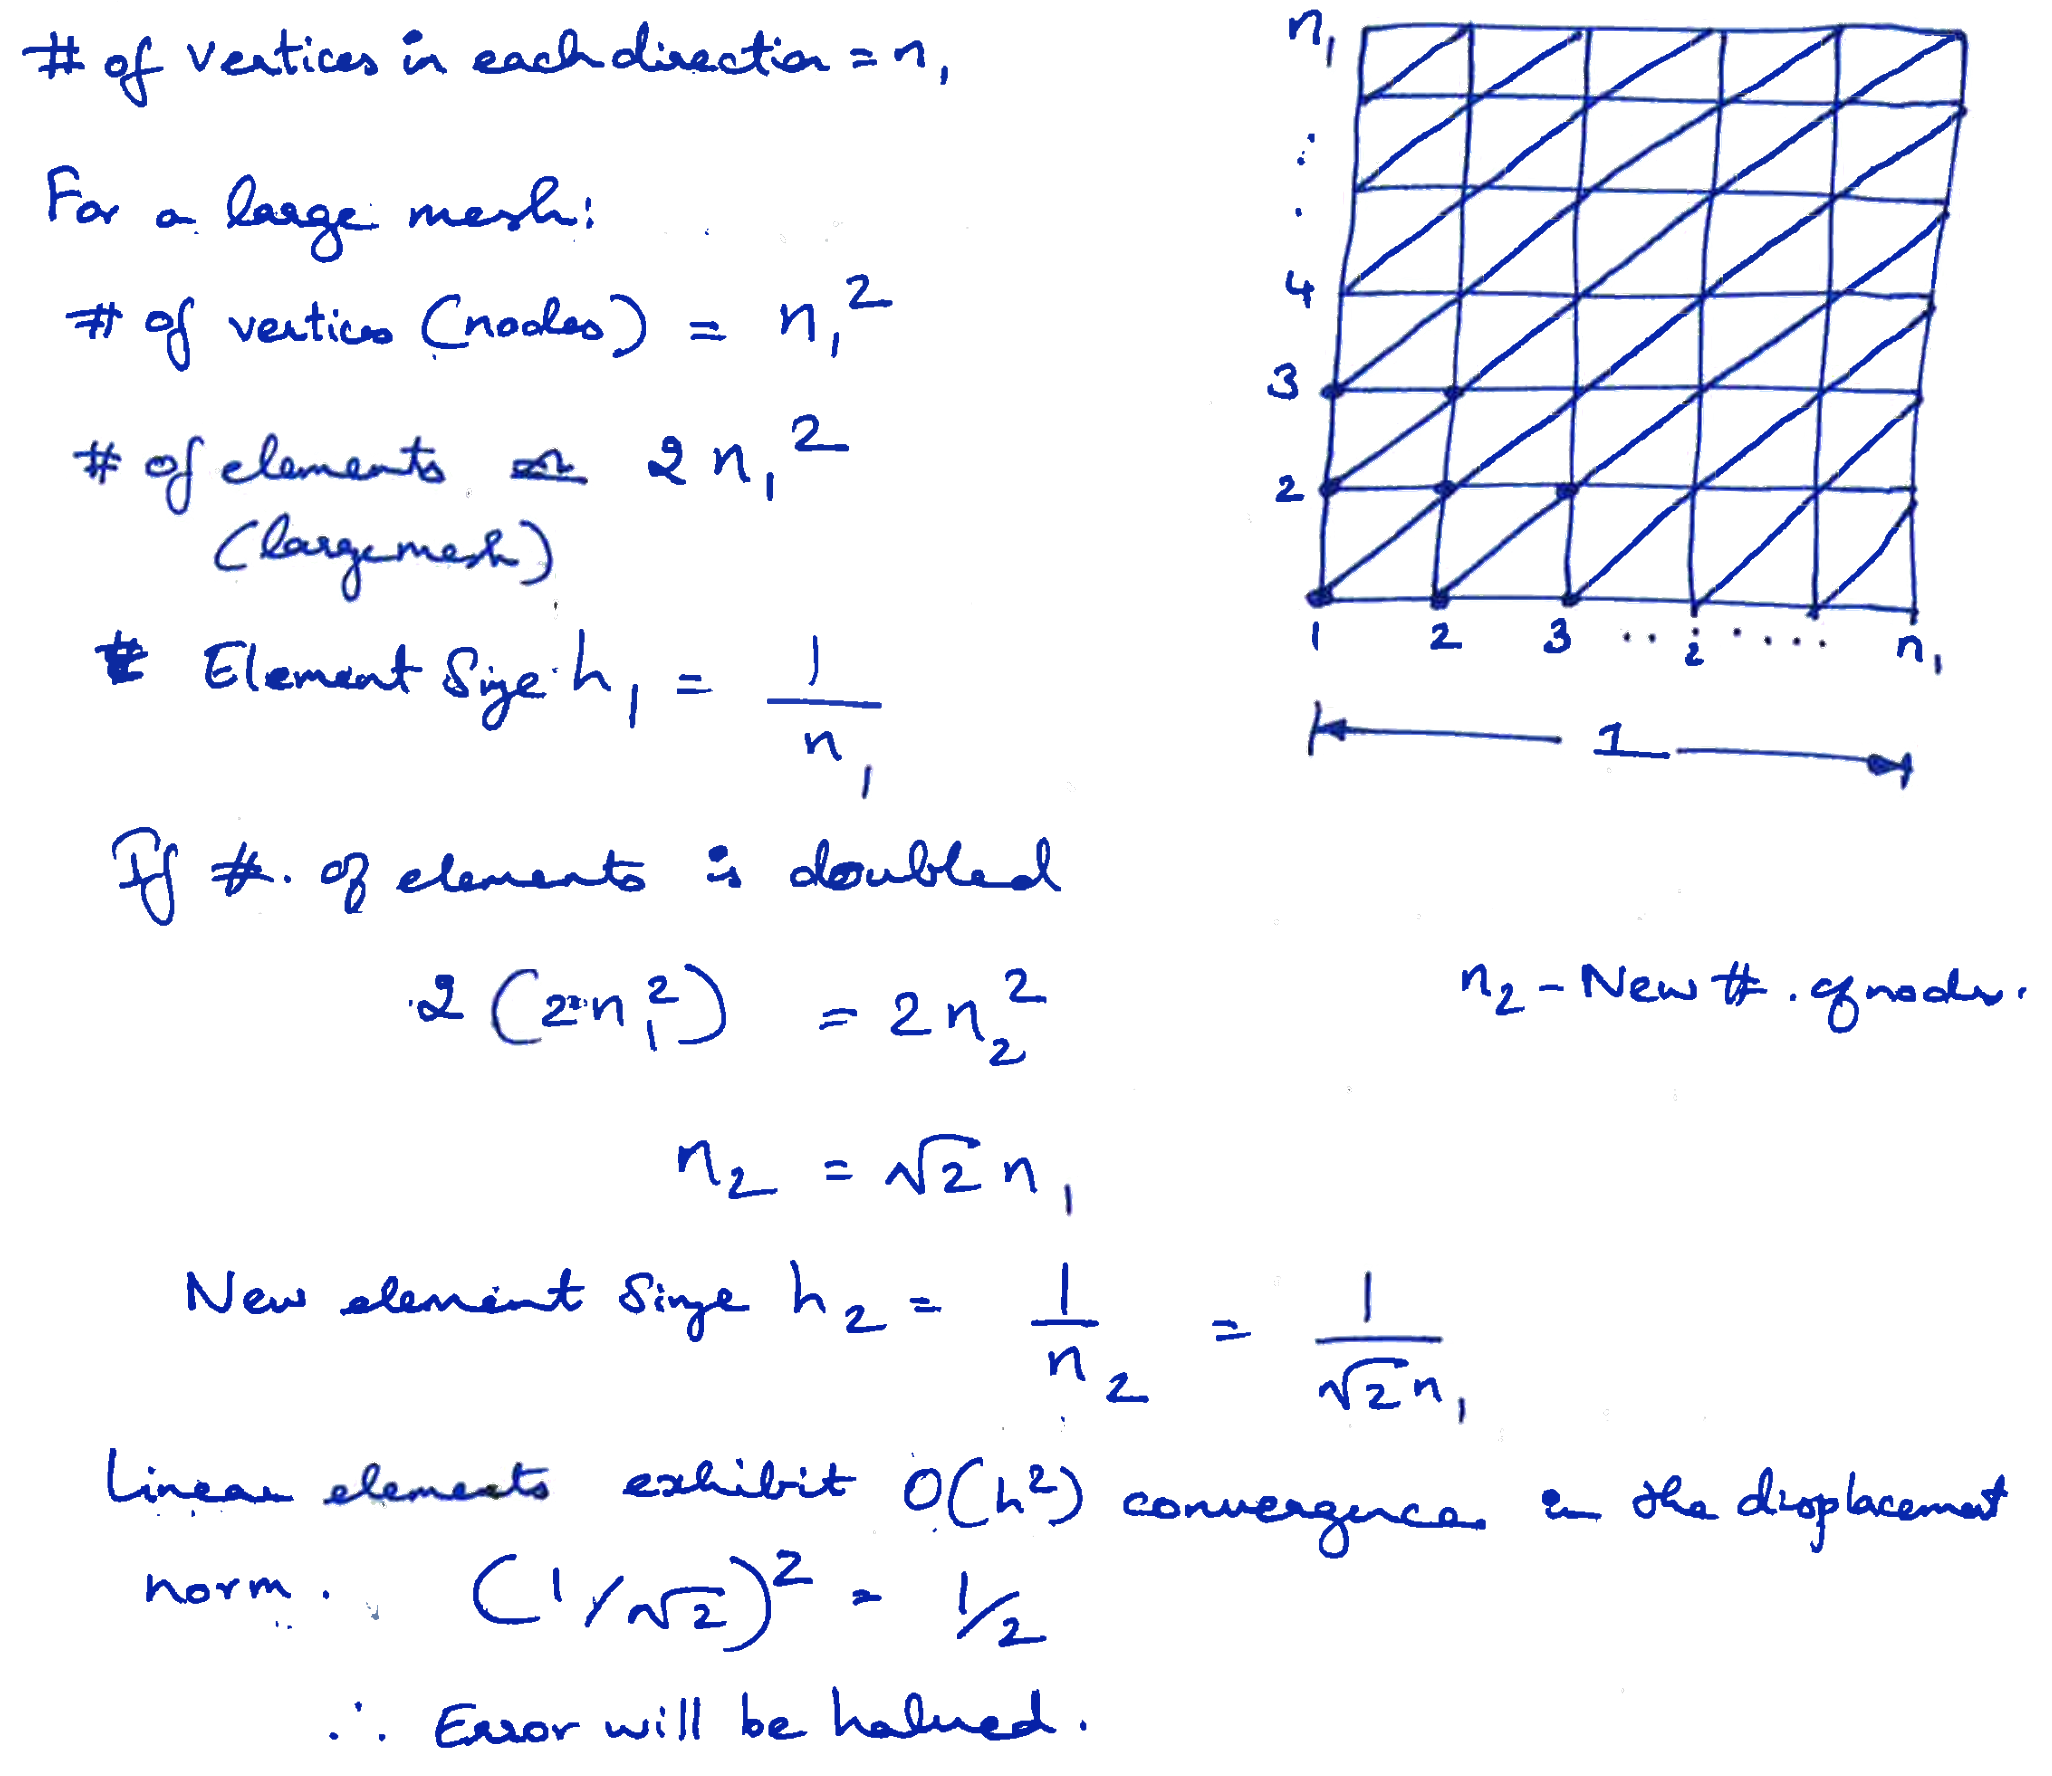
\includegraphics[width=0.72\textwidth]{figs/errors-mesh.png}
\end{figure}
}

\note{
	\begin{figure}[ht]
		\centering
		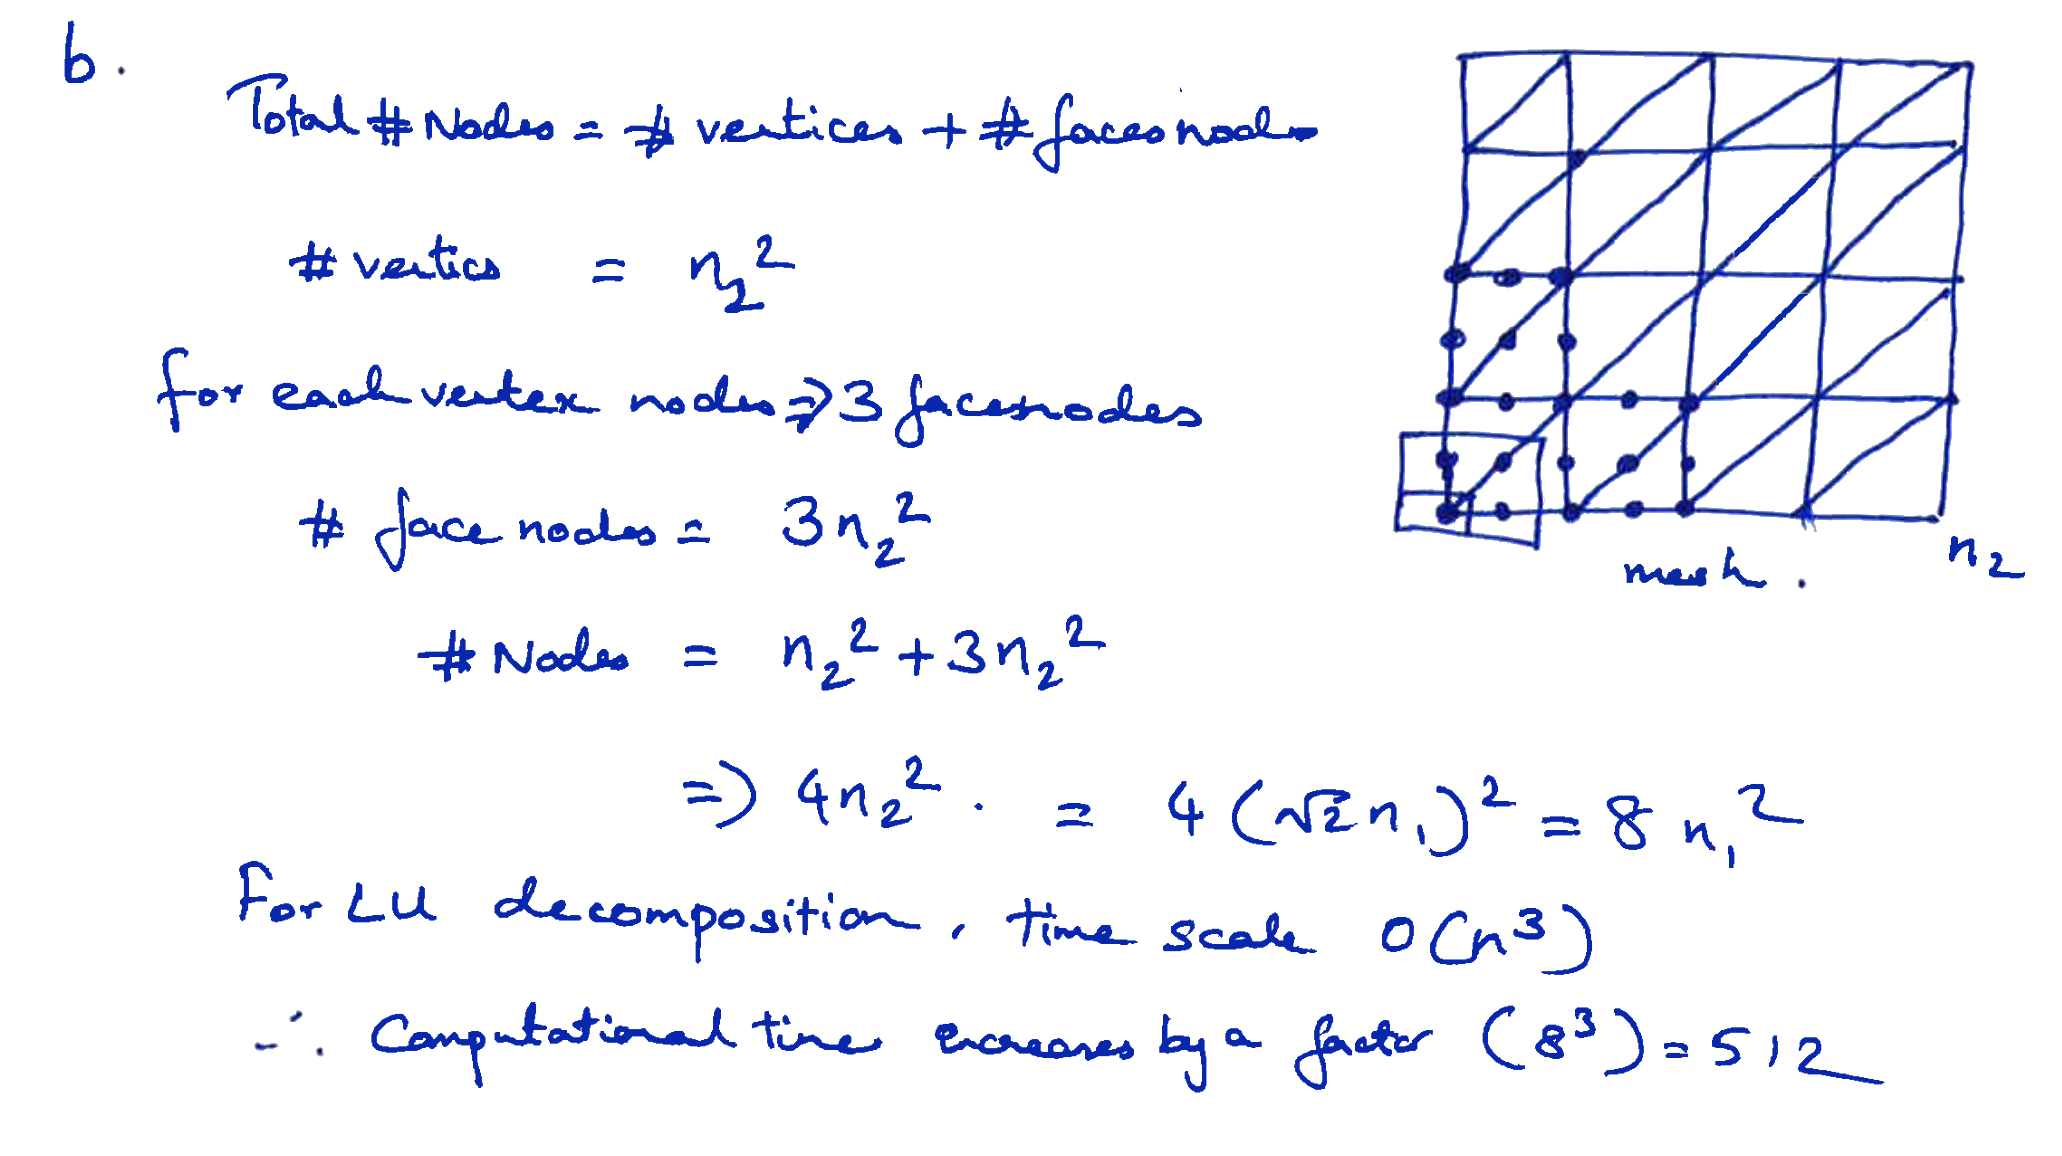
\includegraphics[width=0.72\textwidth]{figs/computational-time.png}
	\end{figure}
}


\note{
	\begin{figure}[ht]
		\centering
		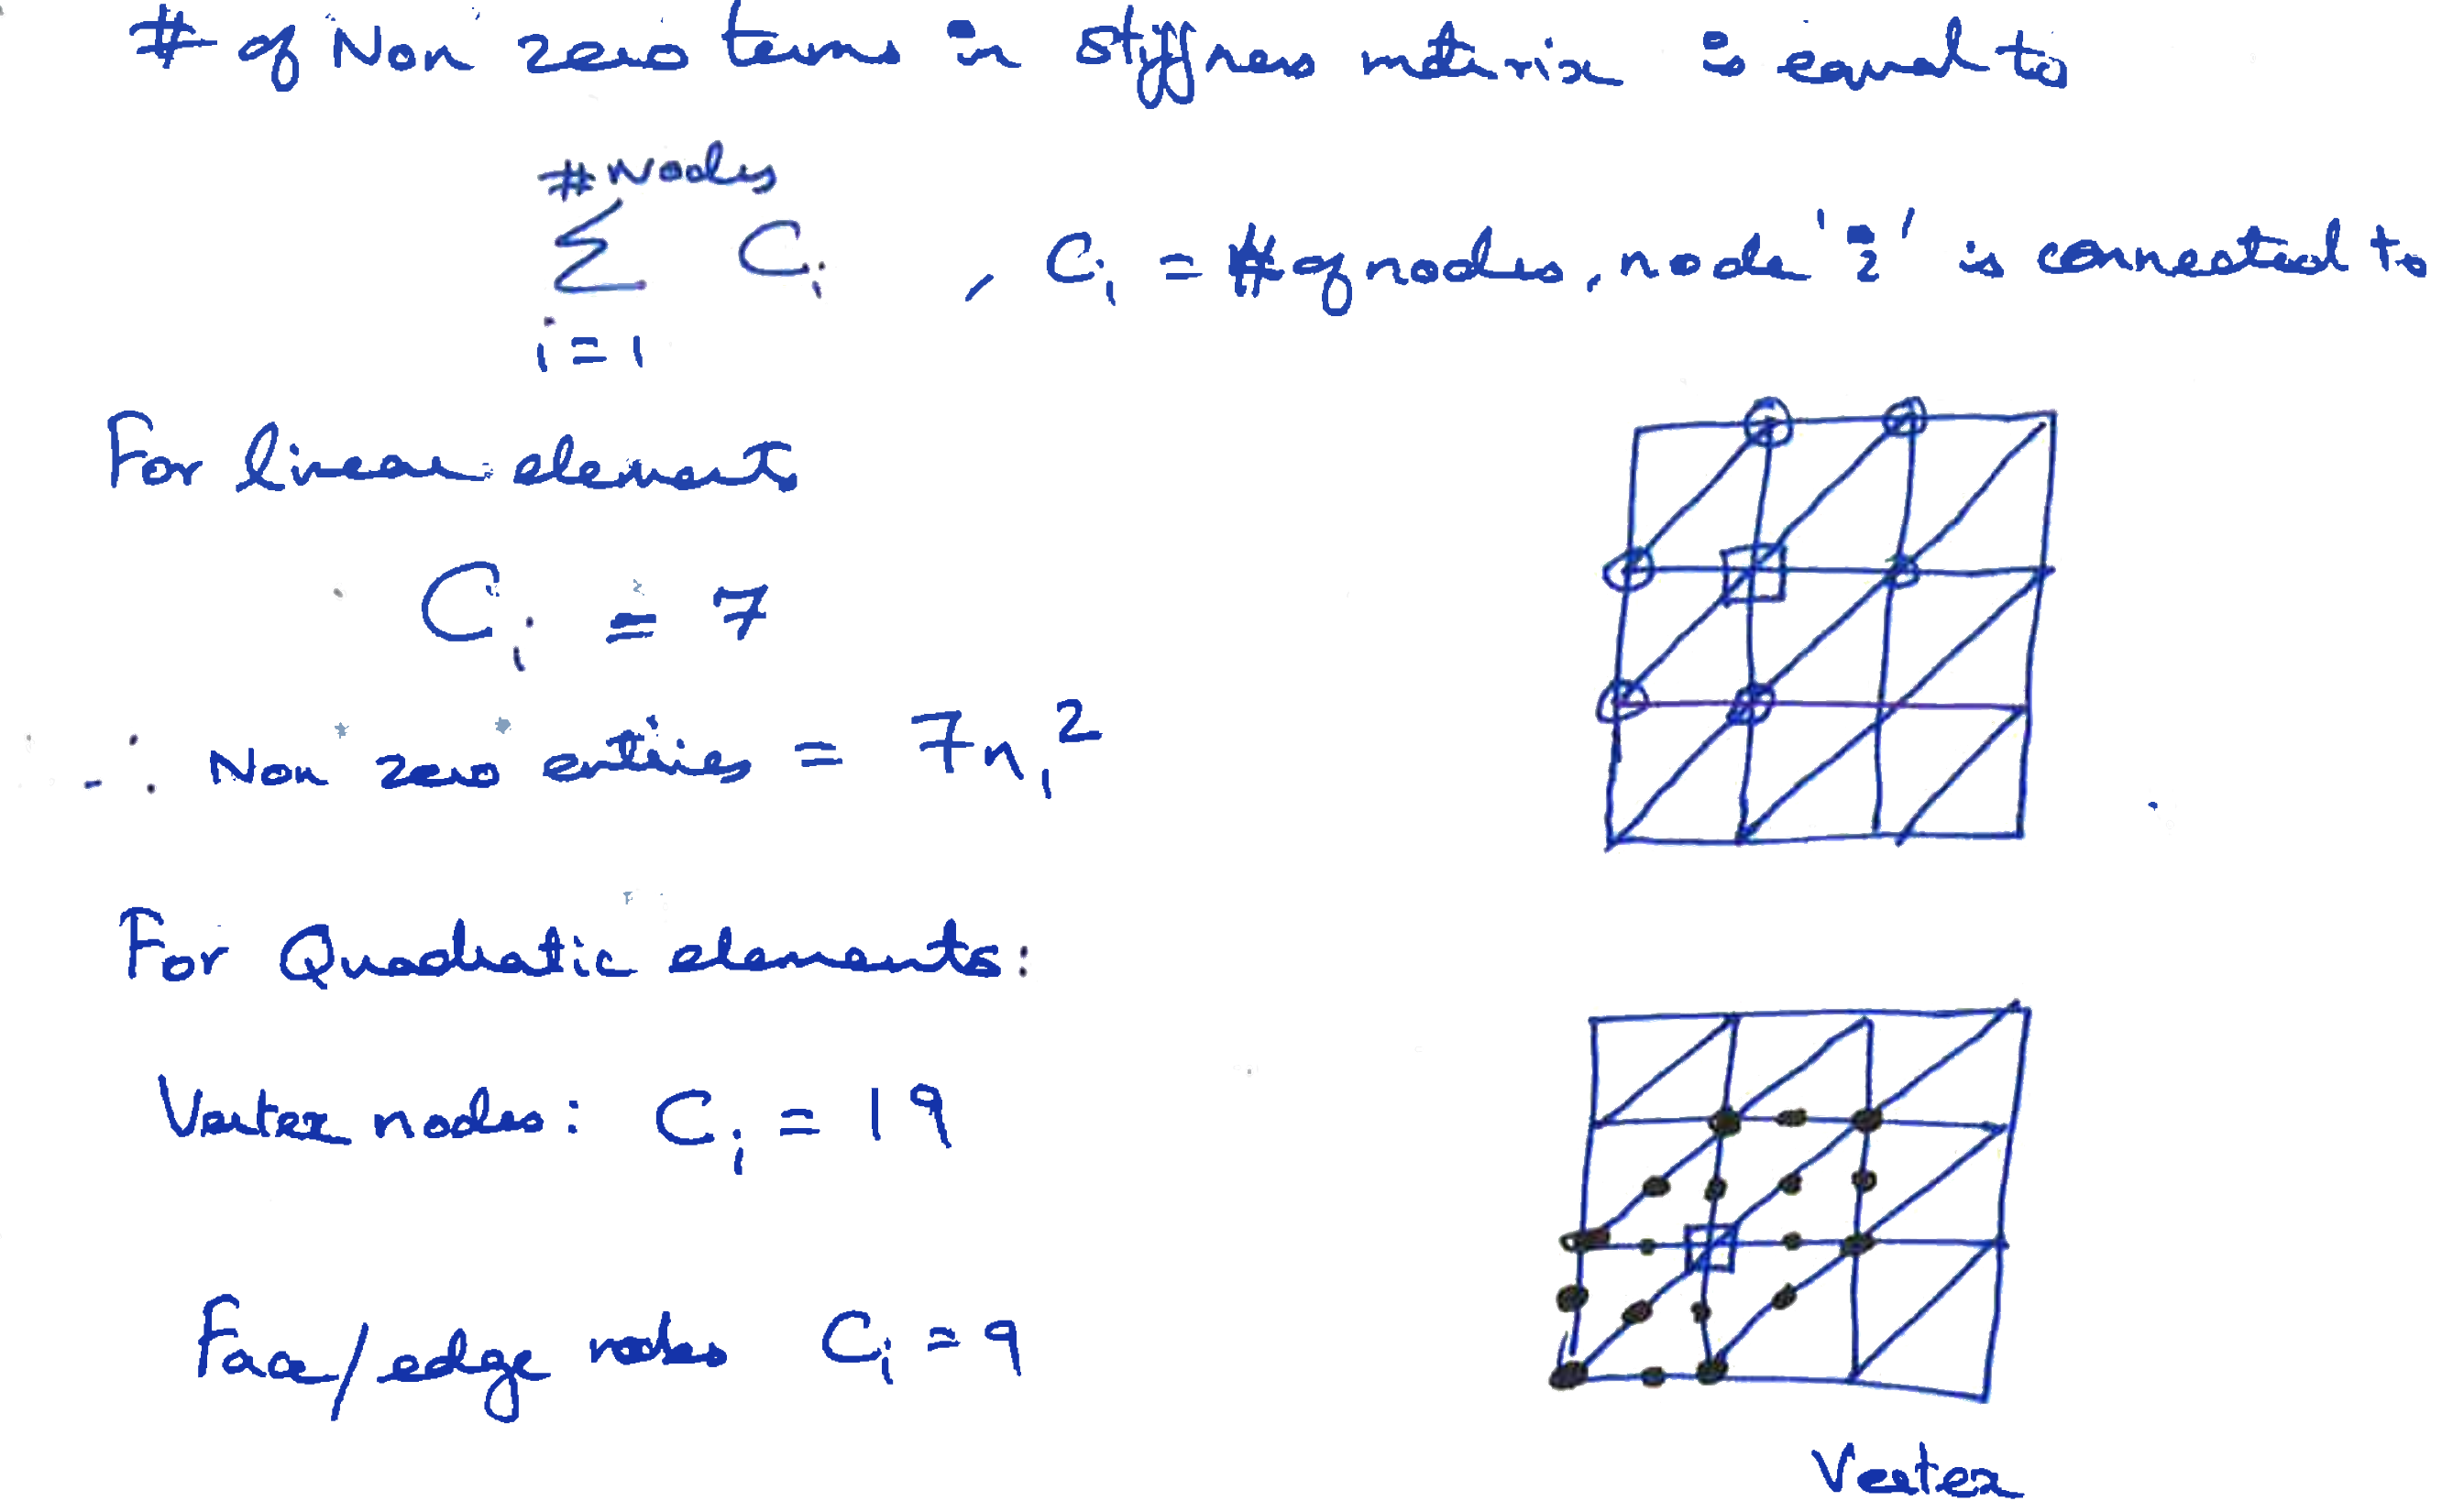
\includegraphics[width=0.72\textwidth]{figs/sparse-matrix-size.png}
	\end{figure}
}

\section{Time-dependent problems}
%------------------------------------------------
\begin{frame}
\frametitle{Time-dependent problems}

We wish to develop schemes to deal with semi-discrete finite element equations in a
step-by-step fashion. Starting at time $t = 0$, we want to solve a problem up to time
$t = t_{final}$. The time interval $(0, t_{final})$ will be `chopped' into increments $\Delta t$:
\begin{figure}[ht]
	\centering
	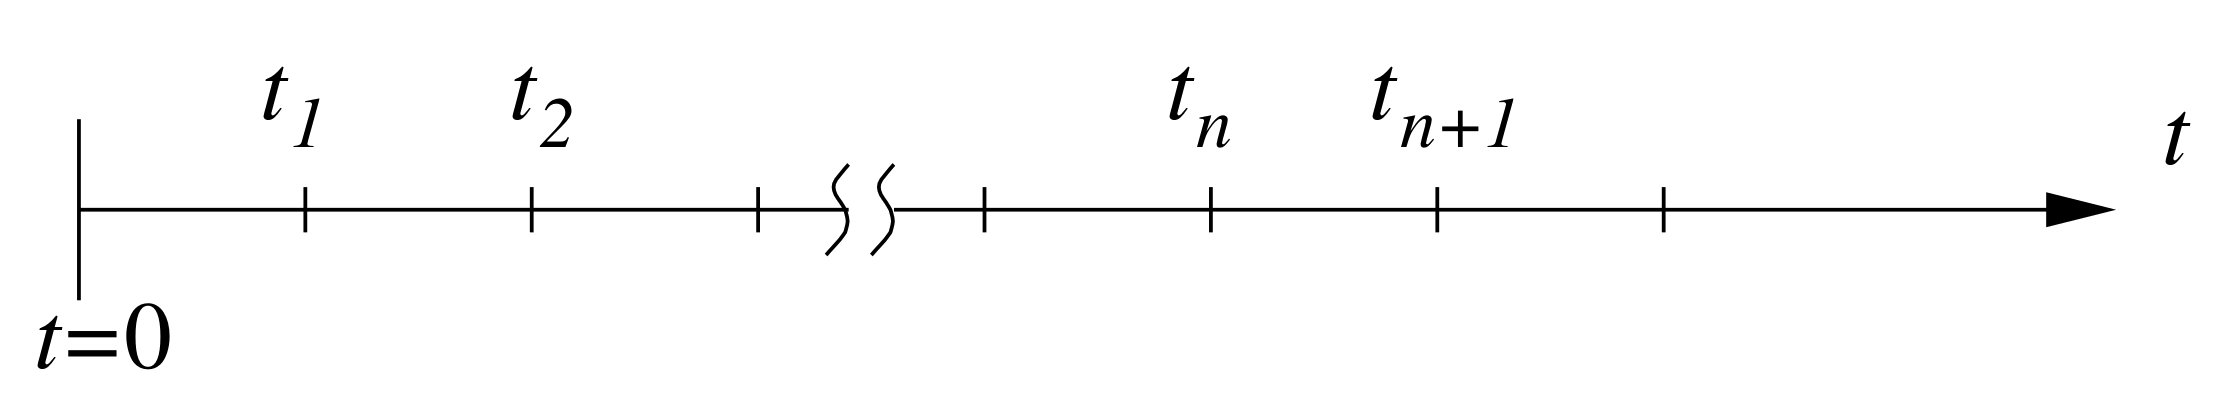
\includegraphics[width=0.65\textwidth]{figs/time-steps.png}
\end{figure}
\mode<beamer>{
	Time increment: $\Delta t = t_{n+1} - t_n$
}
\mode<handout>{
	\vspace{1cm}
}

What is needed is a strategy to advance the solution from $t_n$ to $t_{n+1}$. There are many
different techniques for this. We will consider some simple examples and the most commonly used methods.

\end{frame}

\subsection{Explicit schemes}
%------------------------------------------------
\begin{frame}
\frametitle{Forward Euler}
Given an equation of the form:
\begin{equation*}
	\dot{y}  = f(y, t)
\end{equation*}

for which we know everything at time $t_n(y_n\mathrm{ and } f(y_n, t_n))$,
we want to advance to time $t_{n+1}$ and find $y_{n+1}$. The simplest
approach is the forward Euler method. It involves:
\mode<beamer>{
	\begin{equation*}
		y_{n+1} = y_n + \Delta t f(y_n, t_n)
	\end{equation*}
	
Re-arranging,
	\begin{equation*}
		\frac{y_{n+1} - y_n }{\Delta t} = f(y_n, t_n)
	\end{equation*}
}
\mode<handout>{
	\vspace{4cm}
}
\end{frame}

%------------------------------------------------
\begin{frame}
\frametitle{Forward Euler}
\mode<beamer>{
	\begin{figure}[ht]
		\centering
		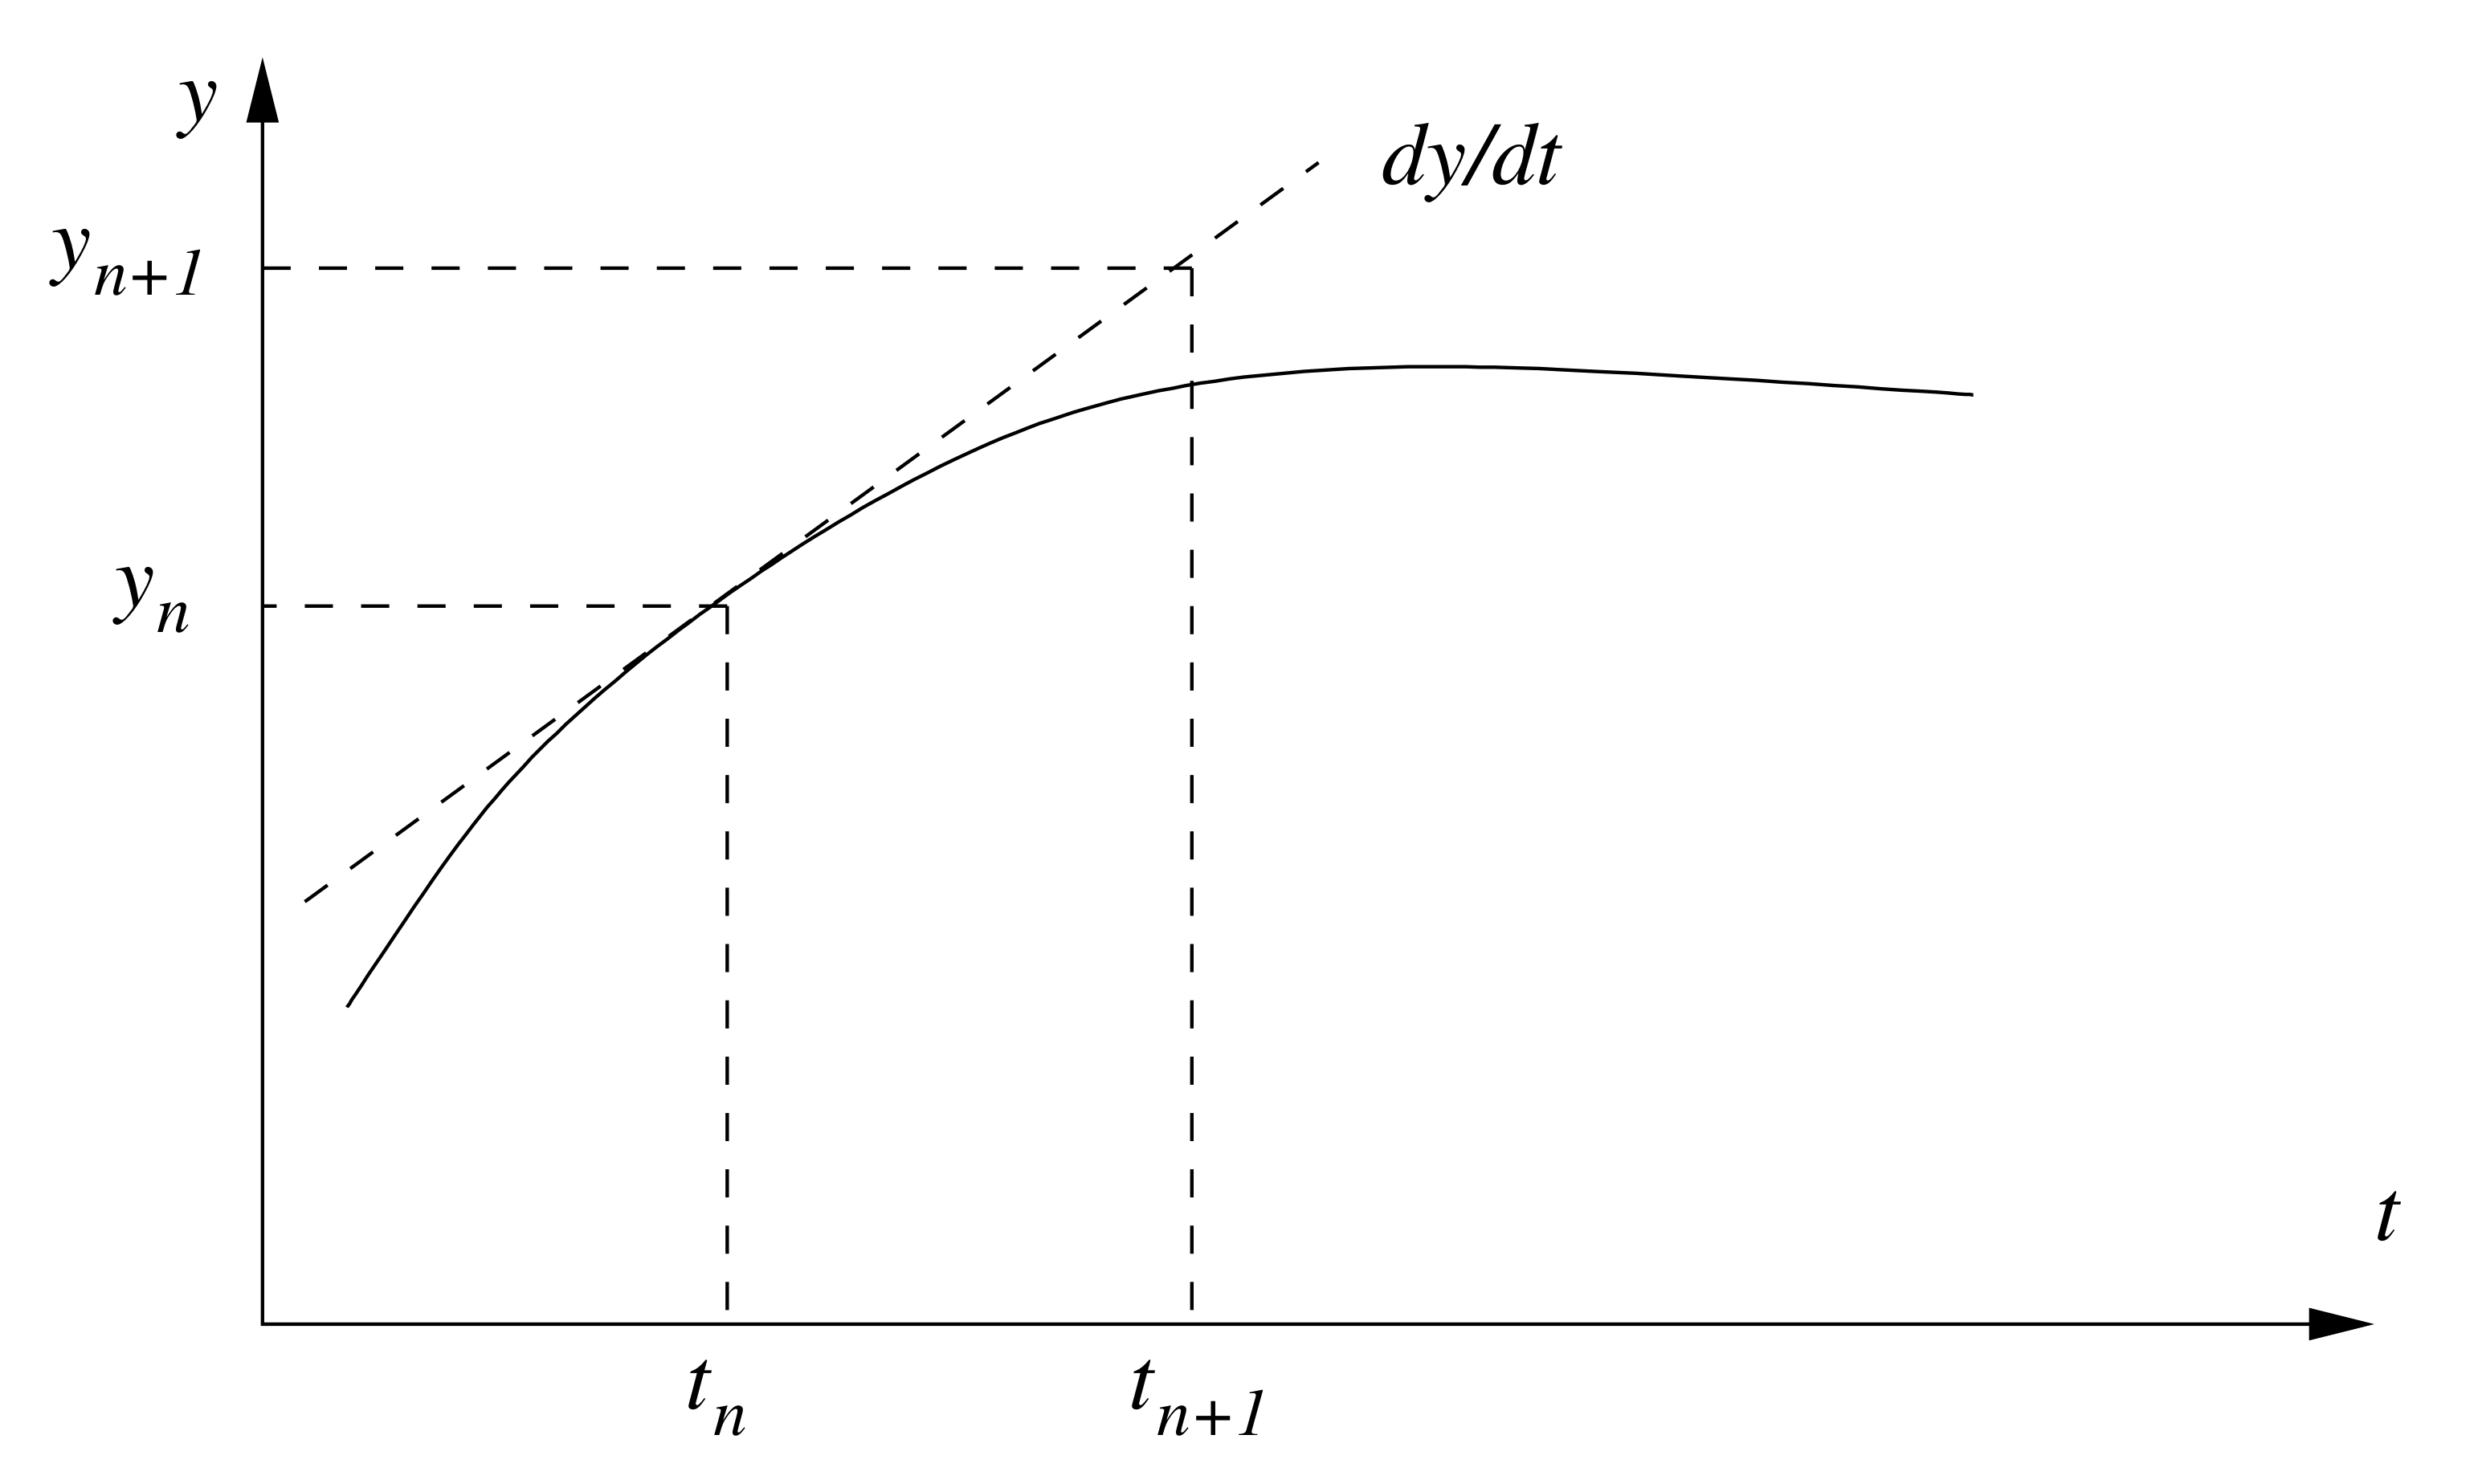
\includegraphics[width=\textwidth]{figs/forward-euler.png}
	\end{figure}
}
\mode<handout>{
	\vspace{6cm}
}
\end{frame}

%------------------------------------------------
\begin{frame}
\frametitle{Forward Euler}
We can apply the forward Euler scheme to the nodal degrees of freedom a by replacing
$y$ with $\mathbf{a}$ and $f$ with $\dot{\mathbf{a}}$,
\mode<beamer>{
	\begin{equation*}
	\frac{\mathbf{a}_{n+1} - \mathbf{a}_n }{\Delta t} = \dot{\mathbf{a}}_n
	\end{equation*}
}
\mode<handout>{
	\vspace{1cm}
}
We would like to eliminate the time derivative term $\dot{\mathbf{a}}$ from the semi-discrete heat equation, $\mathbf{M} \dot{\mathbf{a}} + \mathbf{Ka = b}$, so that we are left with only $\mathbf{a}$. In the forward Euler expression, we have $\dot{\mathbf{a}}_n$, therefore we consider the heat equation at time step $t_n$,
\mode<beamer>{
	\begin{equation*}
		\mathbf{M} \dot{\mathbf{a}}_n + \mathbf{K} \mathbf{a}_n = \mathbf{b}_n
	\end{equation*}

Inserting the forward Euler expression for $\dot{\mathbf{a}}$, we have

	\begin{equation*}
		\mathbf{M} \frac{\mathbf{a}_{n+1} - \mathbf{a}_n }{\Delta t} + \mathbf{K} \mathbf{a}_n = \mathbf{b}_n
	\end{equation*}
Taking all the known terms (those at $t_n$) to the right-hand side,

	\begin{equation*}
		\mathbf{M} \mathbf{a}_{n+1} = \mathbf{M} \mathbf{a}_n + \Delta t(\mathbf{b}_n - \mathbf{K} \mathbf{a}_n)
	\end{equation*}
}
\mode<handout>{
	\vspace{4cm}
}
\end{frame}

%------------------------------------------------
\begin{frame}
\frametitle{Forward Euler}
We have a system on linear equation that we can solve to find $\mathbf{a}_{n+1}$.
Now the benefit of a lumped mass matrix can be seen. If $\mathbf{M}$ is lumped, there is no
need to solve a system of equations and finding $\mathbf{a}_{n+1}$. is trivial.

System of equations for a lumped mass matrix:

\mode<beamer>{
	\begin{equation*}
		\begin{bmatrix}
			M_{11} & 0 & 0 \\
			0 & M_{22} & 0 \\
			0 & 0 & M_{33} \\
 		\end{bmatrix}
		\begin{bmatrix}
	 		a_{1, n+1} \\
	 		a_{2, n+1} \\
	 		a_{3, n+1} \\
 		\end{bmatrix} =
		\begin{bmatrix}
	 		\hat{b}_{1, n} \\
	 		\hat{b}_{2, n} \\
	 		\hat{b}_{3, n} \\
 		\end{bmatrix}
	\end{equation*}

Solution:
	\begin{equation*}
		a_{i, n+1} = \hat{b}_{i, n} / M_{ii}
	\end{equation*}
This is the key to the efficient simulation of some large scale time-dependent finite
element problems. We can start at $t =  0$ and advance in time. The process is simply repeated until the
desired final time is reached.
}
\mode<handout>{
	\vspace{4cm}
}
\end{frame}

\note{
	The forward Euler scheme is an example of an explicit scheme since $f$ depends only
	on data at $t_n$ (or possibly earlier steps). The forward Euler scheme is very simple, but
	unfortunately not very useful for the heat equation. Firstly, it is not particularly accurate
	(only $O(\Delta t)$), although this is not the biggest issue. The problem is stability. If 
	$\Delta t$ is too large, the solution a will grow rapidly and uncontrollably. The forward Euler method
	is notoriously unstable.
}

%------------------------------------------------
\begin{frame}
\frametitle{Forward Euler}
The time step at which a method becomes unstable is known at the \textit{critical time
step}. Conditionally stable methods are stable for: \mode<beamer>{$\Delta t \le \Delta t_{\mathrm{crit}}$}

\begin{itemize}
	\item The critical time step often scales with eigenvalues of the finite element system, which in turn depend on the element type and size. 
	\item As the element size is reduced, the critical time step reduces.
	\item The heat equation is a so-called stiff equation. This means that the restriction on the
	time step for explicit schemes is particularly severe. It scales according to \mode<beamer>{$\Delta t \propto h^2$}
\end{itemize}
where $h$ is a measure of the size of an element. This is a very strong restriction, and
means that explicit schemes are not usually practical for the heat equation.
\end{frame}


%------------------------------------------------
\begin{frame}
\frametitle{Second-order Central difference method}
\begin{align*}
	\dot{\mathbf{a}}_n & = \frac{\mathbf{a}_{n+1} - \mathbf{a}_{n-1} }{2\Delta t} \\
	\ddot{\mathbf{a}}_n & = \frac{\mathbf{a}_{n-1} -2 \mathbf{a}_n + \mathbf{a}_{n+1} }{\Delta t^2}
\end{align*}
	
This algorithm is explicit – it is possible	to express $\mathbf{a}_{n+1}$ in terms of quantities at $n$ and earlier times. This scheme is $O(\Delta t^2)$ 	accurate and it is conditionally stable. It is stable for:
	\begin{equation*}
	\Delta t \le \frac{2}{\omega_{h, max}}
	\end{equation*}
	
	where $\omega_{h, max}$ is the highest natural frequency. Therefore:
	
	\begin{equation*}
	\Delta t \le \frac{h}{c}
	\end{equation*}

where $c$ is the dilatation wave speed ($c = E/\rho$) and $h$ is the length of an element, which is the Courant, Friedrichs and Lewy (CFL) stability condition required for a wave to travel through an element.
\end{frame}

\subsection{Implicit method}
%------------------------------------------------
\begin{frame}
\frametitle{Backward Euler}
\mode<beamer>{
	\begin{equation*}
	y_{n+1} = y_n + \Delta t f(y_{n+1}, t_{n+1})
	\end{equation*}
}
\mode<handout>{
	\vspace{1cm}
}
Note now that $f$ is evaluated at $y_{n+1}$ and not at $y_n$. However, we do not know $y_{n+1}$; it
is what we want to find.
\mode<beamer>{
	\begin{align*}
	\mathbf{a}_{n+1} & =  \mathbf{a}_n + \Delta t \dot{\mathbf{a}}_{n+1} \\
	\frac{\mathbf{a}_{n+1} - \mathbf{a}_n }{\Delta t} & = \dot{\mathbf{a}}_n
	\end{align*}
}
\mode<handout>{
	\vspace{1.5cm}
}
Since the time derivative term is evaluated at $t_{n+1}$, we pose the semi-discrete heat
equation at $t_{n+1}$,
\mode<beamer>{
	\begin{equation*}
	\mathbf{M} \dot{\mathbf{a}}_{n+1} + \mathbf{K} \mathbf{a}_{n+1} = \mathbf{b}_{n+1}
	\end{equation*}
	
	Inserting the backward Euler expression for $\dot{\mathbf{a}}$, we have
	
	\begin{equation*}
	\mathbf{M} \frac{\mathbf{a}_{n+1} - \mathbf{a}_n }{\Delta t} + \mathbf{K} \mathbf{a}_{n+1} = \mathbf{b}_{n+1}
	\end{equation*}
}
\mode<handout>{
	\vspace{4cm}
}

\end{frame}


%------------------------------------------------
\begin{frame}
\frametitle{Backward Euler}
Collecting the unknown terms on the left-hand side and the known terms on the right-
hand side:
\mode<beamer>{
	\begin{equation*}
	\left(\mathbf{M} + \Delta t \mathbf{K}\right) \mathbf{a}_{n+1}  = \Delta t \mathbf{b}_{n+1} + \mathbf{M} \mathbf{a}_n
	\end{equation*}
}
\mode<handout>{
	\vspace{1.5cm}
}
\begin{itemize}
	\item Now, even if $\mathbf{M}$ is a diagonal matrix, we still need to solve a system of equations to find
	$\mathbf{a}_{n+1}$ because $\mathbf{K}$ is not diagonal. 
	
	\item A system must be solved because the backward Euler method is an \textit{implicit method}. 
	
	\item In stepping from $t_n$ to $t_{n+1}$, it relies on data at $t_{n+1}$ which is what characterises 
	implicit methods. 
	
	\item The consequence is that a system of equations must be solved.
\end{itemize}

\end{frame}

\note{
	The backward Euler method requires far more computational effort at each time step
	compared to the forward Euler method, yet it has the same order of accuracy $(O(\Delta t))$.
	However it is unconditionally stable. That is, there is no critical time step and the solution
	will remain bounded for any $\Delta t$. While each step is more expensive relative to an explicit
	method, it is possible that far fewer total steps will be required.
}


%------------------------------------------------
\begin{frame}
\frametitle{Summary of time-stepping schemes}

\mode<beamer>{
\begin{itemize}
	\item Explicit schemes are characterised by conditional stability.
	
	\item Explicit schemes can sometimes be very efficient as there is no need to solve systems
	of equations.
	
	\item Implicit schemes can be unconditionally stable (although not all implicit schemes
	are unconditionally stable).
	
	\item Implicit schemes require the solution of a system of equations, which can be expensive.
	
	\item Whether a scheme is explicit or implicit does not infer anything regarding accuracy.
\end{itemize}

}
\mode<handout>{
	\vspace{5cm}
}

\end{frame}

\end{document}